%%%% Document type  %%%%
\documentclass[preprint,12pt,fleqn]{article}
\usepackage{ragged2e}

% \usepackage{nopageno} % no page numbers
\usepackage{placeins} % \FloatBarrier
\usepackage{upgreek, bm}

\usepackage[most]{tcolorbox}
\newtcolorbox[auto counter,number within=chapter]{definition}[1][]{
  enhanced,
  breakable,
  fonttitle=\scshape,
  title={Definition \thetcbcounter},
  #1
}

%%%% Document structure %%%%
%\usepackage{geometry}
\usepackage[verbose=true,letterpaper]{geometry}
\geometry{
    textheight=9in,
    textwidth=6in,
    top=1in,
    headheight=12pt,
    headsep=25pt,
    footskip=30pt,
}

\usepackage{lineno} % used along with \linenumbers after begin document. 
\usepackage{setspace} 
% \setstretch{1.4}
\makeatletter % The following lines get rid of footer stating pre-preint to elsevier.
\def\ps@pprintTitle{%
\let\@oddhead\@empty
\let\@evenhead\@empty
\def\@oddfoot{}%
\let\@evenfoot\@oddfoot}
\makeatother
\graphicspath{ {../images/} }
\usepackage{pgf} % calculate cohort stats percentage

%%%% Bibliography   %%%%
\usepackage{natbib}
\setcitestyle{numbers,sort&compress}
\setcitestyle{sort&compress}
\usepackage{hypernat} 
    
%%%% Aesthetics     %%%%
\usepackage{microtype}
% \RequirePackage{times} % Font
\usepackage{ccaption}
\usepackage{siunitx}
\usepackage[T1]{fontenc}
\usepackage[utf8]{inputenc}
\usepackage{nameref}% this allows a reference be named, to print unnumbered references by their section name (used here for linking to Supplemental text in this case).

%%%% Paragraph Formatting %%%
\setlength{\parindent}{0pt}
\setlength{\parskip}{6pt plus 2pt minus 1pt}

%%%% Supplemental labels%%%%
%Define command to start a supplemental section
%set the supplemental letter used for figures (e.g. Figure E1)
\newcommand{\beginsupplement}{%
        \setcounter{table}{0}
        \renewcommand{\thetable}{S\arabic{table}}%
        \setcounter{figure}{0}
        \renewcommand{\thefigure}{S\arabic{figure}}%
         }

%%%% Building tables%%%%
\usepackage{booktabs} % required for tables
\usepackage{rotating,tabularx} 
\newcolumntype{Z}{ >{\centering\arraybackslash}X } % defining table content layout per box
\usepackage{ltablex} % allow page break between lines in tabularx
% \usepackage{caption} \captionsetup{font=normalsize} % to set the caption size as normal even when table is tiny.
\usepackage{multirow}
\usepackage{pdflscape}

%%%% Colors %%%%
\usepackage{xcolor} 
\definecolor{natureblue}{RGB}{5,110,210}
    \usepackage[colorlinks]{hyperref} 
\AtBeginDocument{%this allows colours to chage from the defined elsearticle template.
\hypersetup{
    	colorlinks=true,
        linkcolor={natureblue},
    	citecolor={natureblue},
        filecolor=blue!50!black,
        urlcolor=cyan,
    	}}

\definecolor{kispiblack}{HTML}{333333}
\definecolor{kispidarkblue}{HTML}{023047}
\definecolor{kispidarkgreen}{HTML}{006666}
\definecolor{kispired}{HTML}{C70000}
\definecolor{kispilink}{HTML}{007DB8}%219EBC
% \color{kispi_black} %default
\definecolor{kispiblue}{HTML}{701A57}
% City sunset: https://www.color-hex.com/color-palette/40131
\definecolor{colorSUNSET1}{HTML}{eeaf61}
\definecolor{colorSUNSET2}{HTML}{fb9062}
\definecolor{colorSUNSET3}{HTML}{ee5d6c}
\definecolor{colorSUNSET4}{HTML}{ce4993}
\definecolor{colorSUNSET5}{HTML}{6a0d83}
\definecolor{natureblue}{RGB}{5,110,210}    
\usepackage{dirtree}  % Load the dirtree package

% command to use these colors and formatting; xspace for correct spacing including with punctuation marks.
\usepackage{xspace}
\newcommand{\variablesdarkgreen}[1]{\textbf{\textcolor{kispidarkgreen}{#1}}\xspace}
 
\usepackage{tocloft}  % Customizing the Table of Contents
\setcounter{tocdepth}{2}

%%%% Include code %%%%
% \usepackage{verbatim}
\usepackage{listings}
\lstset{
    basicstyle=\ttfamily\small,
    breaklines=true,
    postbreak=\mbox{\textcolor{red}{$\hookrightarrow$}\space}, % 
    breakatwhitespace=false,
    % frame=single,
    showstringspaces=TRUE, % Don't show spaces in strings as special characters
    tabsize=2, 
    language=sh 
}

\usepackage{fontspec}

\usepackage[printonlyused,withpage,nohyperlinks]{acronym}
\usepackage{tikz}
\usetikzlibrary{calc}
\usepackage{amsmath, amssymb}

% author affil
\usepackage{authblk}
\renewcommand\Authfont{\normalsize}
\renewcommand\Affilfont{\small}
\setlength{\affilsep}{1em}

\begin{document}
\title{Quantifying prior probabilities for disease-causing variants reveals the top genetic contributors in inborn errors of immunity}

% in your preamble, before \author:
\newcommand{\QUANT}{1}
\newcommand{\GHI}{2}
\newcommand{\KISPIIMM}{3}
 \newcommand{\METAB}{4}
\newcommand{\LEEDS}{5}
\newcommand{\IPSNEO}{6}

\author[\QUANT]{Quant Group} 
\author[\GHI]{Simon Boutry}% \textsuperscript{†}}
\author[\GHI]{Ali Saadat}% \textsuperscript{†}} \textsuperscript{†}}
\author[\KISPIIMM]{Maarja Soomann}% \textsuperscript{†}} \textsuperscript{†}}
\author[\KISPIIMM]{Johannes Trück}
 \author[\METAB]{D. Sean Froese}
\author[\GHI]{Jacques Fellay}
\author[\LEEDS]{Sinisa Savic}% orcid.org/0000-0001-7910-0554
\author[\IPSNEO]{Luregn J. Schlapbach}
\author[\IPSNEO]{Dylan Lawless *%\thanks{Addresses for correspondence: \href{mailto:Dylan.Lawless@kispi.uzh.ch}{Dylan.Lawless@kispi.uzh.ch}}
}
% \textsuperscript{†}
\affil[\QUANT]{The quantitative omic epidemiology group.} 
\affil[\GHI]{Global Health Institute, School of Life Sciences, École Polytechnique Fédérale de Lausanne, Switzerland.}
\affil[\KISPIIMM]{Division of Immunology and the Children’s Research Center, University Children’s Hospital Zurich, University of Zurich, Zurich, Switzerland.}
 \affil[\METAB]{Division of Metabolism and Children’s Research Center, University Children’s Hospital Zürich, University of Zurich, Zurich, Switzerland.}
\affil[\LEEDS]{Leeds Institute of Rheumatic and Musculoskeletal Medicine, University of Leeds, Leeds, UK.}
\affil[\IPSNEO]{Department of Intensive Care and Neonatology, University Children's Hospital Zurich, University of Zurich, Zurich, Switzerland.}

\maketitle
\justify

%Abstract: 150 of 150. Main text:  3931 of 4000 (intro, result, discussion, conclusion). Display (4 figures / 2 tables) of 8 total. Extended display: 13 of 10. Note that this journal uses separate online methods.

\clearpage
 \linenumbers
\begin{abstract} 
We present a framework to quantify the prior probability of observing known disease-causing variants across all genes and inheritance modes. 
First, we computed genome-wide occurrence probabilities by integrating population allele frequencies, variant classifications, and Hardy-Weinberg expectations under autosomal dominant, recessive, and X-linked inheritance. 
Second, both pathogenic variants and missing causal candidates were tested to identify the most likely genetic disease determinant and provide a clear confidence range for the overall diagnosis. 
This provided a complete and interpretable summary of evidence for genetic diagnosis.
Third, we summarised variant probabilities for 557 genes responsible for inborn errors of immunity (IEI), now integrated into a public database. 
Fourth, we derived new data-driven IEI classifications using protein-protein interactions and curated clinical features, aligned to immunophenotypes. 
Finally, we validated the framework in national-scale cohorts, showing close concordance with observed case numbers. 
The resulting datasets supported causal variant interpretation and evidence-aware decision-making in clinical genetics.\footnote{
\noindent * Addresses for correspondence: \href{mailto:Dylan.Lawless@kispi.uzh.ch}{Dylan.Lawless@kispi.uzh.ch}.\\
% \noindent  \textsuperscript{† }These authors contributed equally and are listed alphabetically.\\
\textbf{Availability:} This data is integrated in public panels at 
% \url{https://switzerlandomics.ch/services/panelAppRexAi/} and 
\url{https://iei-genetics.github.io}.
The source code are accessible as part of the variant risk estimation project at \url{https://github.com/DylanLawless/var_risk_est} and IEI-genetics project at
\url{https://github.com/iei-genetics/iei-genetics.github.io}.
The data is available from the Zenodo repository: 
\url{https://doi.org/10.5281/zenodo.15111583}
(VarRiskEst PanelAppRex ID 398 gene variants.tsv).
VarRiskEst is available under the MIT licence.
% \url{https://github.com/TheQuantGroup/QauntGroup}.
}
\vfill
\end{abstract}


\noindent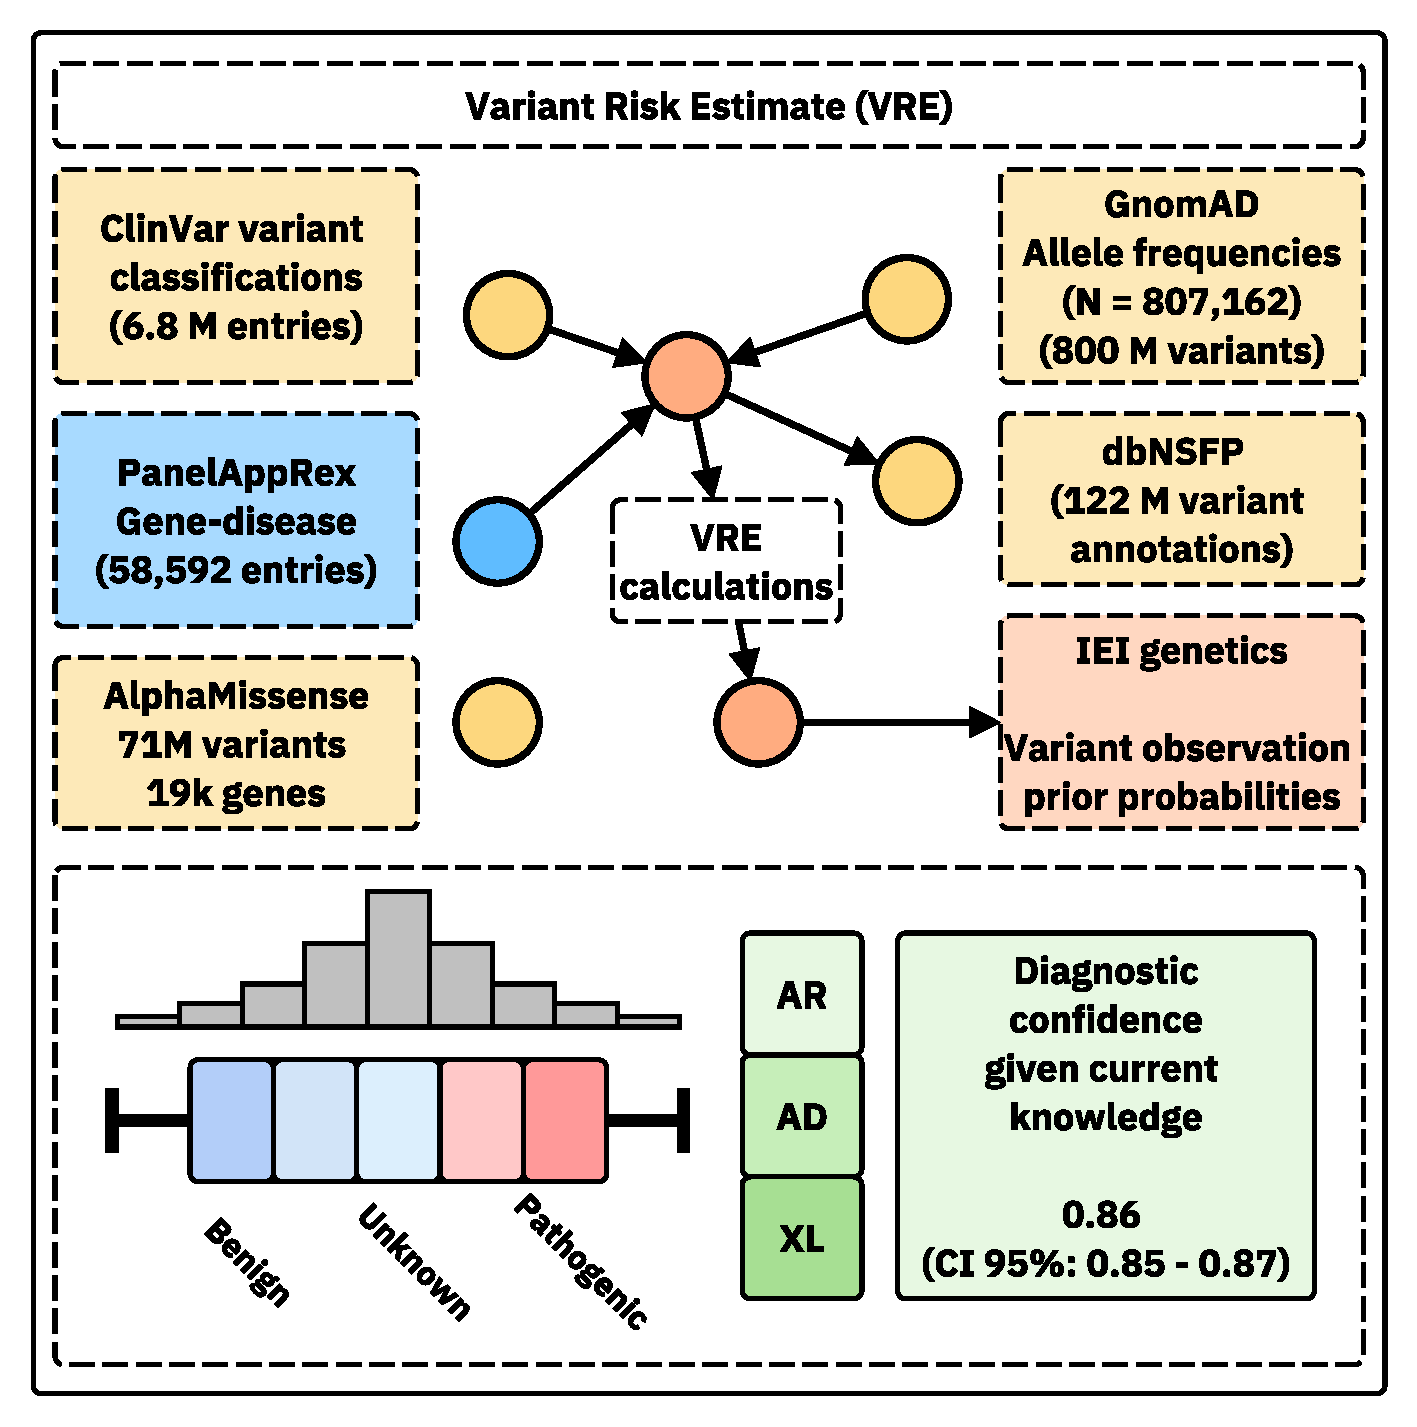
\includegraphics[width=0.99\textwidth]{../images/var_risk_est_ci.pdf}

Graphical abstract.

\clearpage


\section*{Acronyms}
\renewenvironment{description}%
  {\list{}{\labelwidth0pt\itemindent-\leftmargin
    \parsep-.5em\itemsep0pt\let\makelabel\descriptionlabel}}
  {\endlist}
\begin{acronym}
\acro{acmg}[ACMG]{American College of Medical Genetics and Genomics}%
\acro{acat}[ACAT]{Aggregated Cauchy Association Test}%
\acro{ad}[AD]{Autosomal Dominant}%
  \acro{af}[AF]{Allele Frequency}
 \acro{aid}[AID]{Autoinflammatory Disorders}
 \acro{anova}[ANOVA]{Analysis of Variance}
 \acro{ar}[AR]{Autosomal Recessive}
 \acro{bmf}[BMF]{Bone Marrow Failure}
 \acro{cd}[CD]{Complement Deficiencies}
 \acro{ci}[CI]{Confidence Interval}
 \acro{cri}[CrI]{Credible Interval}
 \acro{cid}[CID]{Immunodeficiencies affecting Cellular and Humoral Immunity}
 \acro{cid+}[CID+]{Combined Immunodeficiencies with Associated or Syndromic Features}
 \acro{cf}[CF]{Cystic Fibrosis}
 \acro{cftr}[\textit{CFTR}]{Cystic Fibrosis Transmembrane Conductance Regulator}
 \acro{cvid}[CVID]{Common Variable Immunodeficiency}
  \acro{dclre1c}[\textit{DCLRE1C}]{DNA Cross-Link Repair 1C}
 \acro{dbnsfp}[dbNSFP]{database for Non-Synonymous Functional Predictions}
 \acro{ge}[GE]{Genomics England} 
 \acro{gnomad}[gnomAD]{Genome Aggregation Database}
 \acro{grch38}[GRCh38]{Genome Reference Consortium Human Build 38}
\acro{gvcf}[gVCF]{genomic variant call format}
 \acro{hgvs}[HGVS]{Human Genome Variation Society}
 \acro{hpc}[HPC]{High-Performance Computing}
 \acro{hsd}[HSD]{Honestly Significant Difference}
 \acro{hwe}[HWE]{Hardy-Weinberg Equilibrium}
 \acro{iei}[IEI]{Inborn Errors of Immunity}
  \acro{ig}[Ig]{Immunoglobulin}
 \acro{il2rg}[\textit{IL2RG}]{Interleukin 2 Receptor Subunit Gamma}
 \acro{indel}[InDel]{Insertion/Deletion}
 \acro{iuis}[IUIS]{International Union of Immunological Societies}
 \acro{ld}[LD]{Linkage Disequilibrium}
 \acro{loeuf}[LOEUF]{Loss-Of-function Observed/Expected Upper bound Fraction}
 \acro{lof}[LOF]{Loss-of-Function}
 \acro{moi}[MOI]{Mode of Inheritance}
 \acro{nfkb1}[\textit{NFKB1}]{Nuclear Factor Kappa B Subunit 1}
 \acro{omim}[OMIM]{Online Mendelian Inheritance in Man}
 \acro{pad}[PAD]{Predominantly Antibody Deficiencies}
 \acro{pid}[PID]{Primary Immunodeficiency}
 \acro{pird}[PIRD]{Diseases of Immune Dysregulation}
 \acro{ppi}[PPI]{Protein-Protein Interaction}
 \acro{pli}[pLI]{Probability of being Loss-of-function Intolerant}
 \acro{qc}[QC]{Quality Control}
 \acro{rag1}[\textit{RAG1}]{Recombination activating gene 1}
 \acro{scid}[SCID]{Severe Combined Immunodeficiency}
 \acro{snv}[SNV]{Single Nucleotide Variant}
 \acro{skat}[SKAT]{Sequence Kernel Association Test}
 \acro{stringdb}[STRINGdb]{Search Tool for the Retrieval of Interacting Genes/Proteins}
 \acro{tp}[TP]{true positive}
\acro{fp}[FP]{false positive}
\acro{tn}[TN]{true negative}
\acro{fn}[FN]{false negative}
\acro{tnfaip3}[\textit{TNFAIP3}]{Tumor necrosis factor, alpha-induced protein 3}
 \acro{umap}[UMAP]{Uniform Manifold Approximation and Projection}
 \acro{uniprot}[UniProt]{Universal Protein Resource} 
 \acro{vcf}[VCF]{variant call format}
 \acro{vep}[VEP]{Variant Effect Predictor}
 \acro{vre}[VRE]{variant risk estimate}
 \acro{xl}[XL]{X-Linked}
\end{acronym}

\section{Introduction}

Accurately determining the probability that a patient harbours a disease-causing genetic variant remains a foundational challenge in clinical and statistical genetics. For over a century, the primary focus has been on identifying \ac{tp}s, pathogenic causal variants observed in affected individuals. 
Peer review and classification frameworks also work to suppress \ac{fp}s.
However, two critical components of the genetic landscape have received far less attention: \ac{fn}s, where pathogenic variants are missed due to technical or interpretive limitations, and \ac{tn}s, which represent the vast majority of benign or non-causal variants. 
\ac{tn}s are more commonly used in contexts such as cancer screening, where a negative result can provide reassurance that a panel of known actionable variants has been checked. Yet outside these specific uses, their broader statistical and clinical value is rarely leveraged.
From a statistical perspective, \ac{fn}s and \ac{tn}s are an untapped goldmine. 
They hold essential information about what is not observed, what should be expected under baseline assumptions, and how confident one can be in the absence of a pathogenic finding. 
Yet these dimensions are rarely quantified, leaving a bias in current variant interpretation frameworks towards known \ac{tp}s and lacking principled priors for genome-wide disease probability estimation.

Quantifying the risk that a patient inherits a disease-causing variant is a fundamental challenge in genomics. 
Classical statistical approaches grounded in \ac{hwe} \cite{MayoCentury2008, AbramovsHardyWeinberg2020} have long been used to calculate genetic probabilities for \ac{snv}s. 
However, applying these methods becomes more complex when accounting for different \ac{moi}, such as \ac{ar} versus \ac{ad} or \ac{xl} disorders. 
In \ac{ar} conditions, for example, the occurrence probability must incorporate both the homozygous state and compound heterozygosity, whereas for \ac{ad} and \ac{xl} disorders, a single pathogenic allele is sufficient to cause disease. 
Advances in genetic research have revealed that \ac{moi} can be even more complex \cite{zschocke_mendelian_2023}. 
Mechanisms such as dominant negative effects, haploinsufficiency, mosaicism, and digenic or epistatic interactions can further modulate disease risk and clinical presentation, underscoring the need for nuanced approaches in risk estimation.
\citet{karczewski2020mutational} made significant advances; however, the remaining challenge lies in applying the necessary statistical genomics data across all \ac{moi} for any gene-disease combination.
% which our current work aims to address.
Preliminary approaches have been reported for diseases such Wilson disease, mucopolysaccharidoses,  primary ciliary dyskinesia, and treatable metabolic diseasse, 
\cite{bick_estimating_2025, evans_estimating_2021}, 
as reviewed by \citet{hannah_using_2024}.

To our knowledge, all approaches to date have been limited to single \ac{moi}, specific to the given disease, or restricted to a small number of genes.
We argue that an  integrated approach is both necessary and highly powerful because the resulting probabilities can serve as informative priors in a Bayesian framework for variant and disease probability estimation; a perspective that is often overlooked in clinical and statistical genetics. 
Such a framework not only refines classical \ac{hwe}-based risk estimates but also has the potential to enrich clinicians’ understanding of what to expect in a patient and to enhance the analytical models employed by bioinformaticians.

The resulting dataset from these necessary calculations also holds value for AI and reinforcement learning applications, providing an enriched version of the data underpinning frameworks such as AlphaFold \cite{jumper_highly_2021} and AlphaMissense \cite{cheng_accurate_2023}.

This gap is not only due to conceptual limitations, but to the historical absence of large, harmonised reference datasets. 
Only recently have resources become available to support rigorous genome-wide probability estimation. These include high-resolution population allele frequencies (e.g. gnomAD v4 \cite{karczewski2020mutational}), 
curated variant classifications (e.g. ClinVar \cite{landrum_clinvar_2018}), 
functional annotations (e.g. UniProt \cite{the_uniprot_consortium_uniprot_2025}),
and pathogenicity prediction models (e.g. AlphaMissense \cite{cheng_accurate_2023}). 
% integrated gene-disease annotation platforms (e.g. PanelAppRex \cite{lawless_panelapprex_2025, martin_panelapp_2019}), 
We previously introduced PanelAppRex to aggregate gene panel data from multiple sources, including \ac{ge} PanelApp, ClinVar, and \ac{uniprot}, thereby enabling advanced natural searches for clinical and research applications \cite{lawless_panelapprex_2025, martin_panelapp_2019, landrum_clinvar_2018, the_uniprot_consortium_uniprot_2025}. 
This earlier work relied on expert-curated panels, such as those from the NHS National Genomic Test Directory and the 100,000 Genomes Project, converted into machine-readable formats for rapid variant discovery and interpretation. 
Together, these resources now make it possible to model the expected distribution of variant types, frequencies, and classifications across the genome.

By reframing variant interpretation as a problem of calibrated expectation rather than solely reactive confirmation, our framework empowers clinicians and researchers to anticipate both observed and unobserved pathogenic burdens. 
This scalable, genome-wide approach promises to streamline diagnostic workflows, reduce uncertainty in inconclusive cases, inform statistical models and genetic epidemiology studies, and accelerate the integration of genetic insights into patient care.

In this study, we focused on reporting the probability of disease observation through genome-wide assessments of gene-disease combinations. 
We then focused on known \ac{iei} genes, sometimes called the ``\ac{pid} or Monogenic Inflammatory Bowel Disease genes'' \cite{poli_human_2025, lawless_panelapprex_2025, martin_panelapp_2019},
to validate our approach and demonstrate its clinical relevance. 
This application to a well-established genotype-phenotype set, comprising over 500 gene-disease associations, underscores its utility.
The most recent update on the classification 
of \ac{iei} from the \ac{iuis}  expert committee was reported by \citet{poli_human_2025},
with an accompanying diagnostic guide \cite{bousfiha_2024_2025}.
Our central hypothesis was that by using highly curated annotation data including population \ac{af}s, disease phenotypes, \ac{moi} patterns, and variant classifications and by applying rigorous calculations based on \ac{hwe}, we could accurately estimate the expected probabilities of observing disease-associated variants.
Among other benefits, this knowledge can be used to derive genetic diagnosis confidence by incorporating these new priors.

%We previously introduced PanelAppRex to aggregate gene panel data from multiple sources, including \ac{ge} PanelApp, ClinVar, and \ac{uniprot}, thereby enabling advanced natural searches for clinical and research applications \cite{lawless_panelapprex_2025, martin_panelapp_2019, landrum_clinvar_2018, the_uniprot_consortium_uniprot_2025}. 
%It automatically retrieves expert-curated panels, such as those from the NHS National Genomic Test Directory and the 100,000 Genomes Project, and converts them into machine-readable formats for rapid variant discovery and interpretation. 
%We used PanelAppRex to label disease-associated variants.
%We also integrate key statistical genomic resources 
%including gnomAD which consists of over 900 million variants
%from over 800,000 individuals
%\cite{karczewski2020mutational},
%\ac{dbnsfp} which provides functional annotations for over 120 million potential variants 
%from 33 sources \cite{liu_dbnsfp_2020}, 
%and ClinVar which offers curated variant classifications such as ``Pathogenic'', ``Likely pathogenic'' and ``Benign'' mapped to \ac{hgvs} standards and expert reviews \cite{landrum_clinvar_2018}.

%To cite: \url{https://doi.org/10.1016/j.gimo.2024.101881} \url{https://doi.org/10.1016/j.gim.2024.101284} and some from 

\clearpage
\section{Methods}
\subsection{Dataset}

Data from \ac{gnomad} v4 comprised 807,162 individuals, including 730,947 exomes and 76,215 genomes \cite{karczewski2020mutational}. This dataset provided 786,500,648 \ac{snv}s and 122,583,462 \ac{indel}s, with variant type counts of 9,643,254 synonymous, 16,412,219 missense, 726,924 nonsense, 1,186,588 frameshift and 542,514 canonical splice site variants. ClinVar data were obtained from the variant summary dataset (as of: 16 March 2025) available from the NCBI FTP site, and included 6,845,091 entries, which were processed into 91,319 gene classification groups and a total of 38,983 gene classifications; for example, the gene \textit{A1BG} contained four variants classified as likely benign and 102 total entries \cite{landrum_clinvar_2018}. For our analysis phase we also used \ac{dbnsfp} which consisted of a number of annotations for 121,832,908 \ac{snv}s 
\cite{liu_dbnsfp_2020}. 
The PanelAppRex core model contained 58,592 entries consisting of 52 sets of annotations, including the gene name, disease-gene panel ID, diseases-related features, confidence measurements.
\cite{lawless_panelapprex_2025}
\ac{ppi} network data was provided by \ac{stringdb}, consisting of 19,566 proteins and 505,968 interactions \cite{szklarczyk2025string}.
The \ac{hgvs} nomenclature is used with \ac{vep}-based codes for variant IDs.
AlphaMissense includes pathogenicity prediction classifications for 71 million variants in 19 thousand human genes \cite{cheng_accurate_2023, jun_cheng_2023_8208688}. We used these scores to compared against the probability of observing the same given variants.
\textbf{Box \ref{box:definitions}} list the definitions from the \ac{iuis} \ac{iei} for the major disease categories used throughout this study \cite{poli_human_2025}.

The following genes were used for disease cohort validations and examples.
We used the two most commonly reported genes from the \ac{iei} panel \ac{nfkb1} 
\cite{tuijnenburgNFKB12018,
who1997primary,
cunningham1999common,
oksenhendler2008infections}
and \ac{cftr} 
\cite{naito2023uk, castellani2013cftr2, Grasemann2023cftr}
to demonstrate applications in \ac{ad} and \ac{ar} disease genes, respectively.
We used \ac{scid}-specific genes 
\ac{ar} \ac{dclre1c},
\ac{ar} \ac{rag1},
\ac{xl} \ac{il2rg} to demonstrate a \ac{iei} subset disease phenotype of 
\ac{scid}.
We also used \ac{ad} \ac{tnfaip3} for other examples comparable to \ac{nfkb1} since it is also causes \ac{ad} pro-inflammatory disease but has more known ClinVar classifications at higher \ac{af} then \ac{nfkb1}.

\begin{tcolorbox}[colback=black!01, colframe=black!70, title=Box \ref{box:definitions} Definitions for IEI Major Disease Categories, label=box:definitions]
\textbf{Major Category} \hspace{4em} \textbf{Description}\\[5pt]
1. CID  Immunodeficiencies affecting cellular and humoral immunity\\[2pt]
2. CID+  Combined immunodeficiencies with associated or syndromic features\\[2pt]
3. PAD - Predominantly Antibody Deficiencies\\[2pt]
4. PIRD - Diseases of Immune Dysregulation\\[2pt]
5. PD - Congenital defects of phagocyte number or function\\[2pt]
6. IID - Defects in intrinsic and innate immunity\\[2pt]
7. AID - Autoinflammatory Disorders\\[2pt]
8. CD - Complement Deficiencies\\[2pt]
9. BMF - Bone marrow failure
\end{tcolorbox}

\subsection{Variant classification occurrence probability}
To quantify the likelihood that an individual harbours a variant with a given disease classification, we compute the variant-level occurrence probability (\ac{vre}) for each variant.
As a starting point, we considered the classical \ac{hwe} for a biallelic locus:
\[
p^2 + 2pq + q^2 = 1,
\]
where \(p\) is the allele frequency, \(q = 1 - p\), \(p^2\) represents the homozygous dominant, \(2pq\) the heterozygous, and \(q^2\) the homozygous recessive genotype frequencies. For disease phenotypes, particularly under \ac{ar} \ac{moi}, the risk is traditionally linked to the homozygous state (\(p^2\)); however, to account for compound heterozygosity across multiple variants, %we extend this by incorporating the contribution from other pathogenic alleles.
we allocated the overall gene-level risk proportionally among variants.

Our computational pipeline estimated the probability of observing a disease-associated genotype for each variant and aggregated these probabilities by gene and ClinVar classification. This approach included all variant classifications, not limited solely to those deemed ``pathogenic'', and explicitly conditioned the classification on the given phenotype, recognising that a variant could only be considered pathogenic relative to a defined clinical context. The core calculations proceeded as follows:

\paragraph{1. Allele frequency and total variant frequency.} 
\label{sec:min_risk}
For each variant \(i\) in a gene, the allele frequency was denoted as \(p_i\). For each gene (any genomic region or set), we defined the total variant frequency (summing across all reported variants in that gene) as:

\[P_{\text{tot}} = \sum_{i \in \text{gene}} p_i.\]

Note that, because each calculation is confined to one gene, no additional scaling was required for our primary analyses (\(P_{\text{tot}}\)). However, if this same unscaled summation is applied across regions or variant sets of differing size or dosage sensitivity, it can bias burden estimates. In such cases, normalisation by region length or incorporation of gene- or region-specific dosage constraints is recommended.

If any of the possible \ac{snv}  had no observed allele (\(p_i = 0\)), we assigned a minimal risk:

\[p_i = \frac{1}{\max(AN) + 1}\]

where \(\max(AN)\) was the maximum allele number observed for that gene. This adjustment ensured that a nonzero risk was incorporated even in the absence of observed variants in the reference database.

%\paragraph{2. Occurrence probability based on \ac{moi}.}
%The probability that an individual was affected by a variant depended on the \ac{moi} relative to a specific phenotype. 
%Specifically, we calculated the occurrence probability \(p_{\text{disease},i}\) (\ac{vre}) for each variant as follows:
%\begin{itemize}
%    \item For \textbf{\ac{ad}} and \textbf{\ac{xl}} variants, a single copy was sufficient, so
%    \[
%    p_{\text{disease},i} = p_i.
%    \]
%    \item For \textbf{\ac{ar}} variants, disease is expected to manifest when two pathogenic alleles are present, either as homozygotes or as compound heterozygotes. 
%     We allocated the overall gene-level risk ($P_{\text{tot}}^2$) proportionally by variant allele frequency:
%% version 1 is wrong because it counted het variants twice: \[ p_{\text{disease},i} = p_i^2 + 2\,p_i\bigl(P_{\text{tot}} - p_i\bigr). \]
%    \[p_{\text{disease},i} = p_i \; P_{\text{tot}}.\] % version 2
%\end{itemize}

\paragraph{2. Occurrence probability based on \ac{moi}.}
The probability that an individual is affected by a variant depends on the \ac{moi}. For \textbf{\ac{ad}} and \textbf{\ac{xl}} variants, a single pathogenic allele suffices:

\[
p_{\text{disease},i} = p_i.
\]

For\textbf{ \ac{ar}} variants, disease manifests when two pathogenic alleles are present, either as homozygotes or as compound heterozygotes. We use:

\[p_{\text{disease},i} = p_i \; P_{\text{tot}}.\] % version 2

Under \ac{hwe}, the overall gene-level probability of an \ac{ar} genotype is

\[
P_{\text{AR}} \;=\; P_{\text{tot}}^2
\;=\;\sum_i p_i^2 \;+\; 2\sum_{i<j} p_i\,p_j,
\]

where \(P_{\text{tot}}=\sum_i p_i\). A naïve per-variant assignment

\[
p_i^2 + 2\,p_i\,(P_{\text{tot}} - p_i)
\]

would, when summed over all \(i\), double-count the compound heterozygous terms. 
To partition \(P_{\text{AR}}\) among variants without double counting, we allocate risk in proportion to each variant’s allele frequency:

\[
p_{\text{disease},i}
=\frac{p_i}{P_{\text{tot}}}\times P_{\text{tot}}^2
= p_i\,P_{\text{tot}}.
\]

This ensures

\[
\sum_i p_{\text{disease},i}
= \sum_i p_i\,P_{\text{tot}}
= P_{\text{tot}}^2,
\]

recovering the correct \ac{ar} risk while attributing each variant its fair share of homozygous and compound-heterozygous contributions.

More simply, for \ac{ad} or \ac{xl} conditions a single pathogenic allele suffices, so the classification risk (e.g. benign, pathogenic) equals its population frequency. For \ac{ar} conditions two pathogenic alleles are required - either two copies of the same variant or one copy each of two different variants, so we divide the overall recessive risk among variants according to each variant’s share of the total classification frequency in that gene.

\paragraph{3. Expected case numbers and case detection probability.}
Given a population with \(N\) births (e.g. as seen in our validation studies, \(N = 69\,433\,632\)), the expected number of cases attributable to variant \(i\) was calculated as:

\[
E_i = N \cdot p_{\text{disease},i}.
\]

The probability of detecting at least one affected individual for that variant was computed as:

\[
P(\geq 1)_i = 1 - \bigl(1 - p_{\text{disease},i}\bigr)^N.
\]

\paragraph{4. Aggregation by gene and ClinVar classification.}
For each gene and for each ClinVar classification (e.g. ``Pathogenic'', ``Likely pathogenic'', ``Uncertain significance'', etc.), we aggregated the results across all variants. The classification grouping can be substituted by any alternative score system. The total expected cases for a given group was:

\[
E_{\text{group}} = \sum_{i \in \text{group}} E_i,
\]

and the overall probability of observing at least one case within the group was calculated as:

\[
P_{\text{group}} = 1 - \prod_{i \in \text{group}} \left(1 - p_{\text{disease},i}\right).
\]

\paragraph{5. Data processing and implementation.}
We implemented the calculations within a \ac{hpc} pipeline and provided an example for a single dominant disease gene, \textit{TNFAIP3}, in the source code to enhance reproducibility. Variant data were imported in chunks from the annotation database for all chromosomes (1-22, X, Y, M). 

For each data chunk, the relevant fields were gene name, position, allele number, allele frequency, ClinVar classification, and HGVS annotations. 
Missing classifications (denoted by ``.'') were replaced with zeros and allele frequencies were converted to numeric values. % We then retained only the first transcript allele annotation for simplicity, as the analysis was based on genomic coordinates. 
Subsequently, the variant data were merged with gene panel data from PanelAppRex to obtain the disease-related \ac{moi} mode for each gene. 
For each gene, if no variant was observed for a given ClinVar classification (i.e. \(p_i = 0\)), a minimal risk was assigned as described above. 
Finally, we computed the occurrence probability, expected cases, and the probability of observing at least one case of disease using the equations presented.

The final results were aggregated by gene and ClinVar classification and used to generate summary statistics that reviewed the predicted disease observation probabilities.
We define the \emph{\ac{vre}} as the prior probability of observing a variant classified as the cause of disease 

\paragraph{6. Score-positive-total.}
For use as a simple summary statistic on the resulting user-interface, we defined the \emph{score-positive-total} as the total number of positively scored variant classifications within a given region (gene, locus, or variant set). 
Using the ClinVar classification assigned to a scale from$-5$ (benign) to $+5$ (pathogenic), we included only scores $> 0$, corresponding to some evidence of pathogenicity. 
The score-positive-total yields a non-normalised estimate of the prior probability that a phenotype is explained by known pathogenic variants.

\paragraph{7. Classification scoring system.}
\label{sec:classification_score}
Each ClinVar classification was assigned an integer score: pathogenic = +5, likely pathogenic = +4, pathogenic (low penetrance) = +3, likely pathogenic (low penetrance) = +2, conflicting pathogenicity = +2, likely risk allele/risk factor/association = +1, drug response/uncertain significance/no classification/affects/other/not provided/uncertain risk allele = 0, protective = –3, likely benign = –4, benign = –5. No further normalisation was applied. The resulting distribution (\textbf{Figure \ref{fig:p_gene_summary_hist_patch3} A-B}) is naturally comparable to a zero-centred average rank (\textbf{C-D}). This straightforward, modular approach can be readily replaced by any comparable evidence-based classification system. Variants with scores  $\leq 0$ were omitted, since benign classifications do not inform disease likelihood in the score-positive-total summary.

% --------------------------------------------------------------------------
% Methods, Results and Discussion: gene‑level pathogenic attribution
% --------------------------------------------------------------------------
\subsection{Integrating observed true positives and unobserved false negatives into a single, actionable conclusion}

In this section, we detail our approach to integrating sequencing data with prior classification evidence (e.g. pathogenic on ClinVar) to calculate the posterior probability of a complete successful genetic diagnosis.
Our method is designed to account for possible outcomes of 
\ac{tp},
% \ac{fp},
\ac{tn},
and \ac{fn},
by first ensuring that all nucleotides corresponding to known variant classifications (benign, pathogenic, etc.) have been accurately sequenced. 
This implies the use of \ac{gvcf}-style data which refer to \ac{vcf}s that contain a record for every position in the genome (or interval of interest) regardless of whether a variant was detected at that site or not.
Only after confirming that these positions match the reference alleles (or novel unaccounted variants are classified) do we calculate the probability that additional, alternative pathogenic variants (those not observed in the sequencing data) could be present. 
Our \ac{cri} for pathogenicity thus incorporates uncertainty from the entire process, including the tally of \ac{tp}, \ac{tn}, and \ac{fn} outcomes.
We ignore the contribution of \ac{fp}s  as a separate task to be tackled in the future.

We estimated, for every query (e.g. gene or disease-panel), the posterior probability that at least one constituent allele is both damaging and causal in the proband.  
The workflow comprises four consecutive stages.

\paragraph{(i) Data pre‑processing.}
We synthesized an example patient in a disease cohort of 200 cases.
We made several scenarios where a causal genetic diagnosis based on the available data is either simple, difficult, or impossible.
Our example focused on a proband two representative genes for \ac{ad} \ac{iei}: \ac{nfkb1} and  \ac{tnfaip3}.
All coding and canonical splice‑region variants for \ac{nfkb1} were extracted from the gVCF.  
We assumed a typical \ac{qc} scenario, where sites corresponding to previously reported pathogenic alleles were checked for read depth \mbox{$\ge\!10$} and genotype quality \mbox{$\ge\!20$}.  
Positions that failed this check were labelled \emph{missing}, thus separating true reference calls from non-sequenced or uninformative sequence.

\paragraph{(ii) Evidence mapping and occurrence probability.}
PanelAppRex variants were annotated with ClinVar clinical significance.  Each label was converted to an ordinal evidence score $S_i\in[-5,5]$ and rescaled to a pathogenic weight $W_i=\operatorname{rescale}(S_i;\,-5,5\rightarrow0,1)$.  
This scoring system can be replaced with any comparable alternative.
The HWE-based pipeline of Section \ref{sec:min_risk} supplied a per‑variant occurrence probability $p_i$.  The adjusted prior was

\[
p_{i}^{\ast}=W_i\,p_i,
\qquad
\text{and}\qquad
\mathrm{flag}_i\in\{\text{present},\text{missing}\}.
\]

\paragraph{(iii) Prior specification.}
In a hypothetical cohort of $n=200$ diploid individuals the count of allele~$i$ follows a Beta-Binomial model.  Marginalising the Binomial yields the Beta prior

\[
\pi_i\sim\mathrm{Beta}\!\bigl(\alpha_i,\beta_i\bigr),\qquad
\alpha_i=\mathrm{round}(2np_{i}^{\ast})+\tilde w_i,\;
\beta_i = 2n-\mathrm{round}(2np_{i}^{\ast})+1,
\]

where $\tilde w_i=\max(1,S_i+1)$ contributes an additional pseudo‑count whenever $S_i>0$.

\paragraph{(iv) Posterior simulation and aggregation.}
For each variant $i$ we drew $M=10\,000$ realisations $\pi_{i}^{(m)}$ and normalised within each iteration,

\[
\tilde\pi_{i}^{(m)}=\frac{\pi_{i}^{(m)}}{\sum_{j}\pi_{j}^{(m)}}.
\]

Variants with $S_i>4$ were deemed to have evidence as \emph{causal} (pathogenic or likely pathogenic). 
We note that an alternative evidence score or conditional threshold can be substituted for this step.
Their mean posterior share $\bar\pi_i=M^{-1}\sum_m\tilde\pi_{i}^{(m)}$ and $95\%$ \ac{cri} were retained.  The probability that a damaging causal allele is physically present was obtained by a second layer:

\[
P^{(m)}=\sum_{i:\,S_i>3}\tilde\pi_{i}^{(m)}\,G_{i}^{(m)},\qquad
G_{i}^{(m)}\sim\mathrm{Bernoulli}(g_i),
\]

with $g_i=1$ for present variants, $g_i=0$ for reference calls, and $g_i=p_i$ for missing variants.  The gene‑level estimate is the median of $\{P^{(m)}\}_{m=1}^{M}$ and its $2.5^{\text{th}}$/$97.5^{\text{th}}$ percentiles.

\paragraph{(v) Scenario analysis.}
The three scenarios were explored for a causal genetic diagnosis that is either simple, difficult, or impossible given the existing data.
The proband spiked data had either:
(1) known classified variants only, including only one known \ac{tp} pathogenic variant, \ac{nfkb1}  \texttt{p.Ser237Ter}, 
(2) inclusion of an additional plausible yet non-sequenced splice‑donor allele \ac{nfkb1}  \texttt{c.159+1G{\small\textgreater}A} (likely pathogenic) as a \ac{fn}, and 
(3) where no known causal variants were present for a patient, one representative variant from each distinct ClinVar classification was selected and marked as unsequenced to emulate a range of putative \acp{fn}. The selected variants were: \ac{tnfaip3} \texttt{p.Cys243Arg} (pathogenic), \texttt{p.Tyr246Ter} (likely pathogenic), \texttt{p.His646Pro} (conflicting interpretations of pathogenicity), \texttt{p.Thr635Ile} (uncertain significance), \texttt{p.Arg162Trp} (not provided), \texttt{p.Arg280Trp} (likely benign), \texttt{p.Ile207Leu} (benign/likely benign), and \texttt{p.Lys304Glu} (benign). 
All subsequent steps were identical.

\subsection{Validation of autosomal dominant estimates using \textit{NFKB1}}

To validate our genome-wide probability estimates in an \ac{ad} gene, we focused on \ac{nfkb1}. 
Our goal was to compare the expected number of \ac{nfkb1}-related \ac{cvid} cases, as predicted by our framework, with the reported case count in a well-characterised national-scale \ac{pid} cohort.

\paragraph{1. Reference dataset.}
We used a reference dataset reported by \citet{tuijnenburgNFKB12018} to build a validation model in an \ac{ad} disease gene. This study performed whole-genome sequencing of 846 predominantly sporadic, unrelated \ac{pid} cases from the NIHR BioResource-Rare Diseases cohort. There were 390 \ac{cvid} cases in the cohort. The study identified \ac{nfkb1} as one of the genes most strongly associated with \ac{pid}. Sixteen novel heterozygous variants including truncating, missense, and gene deletion variants, were found in \ac{nfkb1} among the \ac{cvid} cases.

\paragraph{2. Cohort prevalence calculation.}
Within the cohort, 16 out of 390 \ac{cvid} cases were attributable to \ac{nfkb1}. 
Thus, the observed cohort prevalence was

\[
\text{Prevalence}_{\text{cohort}} = \frac{16}{390} \approx 0.041,
\]

with a 95\% confidence interval (using Wilson's method) of approximately \((0.0254,\,0.0656)\).

\paragraph{3. National estimate based on literature.}
Based on literature
\cite{tuijnenburgNFKB12018, who1997primary, oksenhendler2008infections},
the prevalence of \ac{cvid} in the general population was estimated as

\[
\text{Prevalence}_{\text{CVID}} = \frac{1}{25\,000}.
\]

For a UK population of  $N_{\text{UK}} \approx 69\,433\,632,$
the expected total number of \ac{cvid} cases was

$E_{\text{CVID}} \approx \frac{69\,433\,632}{25\,000} \approx 2777.$

Assuming that the proportion of \ac{cvid} cases attributable to \ac{nfkb1} is equivalent to the cohort estimate, the literature extrapolated estimate is
$
\text{Estimated NFKB1 cases} \approx 2777 \times 0.041 \approx 114,
$
with a median value of approximately 118 and a 95\% confidence interval of 70 to 181 cases (derived from posterior sampling).
%
%\paragraph{4. Bayesian adjustment.}
%Recognising that the clinical cohort likely represents nearly all \ac{cvid} cases (besides first-second degree relatives), two Bayesian adjustments were performed:
%\begin{enumerate}
%  \item \textbf{Weighted adjustment (emphasising the cohort, \(w=0.9\)):}
%  \[
%  \text{Adjusted Estimate} = 0.9 \times 16 + 0.1 \times 114 \approx 26,
%  \]
%  with a corresponding 95\% confidence interval of approximately 21 to 33 cases.
%  
%  \item \textbf{Mixture adjustment (equal weighting, \(w=0.5\)):}  
%  Posterior sampling of the cohort prevalence was performed assuming
%  \[
%  p \sim \mathrm{Beta}(16+1,\,390-16+1),
%  \]
%  which yielded a Bayesian mixture adjusted median estimate of 67 cases with a 95\% \ac{cri} of approximately 43 to 99 cases.
%\end{enumerate}

\paragraph{4. Bayesian adjustment.}
Recognising that the sequenced cohort cases likely captures the majority of \ac{nfkb1}‑related patients (apart from close relatives), but may still miss rare or geographically dispersed variants, we combined the cohort-based and literature-based estimates using two complementary Bayesian approaches:

\begin{enumerate}
  \item \textbf{Weighted adjustment (emphasising the cohort, \(w=0.9\)):}  
  We assigned \(90\%\) weight to the directly observed cohort count (16) and \(10\%\) to the extrapolated population estimate (114), thereby accounting, illustratively, for a small fraction of unobserved cases while retaining confidence in our well‑characterised cohort:

  \[
    \text{Adjusted Estimate}
    = 0.9 \times 16 \;+\; 0.1 \times 114
    \;\approx\; 26,
  \]
  
  yielding a 95\% \ac{cri} of roughly 21 to 33 cases.
  
  \item \textbf{Mixture adjustment (equal weighting, \(w=0.5\)):}  
  To reflect greater uncertainty about how representative the cohort is, we combined cohort and population prevalences equally. 
  We sampled from the posterior distribution of the cohort prevalence,
 
  \[
    p \sim \mathrm{Beta}(16 + 1,\,390 - 16 + 1),
  \]

  and mixed this with the literature-based rate at \(50\%\) each \cite{tuijnenburgNFKB12018, who1997primary, oksenhendler2008infections}. 
  This yields a median estimate of 67 cases and a wider 95\% \ac{cri} of approximately 43 to 99 cases, capturing uncertainty in both under-ascertainment and over-generalisation.
\end{enumerate}

\paragraph{5. Predicted total genotype counts.}
The predicted total synthetic genotype count (before adjustment) was 456, whereas the predicted total genotypes adjusted for \texttt{synth\_flag} was 0. 
This higher synthetic count was set based on a minimal risk threshold, ensuring that at least one genotype is assumed to exist (e.g. accounting for a potential unknown de novo variant) even when no variant is observed in gnomAD (as per \textbf{section
\ref{sec:min_risk}}).

\paragraph{6. Validation test.}
Thus, the expected number of \ac{nfkb1}-related \ac{cvid} cases derived from our genome-wide probability estimates was compared with the observed counts from the UK-based \ac{pid} cohort. 
This comparison validates our framework for estimating disease incidence in \ac{ad} disorders.

% Annotated key values from R:
% Predicted total genotypes (adjusted for synth_flag): 0 
% Predicted total synthetic genotype count: 456 
% Reported NFKB1-related CVID cases (n_NFKB1): 16 
% Literature extrapolated estimate median: 118 
% 95% CI for literature extrapolated estimate: [70, 181] 
% Bayesian mixture adjusted estimate (w = 0.5) median: 67 
% 95% CI for Bayesian mixture adjusted estimate: [43, 99] 
% Bayesian adjusted estimated number of NFKB1-related CVID cases (w = 0.9): 26 
% 95% Bayesian adjusted CI (w = 0.9): [21, 33]

\subsection{Validation study for autosomal recessive CF using \textit{CFTR}}

To validate our framework for \ac{ar} diseases, we focused on \ac{cf}.
For comparability sizes between the validation studies, we analysed the most common \ac{snv} in the \ac{cftr} gene, typically reported as \texttt{p.Arg117His} (GRCh38 Chr 7:117530975 G/A, MANE Select HGVSp ENST00000003084.11: p.Arg117His).
Our goal was to validate our genome-wide probability estimates by comparing the expected number of \ac{cf} cases attributable to the \texttt{p.Arg117His} variant in \ac{cftr} with the nationally reported case count in a well-characterised disease cohort
\cite{naito2023uk, castellani2013cftr2, Grasemann2023cftr}.

\paragraph{1. Expected genotype counts.}
Let \( p \) denote the allele frequency of the \texttt{p.Arg117His} variant and \( q \) denote the combined frequency of all other pathogenic \ac{cftr} variants, such that
\[
q = P_{\text{tot}} - p \quad \text{with} \quad P_{\text{tot}} = \sum_{i \in \text{CFTR}} p_i.
\]
Under Hardy–Weinberg equilibrium for an \ac{ar} trait, the expected frequencies were:
\[
f_{\text{hom}} = p^2 \quad \text{(homozygous for p.Arg117His)}
\]
and
\[
f_{\text{comphet}} = 2p\,q \quad \text{(compound heterozygotes carrying p.Arg117His and another pathogenic allele)}.
\]
For a population of size \( N \) (here, \( N \approx 69\,433\,632 \)), the expected number of cases were:
\[
E_{\text{hom}} = N \cdot p^2,\quad E_{\text{comphet}} = N \cdot 2p\,q,\quad E_{\text{total}} = E_{\text{hom}} + E_{\text{comphet}}.
\]

\paragraph{2. Mortality adjustment.}
Since \ac{cf} patients experience increased mortality, we adjusted the expected genotype counts using an exponential survival model \cite{naito2023uk, castellani2013cftr2, Grasemann2023cftr}. With an annual mortality rate \(\lambda \approx 0.004\) and a median age of 22 years, the survival factor was computed as:

\[
S = \exp(-\lambda \cdot 22).
\]

Thus, the mortality-adjusted expected genotype count became:

\[
E_{\text{adj}} = E_{\text{total}} \times S.
\]

\paragraph{3. Bayesian uncertainty simulation.}
To incorporate uncertainty in the allele frequency \( p \), we modelled \( p \) as a beta-distributed random variable:

\[
p \sim \mathrm{Beta}(p \cdot \text{AN}_{\text{eff}} + 1,\; \text{AN}_{\text{eff}} - p \cdot \text{AN}_{\text{eff}} + 1),
\]

using a large effective allele count (\(\text{AN}_{\text{eff}}\)) for illustration. 
By generating 10,000 posterior samples of \( p \), we obtained a distribution of the literature-based adjusted expected counts, \(E_{\text{adj}}\).

\paragraph{4. Bayesian Mixture Adjustment.}
Since the national registry may not capture all nuances (e.g., reduced penetrance) of \ac{cftr}-related disease, we further combined the literature-based estimate with the observed national count (714 cases from the UK Cystic Fibrosis Registry 2023 Annual Data Report) using a 50:50 weighting:

\[
E_{\text{Bayes}} = 0.5 \times (\text{Observed Count}) + 0.5 \times E_{\text{adj}}.
\]

\paragraph{5. Validation test.}
Thus, the expected number of \ac{cftr}-related \ac{cf} cases derived from our genome-wide probability estimates was compared with the observed counts from the UK-based \ac{cf} registry. This comparison validated our framework for estimating disease incidence in \ac{ad} disorders.

\subsection{Validation of SCID-specific estimates using PID–SCID genes}

To validate our genome-wide probability estimates for diagnosing a genetic variant in a patient with an \ac{pid} phenotype, we focused on a subset of genes implicated in \ac{scid}. Given that the overall panel corresponds to PID, but SCID represents a rarer subset, the probabilities were converted to values per million PID cases.

\paragraph{1. Incidence conversion.}
Based on literature, \ac{pid} occurs in approximately 1 in 1,000 births, whereas \ac{scid} occurs in approximately 1 in 100,000 births. 
Consequently, in a population of 1,000,000 births there are about 1,000 \ac{pid} cases and 10 \ac{scid} cases. 
To express \ac{scid}-related variant counts on a per-million \ac{pid}  scale, the observed \ac{scid} counts were multiplied by 100. 
For example, if a gene is expected to cause \ac{scid} in 10 cases within the total \ac{pid} population, then on a per-million \ac{pid}  basis the count is 10 × 100 = 1,000 cases (across all relevant genes).

\paragraph{2. Prevalence calculation and data adjustment.}
For each SCID-associated gene (e.g. \textit{IL2RG}, \textit{RAG1}, \ac{dclre1c}), the observed variant counts in the dataset were adjusted by multiplying by 100 so that the probabilities reflect the expected number of cases per 1,000,000 \ac{pid}. 
In this manner, our estimates are directly comparable to known counts from SCID cohorts, rather than to national population counts as in previous validation studies.

\paragraph{3. Integration with prior probability estimates.}
The predicted genotype occurrence probabilities were derived from our framework across the \ac{pid} gene panel. 
These probabilities were then converted to expected case counts per million  \ac{pid} cases by multiplying by 1,000,000. 
For instance, if the probability of observing a pathogenic variant in \textit{IL2RG} is \(p\), the expected \ac{scid}-related count becomes \(p \times 10^6\). Similar conversions are applied for all relevant \ac{scid} genes.

\paragraph{4. Bayesian Uncertainty and Comparison with Observed Data.}
To address uncertainty in the \ac{scid}-specific estimates, a Bayesian uncertainty simulation was performed for each gene to generate a distribution of predicted case counts on a per-million \ac{pid} scale. 
The resulting median estimates and 95\% \ac{cri}s were then compared against known national \ac{scid} counts compiled from independent registries. 
This comparison permuted a direct evaluation of our framework’s accuracy in predicting the occurrence of \ac{scid}-associated variants within a \ac{pid} cohort.

\paragraph{5. Validation Test.}
Thus, by converting the overall probability estimates to a per-million \ac{pid} scale, our framework was directly validated against observed counts for \ac{scid}. %This procedure confirms that our probability estimation approach can be effectively adapted to specific subphenotypes within a broader disease spectrum, ensuring robust application for both global PID and SCID diagnostics.

\subsection{Protein network and genetic constraint interpretation}
A \ac{ppi} network was constructed using protein interaction data from \ac{stringdb} \cite{szklarczyk2025string}. We previously prepared and reported 
on this dataset consisting of 19,566 proteins and 505,968 interactions 
(\url{https://github.com/DylanLawless/ProteoMCLustR}).
Node attributes were derived from log-transformed score-positive-total values, which informed both node size and colour. Top-scoring nodes (top 15 based on score) were labelled to highlight prominent interactions. To evaluate group differences in score-positive-total across major disease categories, one-way \ac{anova} was performed followed by Tukey \ac{hsd} post hoc tests (and non-parametric Dunn’s test for confirmation). 
GnomAD v4.1 constraint metrics data was used for the \ac{ppi} analysis and was sourced from \citet{karczewski2020mutational}.
This provided transcript-level metrics, such as observed/expected ratios, \ac{loeuf}, \ac{pli}, and Z-scores, quantifying \ac{lof} and missense intolerance, along with confidence intervals and related annotations for 211,523 observations.

\subsection{Gene set enrichment test}

To test for overrepresentation of biological functions, the prioritised genes were compared against gene sets from MsigDB (including hallmark, positional, curated, motif, computational, GO, oncogenic, and immunologic signatures) and WikiPathways using hypergeometric tests with FUMA \cite{watanabe_functional_2017, liberzon_molecular_2011}.
The background set consisted of 24,304 genes. Multiple testing correction was applied per data source using the Benjamini-Hochberg method, and gene sets with an adjusted P-value $\le$ 0.05 and more than one overlapping gene are reported.

\subsection{Deriving novel PID classifications by genetic PPI and clinical features}
We recategorised 315 immunophenotypic features from the original \ac{iuis} \ac{iei} annotations, reducing the original multi-level descriptors (e.g. ``decreased CD8, normal or decreased CD4'') first to 
minimal labels (e.g.``low'') and second to binary outcomes (normal vs. not-normal) for T cells, B cells, neutrophils, and immunoglobulins %(\textbf{Figure \ref{fig:immunophenotype_before_after}}). 
Each gene was mapped to its \ac{ppi} cluster derived from \ac{stringdb} and \ac{umap} embeddings from previous steps. 
We first tested for non-random associations between these four binary immunophenotypes and \ac{ppi} clusters using $\chi^2$ tests. %(see Figure \ref{fig:multicat_patch_3_clust_chi}). 
To generate a data-driven PID classification, we trained a decision tree (rpart) to predict \ac{ppi} cluster membership from the four immunophenotypic features plus the traditional \ac{iuis} Major and Subcategory labels. 
Hyperparameters (complexity parameter = 0.001, minimum split = 10, minimum bucket = 5, maximum depth = 30) were optimised via five-fold cross validation using the \texttt{caret} framework. 
Terminal node assignments were then relabelled according to each group’s predominant abnormal feature profile.

\subsection{Probability of observing AlphaMissense pathogenicity}
We obtained the subset pathogenicity predictions from AlphaMissense via the AlphaFold database and whole genome data from the studies data repository\cite{cheng_accurate_2023, jun_cheng_2023_8208688}. 
The AlphaMissense data (genome-aligned and amino acid substitutions) were merged with the panel variants based on genomic coordinate and HGVSc annotation. 
Occurrence probabilities were log-transformed and adjusted (y-axis displaying log10(occurrence prob + 1e-5) + 5)), to visualise the distribution of pathogenicity scores across the residue sequence. 
A Kruskal-Wallis test was used to compare the observed disease probability across clinical classification groups.

\subsection{Probability model definitions}
Estimating disease risk requires accounting for both variant penetrance, $P(D\mid G)$, where $D$ denotes the disease state and $G$ the genotype, and the fraction of cases attributable to a given variant, $P(G\mid D)$. In a fully penetrant single-variant model ($P(D\mid G)=1$), the lifetime risk $P(D)$ equals the genotype frequency $P(G)$. For an allele with population frequency $p$, this gives $P(D)=p^2$ for a recessive mode of inheritance and $P(D)=2p(1-p)\approx2p$ for a dominant mode. With incomplete penetrance, $P(D)=P(G)\,P(D\mid G)$, and when multiple variants contribute to disease,  
\[
P(D)=\frac{P(G)\,P(D\mid G)}{P(G\mid D)}.
\]
Because both $P(D\mid G)$ and $P(G\mid D)$ are often uncertain, we integrate ClinVar clinical classifications, population allele frequencies and curated gene–disease associations, assuming James-Stein shrinkage to derive robust aggregate priors. By focusing on a filtered set of variants $\mathcal{V}$ where each $P(G_i\mid D)$ is the probability that disease $D$ is attributable to variant $i$ and assuming $\sum_{i\in\mathcal{V}}P(G_i\mid D)\approx1$, we obtain calibrated estimates of genotype frequency $P(G)$ despite uncertainty in individual parameters. 


\clearpage
\section{Results}
\subsection{Occurrence probability across disease genes}
\label{sec:pro_obs}
Our study integrated large-scale annotation databases with gene panels from PanelAppRex to systematically assess disease genes by \ac{moi} 
\cite{lawless_panelapprex_2025}. 
By combining population allele frequencies with ClinVar clinical classifications, we computed an expected occurrence probability for each SNV, representing the likelihood of encountering a variant of a specific pathogenicity for a given phenotype. We report these probabilities for 54,814 ClinVar variant classifications across 557 genes (linked dataset \cite{lawless_2025_15111584}).

%In practice, our approach computed a simple observation probability for every SNV across the genome and was applicable to any disease-gene panel. Here, 
We focused on panels related to Primary Immunodeficiency or Monogenic Inflammatory Bowel Disease, using PanelAppRex panel ID 398.
\textbf{Figure \ref{fig:p_varRisEst_summary_scores}} displays all reported ClinVar  variant classifications for this panel. The resulting natural scaling system (-5 to +5) accounts for the frequently encountered combinations of classification labels (e.g. benign to pathogenic).
The resulting dataset \cite{lawless_2025_15111584} is briefly shown in \textbf{Table \ref{tab:head_result_table}} to illustrate that our method yielded estimates of the probability of observing a variant with a particular ClinVar classification. 

%This framework, of pre-calculated disease-related variant occurrence probabilities, enabled comprehensive analyses across the entire genome, paving the way for rapid assessment of variant significance in diverse disease contexts.

\begin{table}[ht]
\centering
\caption{\textbf{Example of the first several rows from our main results for 557 genes of PanelAppRex's panel: (ID 398) Primary immunodeficiency or monogenic inflammatory bowel disease}. ``ClinVar Significance'' indicates the pathogenicity classification assigned by ClinVar, while ``Occurrence Prob'' represents our calculated probability of observing the corresponding variant class for a given phenotype. \ac{moi} shows the gene-disease-specific mode of inheritance. Additional columns, such as population allele frequency, are not shown. \cite{lawless_2025_15111584}}
\label{tab:head_result_table} 
\centering
\resizebox{\ifdim\width>\linewidth\linewidth\else\width\fi}{!}{
\begin{tabular}[t]{lrlrllll}
\toprule
Gene & Panel ID & ClinVar Clinical Significance & GRCh38 Pos & HGVSc & HGVSp & \ac{moi} & Occurrence Prob\\
\midrule
ABI3 & 398 & Uncertain significance & 49210771 & c.47G>A & p.Arg16Gln & AR & 0.000000007\\
ABI3 & 398 & Uncertain significance & 49216678 & c.265C>T & p.Arg89Cys & AR & 0.000000005\\
ABI3 & 398 & Uncertain significance & 49217742 & c.289G>A & p.Val97Met & AR & 0.000000002\\
ABI3 & 398 & Uncertain significance & 49217781 & c.328G>A & p.Gly110Ser & AR & 0.000000002\\
ABI3 & 398 & Uncertain significance & 49217844 & c.391C>T & p.Pro131Ser & AR & 0.000000015\\
ABI3 & 398 & Uncertain significance & 49220257 & c.733C>G & p.Pro245Ala & AR & 0.000000022\\
... &  ... & ... & ... & ... & ... & ... & ... \\
\bottomrule
\end{tabular}}
\end{table}

\begin{figure}[ht]
  \centering
  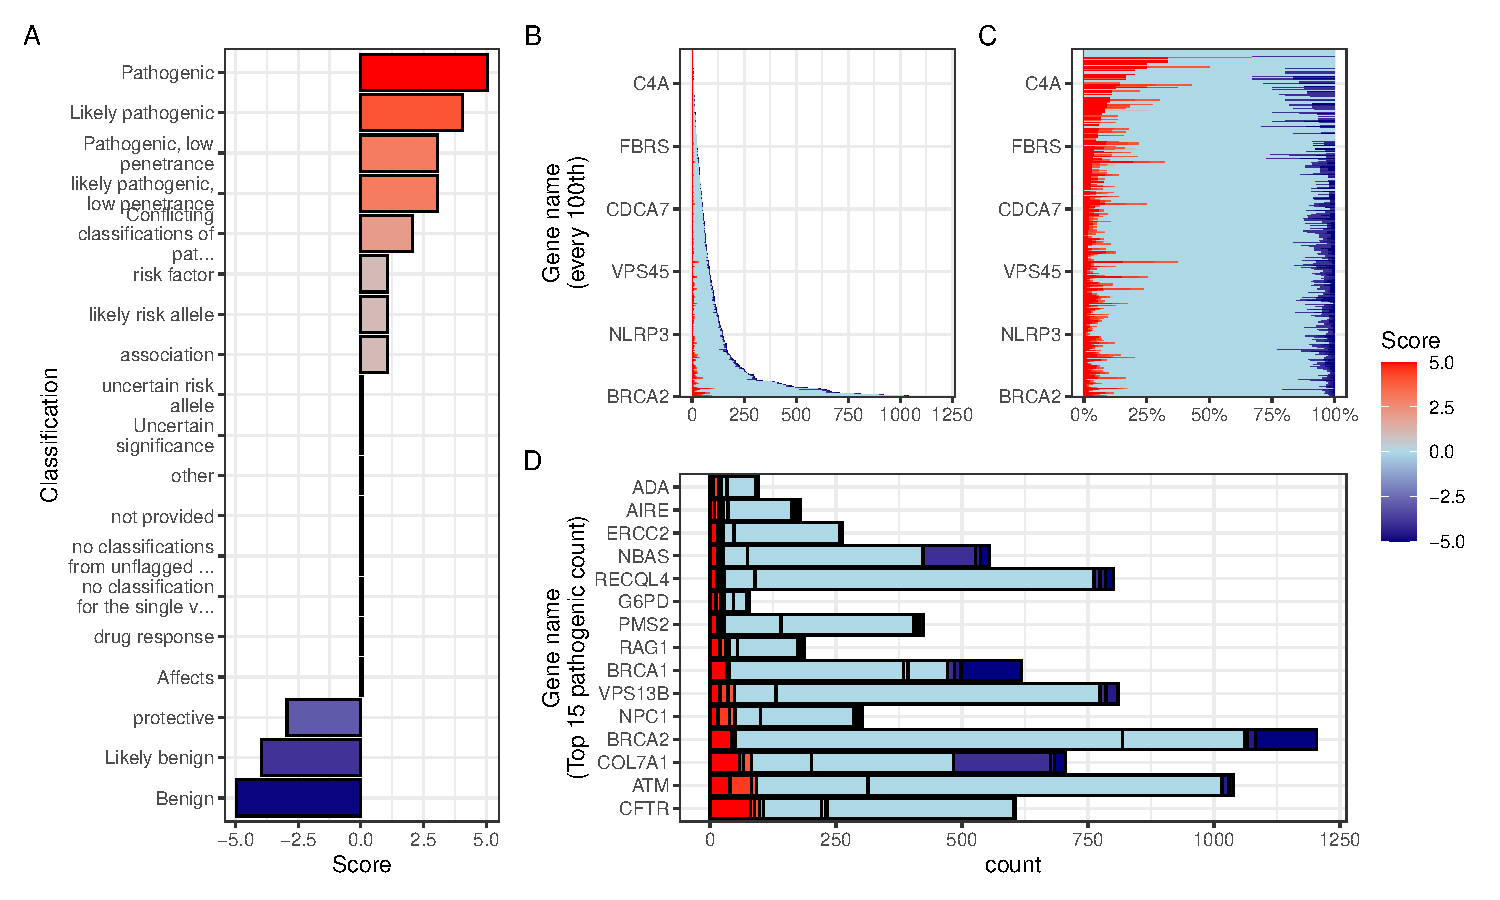
\includegraphics[width=0.99\textwidth]{../images/p_varRisEst_summary_scores.pdf}
  \caption{\textbf{Summary of ClinVar clinical significance classifications in the \ac{pid} gene panel.} (A) Shows the numeric score coding for each classification (i.e. -5 benign to +5 pathogenic) as defined in methods Section \ref{sec:classification_score}. (B) Displays the stacked absolute count of classifications per gene. The same counts are shows as percentages per gene in (C). (D) For demonstration, the top 15 genes ranked by absolute count of pathogenic (score 5) variant classifications, indicating those most frequently occurring in the population as disease-causing.
  }
  \label{fig:p_varRisEst_summary_scores}
\end{figure} 
 
\subsection{Integrating observed true positives and unobserved false negatives into a single, actionable conclusion}
\label{sec:intregrate_tp_fn}

Having established a probabilistic framework for estimating the prior probability of observing disease-associated variants under different inheritance modes, we then applied this model to an example patient to demonstrate its potential for clinical genetics.
% For each gene, we used the computed prior probabilities for all variant classifications, (e.g. benign, uncertain, and pathogenic). 
The algorithm first verified that all known pathogenic positions have been sequenced and observed as reference (true negatives), and identified any positions that were either observed as variant (true positives) or not assessable due to missing sequence data of failed \ac{qc}.
These missing sites represent potential false negatives. 
By jointly modelling the observed and unobserved space, the method yielded a calibrated, evidence-weighted probability that at least one damaging causal variant could be present within a gene.

\subsection{Scenario one - complete coverage and simple diagnosis}
We present the results from three scenarios for an example single-case patient being investigated for the genetic diagnosis of \ac{iei}.
\textbf{Figure \ref{fig:plot_scenario_1_quant_uncert_ci}} shows the results of the first simple scenario, in which only one known pathogenic variant, \ac{nfkb1} \texttt{p.Ser237Ter}, was observed and all other previously reported pathogenic positions were successfully sequenced and confirmed as reference. 
In this setting, the model assigned the full posterior probability to the observed allele, yielding 100\,\% confidence that all present evidence supported a single, true positive causal explanation. 
The most strongly supported observed variant was \texttt{p.Ser237Ter} (posterior: 0.594). 
The strongest (probability of observing) non-sequenced variant was a benign variant \texttt{p.Thr567Ile} (posterior: 0). 
The total probability of a causal diagnosis given the available evidence was 1 (95\% CI: 1--1) (\textbf{Table~\ref{tab:table_scenario_1_quant_uncert_ci}}). 

\subsection{Scenario two - incomplete coverage and complex diagnosis}

\textbf{Figure \ref{fig:plot_scenario_2_quant_uncert_ci}} shows the second more complex scenario, where the same pathogenic variant \ac{nfkb1} \texttt{p.Ser237Ter} was present, but coverage was incomplete at three additional sites of known classified variants. 
Among these was the likely-pathogenic splice-site variant \ac{nfkb1} \texttt{c.159+1G{\small\textgreater}A}, which was not captured in the sequencing data. 
The panels of \textbf{Figure \ref{fig:plot_scenario_2_quant_uncert_ci} (A–F)} illustrate the stepwise integration of observed and missing evidence, culminating in a posterior probability that reflects both confirmed findings and residual uncertainty.
\textbf{Table \ref{tab:table_scenario_2_report}} demonstrates our main goal and lists the final conclusion for reporting the clinical genetics results.
\textbf{Table \ref{tab:table_scenario_2_quant_uncert_ci}} lists the main metrics used to reach the conclusion (as illustrated in 
\textbf{Figure \ref{fig:plot_scenario_2_quant_uncert_ci}}).

Bayesian integration of every annotated allele yielded the quantitative \ac{cri}s for pathogenic attribution that (i) preserve Hardy-Weinberg expectations, (ii) accommodate \ac{ad}, \ac{ar}, \ac{xl} inheritance, and (iii) carry explicit uncertainty for non-sequenced (or failed \ac{qc}) genomic positions.  
The incremental calculation steps for the variant in question are shown in \textbf{Figure~\ref{fig:plot_scenario_2_quant_uncert_ci}}.

First, \textbf{Figure \ref{fig:plot_scenario_2_quant_uncert_ci} (A)}
depicts the prior landscape where occurrence probabilities are partitioned by observed or missing status and by causal or non‑causal evidence, with colour reflecting the underlying ClinVar score.  
\textbf{Figure \ref{fig:plot_scenario_2_quant_uncert_ci} (B)} shows posterior normalisation which concentrates probability density on two high‑confidence (high evidence score) alleles since the benign variants are, by definition, non-causal.
\textbf{Figure \ref{fig:plot_scenario_2_quant_uncert_ci} (C)} shows the resulting per‑variant probability of being simultaneously damaging and causal; only the confirmed present (true positive) nonsense variant \texttt{p.Ser237Ter} and the (false negative) hypothetical splice‑donor \texttt{c.159+1G{\small\textgreater}A} retain substantial support. 
Restricting the view to causal candidates in 
\textbf{Figure \ref{fig:plot_scenario_2_quant_uncert_ci} (D)} 
confirms that posterior mass is distributed across these two variants. 
\textbf{Figure \ref{fig:plot_scenario_2_quant_uncert_ci} (E)} decomposes the total damaging probability into observed (approximately 40\,\%) and missing (approximately 34\,\%) sources, whereas \textbf{Figure \ref{fig:plot_scenario_2_quant_uncert_ci} (F)} summarises the gene‑level posterior: inclusion of the splice‑site allele (scenario 2) produces a median probability of 0.542 with a 95\,\% \ac{cri} of 0.264–0.8. 

Numerically, the present variant \texttt{p.Ser237Ter} accounts for 0.399 of the posterior share, and the potentially causal but missing splice‑donor allele \texttt{c.159+1G{\small\textgreater}A} contributes 0.339. The remaining alleles together explain a negligible share (\textbf{Table~\ref{tab:table_scenario_2_quant_uncert_ci}}).
Thus, we can report that in this patient's scenario the probability of correct genetic diagnosis due to \ac{nfkb1} \texttt{p.Ser237Ter} is 0.542 (95 \% CrI of 0.264–0.8) given that a likely alternative remains to be confirmed for this patient.
Upon confirmation that the second variant is not present, the confidence will rise to 1 (95 \% CrI of  1–1)  as shown in scenario one.

\begin{table}[!h]
\centering
\caption{Final variant report for clinical genetics scenario 2. Reported causal: \texttt{p.Ser237Ter} (posterior 0.377). Undetected causal: \texttt{c.159+1G>A} (posterior 0.364). The total probability of a causal diagnosis given the available evidence was 0.511 (95\% CI: 0.237--0.774).\label{tab:table_scenario_2_report}}
\centering
\resizebox{\ifdim\width>\linewidth\linewidth\else\width\fi}{!}{
\begin{tabular}[t]{>{\raggedright\arraybackslash}p{4cm}>{\raggedright\arraybackslash}p{6cm}>{\raggedright\arraybackslash}p{6cm}}
\toprule
Parameter & present & missing\\
\midrule
Gene & NFKB1 & NFKB1\\
HGVSc & c.710C>G & c.159+1G>A\\
HGVSp & p.Ser237Ter & .\\
Inheritance & AD & AD\\
Patient sex & Male & Male\\
gnomAD frequency & 6.57e-06 & 6.57e-06\\
95\% CI lower & 0.003 & NA\\
p(median) & 0.090 & NA\\
95\% CI upper & 0.551 & NA\\
Posterior p(causal) & 0.377 & 0.364\\
Interpretation & Reported causal; variant observed & Reported causal; variant not detected — consider follow‑up\\
\midrule
\textbf{Summary} & \multicolumn{2}{p{10cm}}{Overall probability of correct causal diagnosis due to SNV/INDEL given the currently available evidence: 0.511 (95\% CI 0.237--0.774). } \\
\bottomrule
\end{tabular}}
\end{table}


\FloatBarrier
\subsection{Scenario three - currently impossible diagnosis}

\textbf{Figure~\ref{fig:plot_scenario_3_quant_uncert_ci}} shows the third scenario, in which no observed variants were detected in the proband for \ac{nfkb1}. 
Instead, a broad range of plausible \ac{fn} were detected as missing for the gene \ac{tnfaip3}.
The strongest (probability of observing and pathogenic) of these non-sequenced variants was \texttt{p.Cys243Arg} (posterior: 0.347). 
However, the total probability of a causal diagnosis for the patient \emph{given the available evidence} was 0 (95\% CI: 0--0) since these missing variants must be accounted for (\textbf{Table~\ref{tab:table_scenario_3_quant_uncert_ci}}). 
Upon confirmation, these probabilities can update, as per scenario two.

\subsection{Posterior probabilities are calculated across all qualifying variants}

While only the top-ranked gene/variant is shown in each of the three scenarios, we emphasise that the same posterior probability and \ac{cri} calculations are performed across all plausible candidates. 
In real-world diagnostics, we commonly find multiple variants to carry non-negligible probabilities. 
Our framework explicitly quantifies these competing hypotheses, enabling a ranked interpretation that reflects the totality of evidence. 
Overlapping \ac{cri} do not indicate ambiguity in the method, but rather a principled measure of remaining uncertainty. 
This output can directly inform follow-up actions, such as functional validation or treatment trials, and supports the use of CrI thresholds as a transparent decision-making aid when data are incomplete or equivocal.

\begin{figure}[ht]
  \centering
  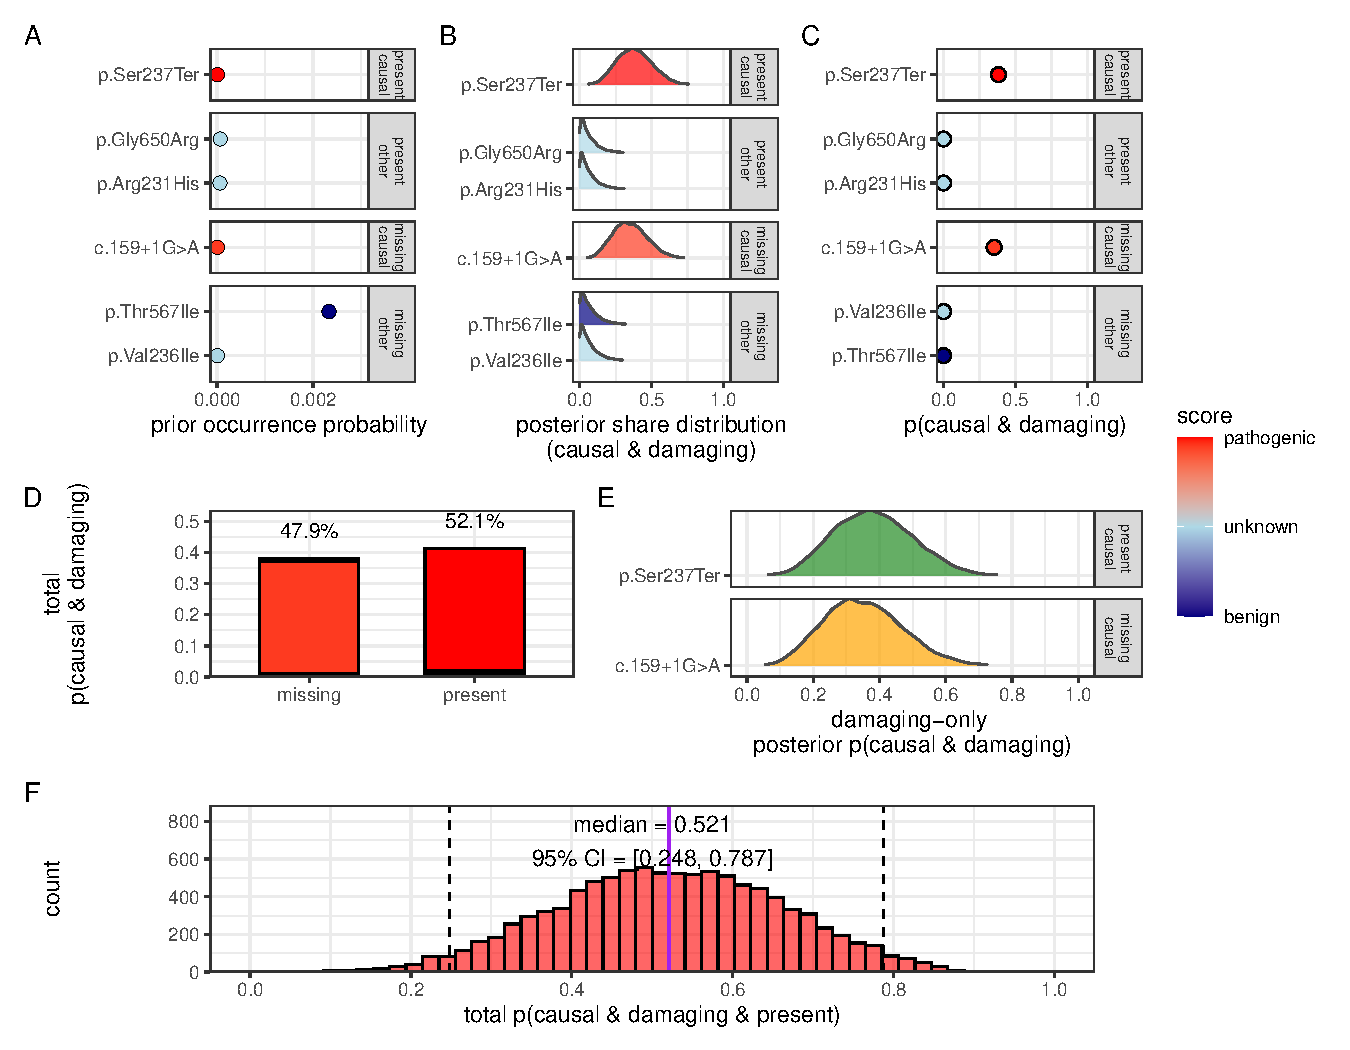
\includegraphics[width=0.99\textwidth]{../images/plot_scenario_2_quant_uncert_ci.pdf}
  \caption{
    \textbf{Quantification of present (\ac{tp}) and missing (\ac{fn}) causal genetic variants for disease in \textit{NFKB1} (scenario 2).}
    The example proband carried three known heterozygous variants, including pathogenic \texttt{p.Ser237Ter}, and had incomplete coverage at three additional loci, including likely-pathogenic splice-site variant \texttt{c.159+1G{\small\textgreater}A}.  The sequential steps towards the posterior  probability of complete genetic diagnosis are shown:
    (A) Prior occurrence probabilities, stratified by observed/missing and causal/non-causal status. Pathogenicity scores (-5 to +5) are annotated.
    (B) Posterior distributions of normalised variant weights \(\tilde{\pi}_i\).  
    (C) Per-variant posterior probability of being both damaging and causal.  
    (D) Posterior distributions for causal variants only.  
    (E) Decomposition of total pathogenic probability into observed (green) and missing (orange) sources.  
    (F) Gene-level posterior showing the probability that at least one damaging causal allele is present; median 0.54, 95\,\% \ac{cri} 0.26-0.80. This result can be compared to scenarios one and three in 
    \textbf{Figures \ref{fig:plot_scenario_1_quant_uncert_ci}} and
    \textbf{\ref{fig:plot_scenario_3_quant_uncert_ci}}, respectively.
  }
  \label{fig:plot_scenario_2_quant_uncert_ci}
\end{figure}

\FloatBarrier
\subsection{Validation studies}
\subsubsection{Validation of dominant disease occurrence with \textit{NFKB1}}

To validate our genome-wide probability estimates for \ac{ad} disorders, we focused on \ac{nfkb1}.
We used a reference dataset from \citet{tuijnenburgNFKB12018}, in which whole-genome sequencing of 846 \ac{pid} patients identified \ac{nfkb1} as one of the genes most strongly associated with the disease, with 16 \ac{nfkb1}-related \ac{cvid} cases attributed to \ac{ad} heterozygous variants. 
Our goal was to compare the predicted number of \ac{nfkb1}-related \ac{cvid} cases with the reported count in this well-characterised national-scale cohort.

Our model calculated 0 known pathogenic variant \ac{nfkb1}-related \ac{cvid} cases in the UK with a minimal risk of 456 unknown de novo variants. In the reference cohort, 16 \ac{nfkb1} \ac{cvid} cases were reported. 
We additionally wanted to account for potential under-reporting in the reference study. 
We used an extrapolated national \ac{cvid} prevalence which yielded a median estimate of 118 cases (95\% CI: 70–181), while a Bayesian-adjusted mixture estimate produced a median of 67 cases (95\% CI: 43–99). \textbf{Figure \ref{fig:validation_studies_bayesian_adjusted_estimates} (A)} illustrates that our predicted values reflect these ranges and are closer to the observed count. 
This case supports the validity of our integrated probability estimation framework for \ac{ad} disorders, and represents a challenging example where pathogenic \ac{snv} are not reported in the reference population of gnomAD. Our min-max values successfully contained the true reported values.


\subsubsection{Validation of recessive disease occurrence with \textit{CFTR}}

Our analysis predicted the number of \ac{cf} cases attributable to carriage of the \texttt{p.Arg117His} variant (either as homozygous or as compound heterozygous with another pathogenic allele) in the UK. Based on \ac{hwe} calculations and mortality adjustments, we predicted approximately 648 cases arising from biallelic variants and 160 cases from homozygous variants, resulting in a total of 808 expected cases.

In contrast, the nationally reported number of \ac{cf} cases was 714, as recorded in the UK Cystic Fibrosis Registry 2023 Annual Data Report
\cite{naito2023uk}. To account for factors such as reduced penetrance and the mortality-adjusted expected genotype, we derived a Bayesian-adjusted estimate via posterior simulation. Our Bayesian approach yielded a median estimate of 740 cases (95\% \ac{ci}: 696, 786) and a mixture-based estimate of 727 cases (95\% \ac{ci}: 705, 750).
\textbf{Figure \ref{fig:validation_studies_bayesian_adjusted_estimates} (B)} illustrates the close concordance between the predicted values, the Bayesian-adjusted estimates, and the national report supports the validity of our approach for estimating disease.


\textbf{Figure \ref{fig:validation_scatter_dense}} shows the final values for these genes of interest in a given population size and phenotype. It reveals that an allele frequency threshold of approximately 0.000007 is required to observe a single heterozygous carrier of a disease-causing variant in the UK population for both genes. However, owing to the \ac{ar} \ac{moi} pattern of \ac{cftr}, this threshold translates into more than 100,000 heterozygous carriers, compared to only 456 carriers for the \ac{ad} gene \ac{nfkb1}. Note that this allele frequency threshold, being derived from the current reference population, represents a lower bound that can become more precise as public datasets continue to grow. This marked difference underscores the significant impact of \ac{moi} patterns on population carrier frequencies and the observed disease prevalence.

\FloatBarrier
\subsubsection{Interpretation of ClinVar variant occurrences}

\textbf{Figure~\ref{fig:all_genes_combined_bar_charts_mini}} shows  the two validation study \ac{pid} genes, representing \ac{ar} and dominant \ac{moi}. \textbf{Figure~\ref{fig:all_genes_combined_bar_charts_mini} (A)}   illustrates the overall probability of an affected birth by ClinVar variant classification, whereas \textbf{Figure~\ref{fig:all_genes_combined_bar_charts_mini}  (B)}  depicts the total expected number of cases per classification for an example population, here the UK, of approximately 69.4 million. 

\subsubsection{Validation of SCID-specific disease occurrence}

Given that \ac{scid} is a subset of \ac{pid}, our probability estimates reflect the likelihood of observing a genetic variant as a diagnosis when the phenotype is \ac{pid}. 
However, we additionally tested our results against \ac{scid} cohorts in 
 \textbf{Figure \ref{fig:scid_combined}}.
The summarised raw cohort data for SCID-specific gene counts are summarised and compared across countries in \textbf{Figure \ref{fig:scid_gene_comparison}}.
True counts for \textit{IL2RG} and \ac{dclre1c} from ten distinct locations yielded 95\% \ac{ci} surrounding our predicted values. 
For \ac{il2rg}, the prediction was low (approximately 1 case per 1,000,000 \ac{pid}), as expected since loss-of-function variants in this \ac{xl} gene are highly deleterious and rarely observed in gnomAD. In contrast, the predicted value for \ac{rag1} was substantially higher (553 cases per 1,000,000 \ac{pid}) than the observed counts (ranging from 0 to 200). 
We attributed this discrepancy to the lower penetrance and higher background frequency of \ac{rag1} variants in recessive inheritance, whereby reference studies may underreport the true national incidence. 
Overall, we report that agreement within an order of magnitude was tolerable given the inherent uncertainties from reference studies arising from variable penetrance and allele frequencies.

\FloatBarrier
\subsection{Application in inborn errors of immunity}
\subsection{Genetic constraint in high-impact protein networks}

Sean- In this section I was lost. I don't see the connection to the previous sections, or how it relates to the original goals.

Dylan - I need an introduction here with reasoning to show that instead of focusing on every IEI gene individually, we can cluster them based on protein networks and phenotypes, thereby increasing the value of the traditional IUIS IEI classification. 



We next examined genetic constraint in high-impact protein networks across the whole \ac{iei} gene set of over 500 known disease-gene phenotypes \cite{poli_human_2025}. By integrating ClinVar variant classification scores with \ac{ppi} data, we quantified the pathogenic burden per gene and assessed its relationship with network connectivity and genetic constraint
\cite{szklarczyk2025string, karczewski2020mutational}.

\subsubsection{Score-positive-total within IEI PPI network}

The ClinVar classifications reported in 
\textbf{Figure \ref{fig:p_varRisEst_summary_scores}} were scaled -5 to +5 based on their pathogenicity. 
We were interested in positive (potentially damaging) but not negative (benign) scoring variants, which are statistically incidental in this analysis. 
We tallied gene-level positive scores to give the score-positive-total metric. 
\textbf{Figure \ref{fig:ppi_network_assoc} (A)} shows the \ac{ppi} network of disease-associated genes, where node size and colour encode the score-positive-total (log-transformed). 
The top 15 genes with the highest total prior probabilities of being observed with disease are labelled (as per \textbf{Figure \ref{fig:p_varRisEst_summary_scores}}).


\FloatBarrier
\subsubsection{Association analysis of score-positive-total across IEI categories} 

We checked for any statistical enrichment in score-positive-totals, which represents the expected observation of pathogenicity, between the \ac{iei} categories.
One-way \ac{anova} revealed an effect of major disease category on score-positive-total (\(F(8,500)=2.82,\,p=0.0046\)), indicating that group means were not identical, which we observed in
\textbf{Figure \ref{fig:ppi_network_assoc} (B)}.
However, despite some apparent differences in median scores across categories (i.e. 9. \ac{bmf}), the Tukey \ac{hsd} post hoc comparisons 
\textbf{Figure \ref{fig:ppi_network_assoc} (C)}
showed that all pairwise differences had 95\% \ac{ci}s overlapping zero, suggesting that individual group differences were not significant.

\FloatBarrier
\subsubsection{UMAP embedding of the PPI  network}
To address the density of the \ac{ppi} network for the \ac{iei} gene panel, we applied \ac{umap} (\textbf{Figure \ref{fig:p_umap}}). 
Node sizes reflect interaction degree, a measure of evidence-supported connectivity \cite{szklarczyk2025string}. We tested for a correlation between interaction degree and score-positive-total. In \textbf{Figure \ref{fig:p_umap}}, gene names with degrees above the 95th percentile are labelled in blue, while the top 15 genes by score-positive-total are labelled in yellow (as per \textbf{Figure \ref{fig:p_varRisEst_summary_scores}}). Notably, genes with high pathogenic variant loads segregated from highly connected nodes, suggesting that \ac{lof} in hub genes is selectively constrained, whereas damaging variants in lower-degree genes yield more specific effects. 
This observation was subsequently tested empirically.

\begin{figure}[ht]
  \centering
  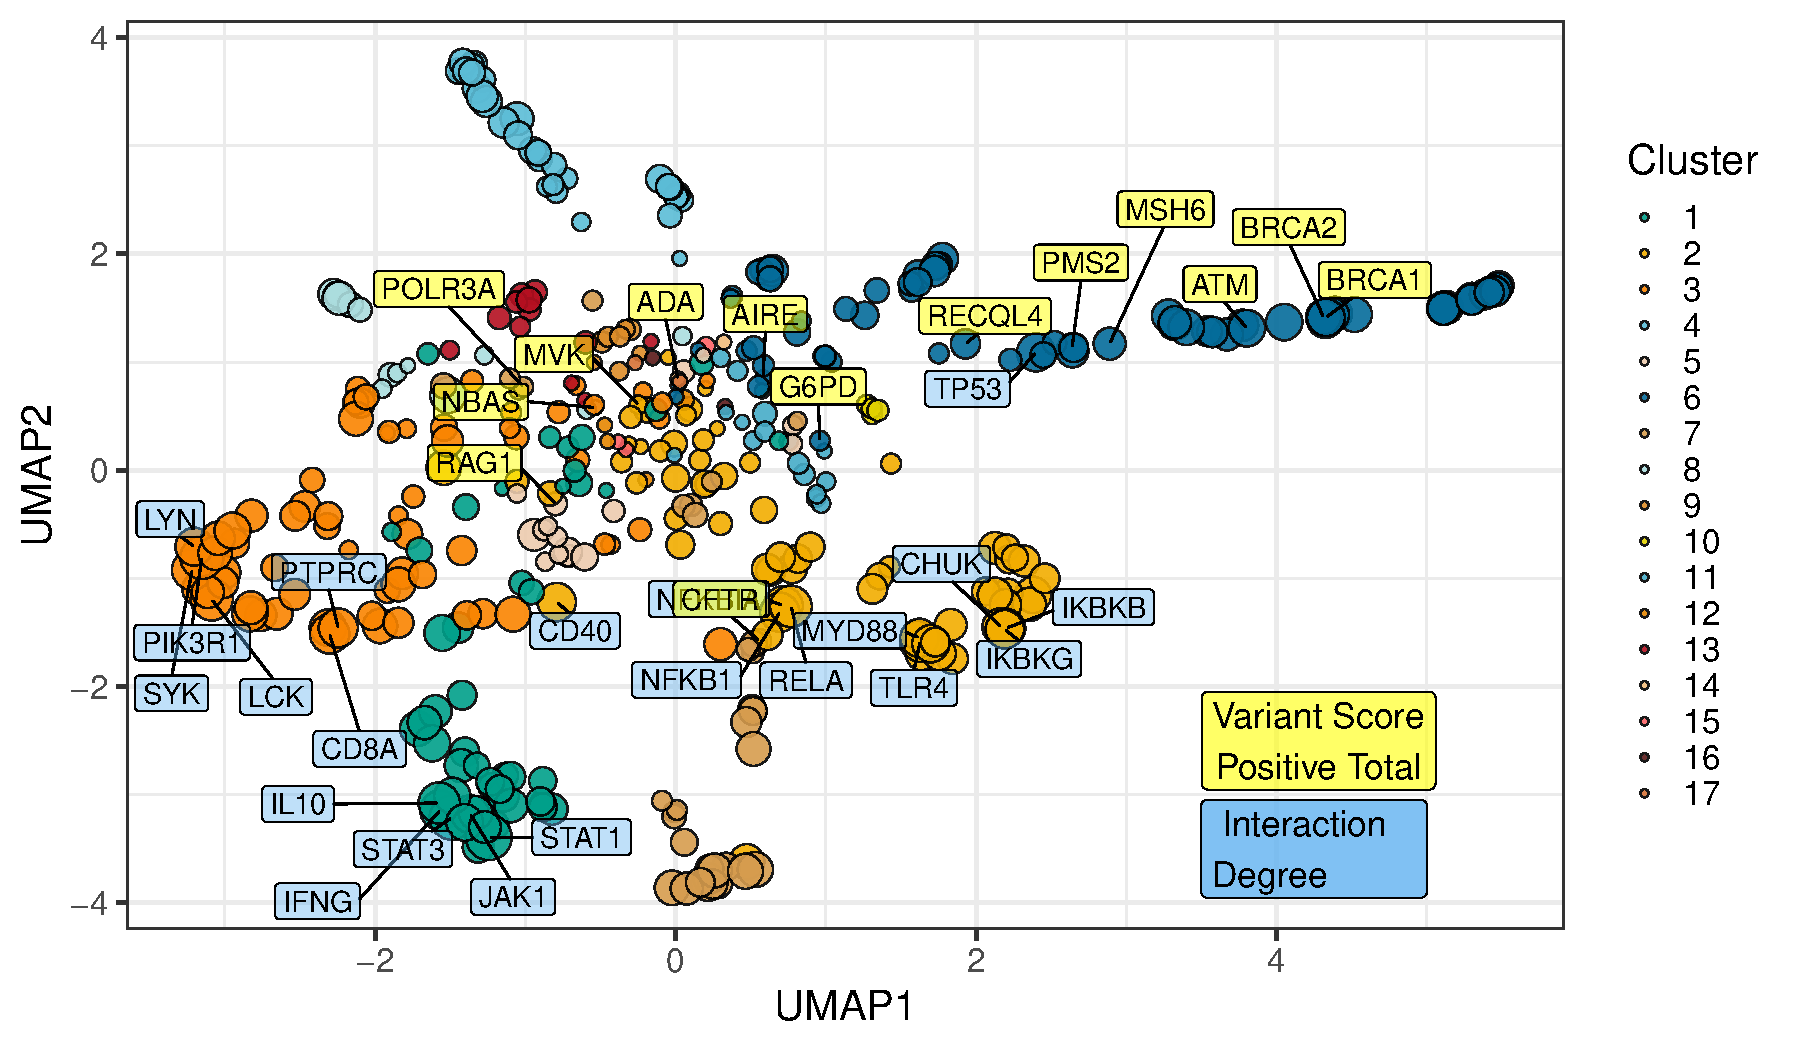
\includegraphics[width=0.99\textwidth]{../images/untangleR_ppi_network_umap.pdf}
  \caption{
    \textbf{\ac{umap} embedding of the \ac{ppi} network.} 
    The plot projects the high-dimensional protein-protein interaction network into two dimensions, with nodes coloured by cluster and sized by interaction degree. Blue labels indicate hub genes (degree above the 95th percentile) and yellow labels mark the top 15 genes by score-positive-total (damaging ClinVar classifications). The spatial segregation suggests that genes with high pathogenic variant loads are distinct from highly connected nodes.
  }
  \label{fig:p_umap}
\end{figure}

\FloatBarrier
\subsubsection{Hierarchical clustering of enrichment scores for major disease categories}
\textbf{Figure \ref{fig:patch2}} presents a heatmap of standardised residuals for major disease categories across network clusters, as per \textbf{Figure \ref{fig:p_umap}}. 
A dendrogram clusters similar disease categories, while the accompanying bar plot displays the maximum absolute standardised residual for each category.
Notably, (8) \ac{cd} shows the highest maximum enrichment, followed by 
(9) \ac{bmf}. 
While all maximum values exceed 2, the threshold for significance, this likely reflects the presence of protein clusters with strong damaging variant scores rather than uniform significance across all categories (i.e. genes from cluster 4 in 8 \ac{cd}).


\subsubsection{PPI connectivity, LOEUF constraint and enriched network cluster analysis}

Based on the preliminary insight from \textbf{Figure \ref{fig:patch2}},
we evaluated the relationship between network connectivity (\ac{ppi} degree) and \ac{lof} constraint (\ac{loeuf} upper rank) \citet{karczewski2020mutational} using Spearman’s rank correlation.
Overall, there was a weak but significant negative correlation ($\rho = -0.181$, $p = 0.00024$) at the global scale, indicating that highly connected genes tend to be more constrained. 
A supplementary analysis (\textbf{Figure \ref{fig:p_umap_const}})
did not reveal distinct visual associations between network clusters and constraint metrics, likely due to the high network density. 
However once stratified by gene clusters, the natural biological scenario based on quantitative \ac{ppi} evidence \cite{szklarczyk2025string},
some groups showed strong correlations; for instance, cluster 2 ($\rho = -0.375$, $p = 0.000994$) and cluster 4 ($\rho = -0.800$, $p < 0.000001$), while others did not.
This indicated that shared mechanisms within pathway clusters may underpin genetic constraints, particularity for \ac{lof} intolerance. We observe that the score-positive-total metric effectively summarises the aggregate pathogenic burden across \ac{iei} genes, serving as a robust indicator of genetic constraint and highlighting those with elevated disease relevance.


% \subsubsection{Network Analysis of Enriched Significant Clusters Based on \ac{gnomad} Constraint}
\textbf{Figure \ref{fig:p_cor_spear_rho_sig_clust_patch3} (C, D)} shows the re-plotted \ac{ppi} networks for clusters with significant correlations between \ac{ppi} degree and \ac{loeuf} upper rank. In these networks, node size is scaled by a normalised variant score, while node colour reflects the variant score according to a predefined palette.

\subsection{New insight from functional enrichment}
To interpret the functional relevance of our prioritised \ac{iei} gene sets with the highest load of damaging variants (i.e. clusters 2 and 4 in \textbf{Figure \ref{fig:p_cor_spear_rho_sig_clust_patch3}}), we performed functional enrichment analysis for known disease associations using MsigDB with FUMA (i.e. GWAScatalog and Immunologic Signatures) \cite{watanabe_functional_2017}. Composite enrichment profiles (\textbf{Figure \ref{fig:fuma_merge}}) reveal that our enriched \ac{ppi} clusters were associated with distinct disease-related phenotypes, providing functional insights beyond traditional \ac{iuis} \ac{iei} groupings \cite{poli_human_2025}. The gene expression profiles shown in \textbf{Figure \ref{fig:expHeatmaps}} (GTEx v8 54 tissue types) offer the tissue-specific context for these associations. Together, these results enable the annotation of \ac{iei} gene sets with established disease phenotypes, supporting a data-driven classification of \ac{iei}.

Based on these independent sources of interpretation, we observed that genes from cluster 2 were independently associated with specific inflammatory phenotypes, including ankylosing spondylitis, psoriasis, inflammatory bowel disease, and rheumatoid arthritis, as well as quantitative immune traits such as lymphocyte and neutrophil percentages and serum protein levels.
In contrast, genes from cluster 4 were linked to ocular and complement-related phenotypes, notably various forms of age-related macular degeneration (e.g. geographic atrophy and choroidal neovascularisation) and biomarkers of the complement system (e.g. C3, C4, and factor H-related proteins), with additional associations to nephropathy and pulmonary function metrics.

\subsection{Genome-wide gene distribution and linkage disequilibrium}

\textbf{Figure \ref{fig:karyo_locusplot_merged} (A)} shows a genome-wide karyoplot of all \ac{iei} panel genes across GRCh38, with colour-coding based on \ac{moi}. Figures \textbf{(B)} and \textbf{(C)} display zoomed-in locus plots for \textit{NFKB1} and \textit{CFTR}, respectively. 
In \textbf{Figure \ref{fig:karyo_locusplot_merged} (B)}, the probability of observing variants with known classifications is high only for variants such as p.Ala475Gly, which are considered benign in the \ac{ad} \textit{NFKB1} gene that is intolerant to \ac{lof}. 
In \textbf{Figure \ref{fig:karyo_locusplot_merged} (C)}, high probabilities of observing patients with pathogenic variants in \textit{CFTR} are evident, reproducing this well-established phenomenon. Furthermore, the analysis of \ac{ld} using $\text{R}^2$ shows that high LD regions can be modelled effectively, allowing independent variant signals to be distinguished.

\begin{figure}[ht]
  \centering
  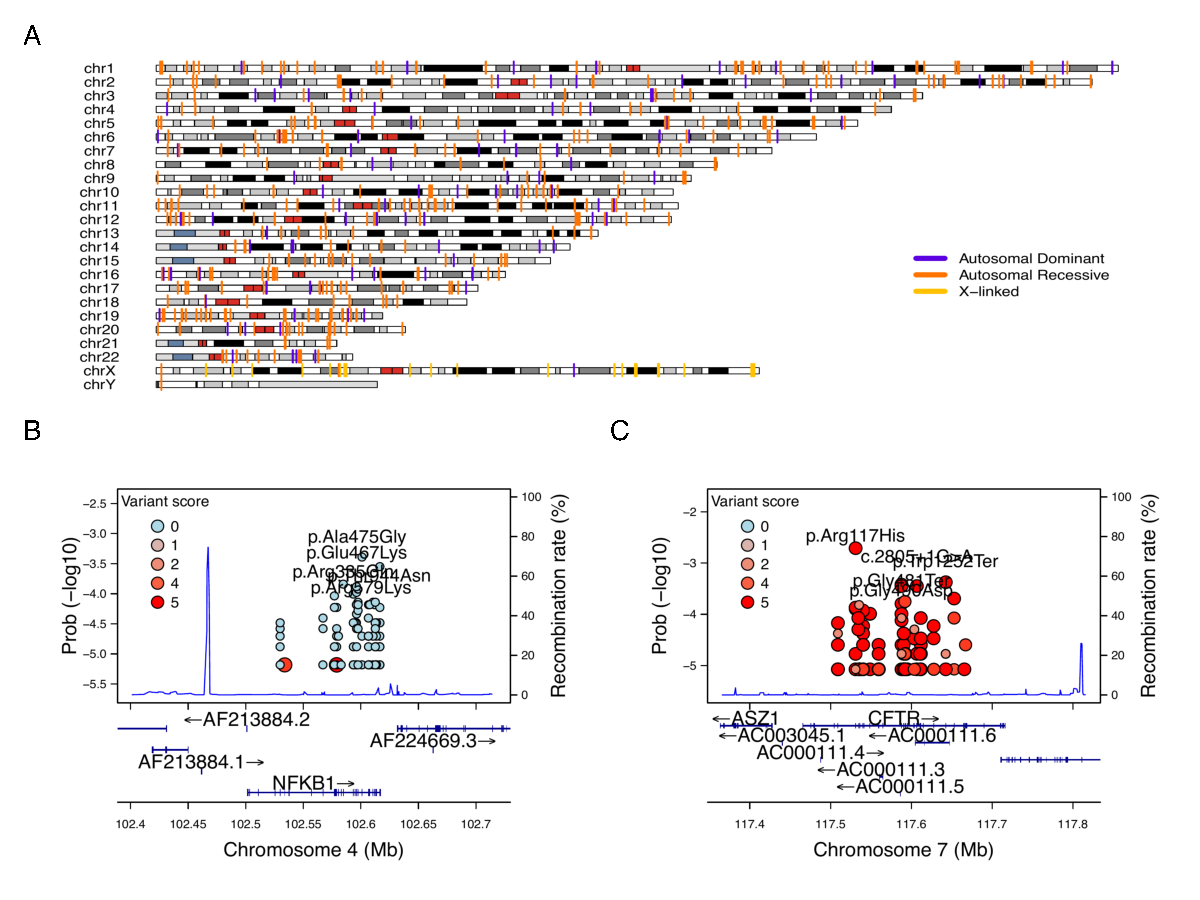
\includegraphics[width=0.99\textwidth]{../images/karyo_locusplot_merged.pdf}
  \caption{\textbf{Genome-wide \ac{iei}, variant occurrence probability and \ac{ld} by $\text{R}^2$.} (A) Genome-wide karyoplot of all \ac{iei} panel genes mapped to GRCh38, with colours indicating \ac{moi}. (B) Zoomed-in locus plot example for \textit{NFKB1} showing variant occurrence probabilities; only benign variants such exhibit high probabilities in this \ac{ad} gene intolerant to \ac{lof}. (C) Locus plot example for \textit{CFTR} displaying high probabilities for pathogenic variants; due to the dense clustering of pathogenic variants, score filter >0 was applied. Top five variants are labelled per gene.}
  \label{fig:karyo_locusplot_merged}
\end{figure}

\FloatBarrier
\subsection{Novel PID classifications derived from genetic PPI and clinical features}
We recategorised 315 immunophenotypic features from the original \ac{iuis} \ac{iei} annotations, reducing detailed descriptions (e.g.\ “decreased CD8, normal or decreased CD4”) to minimal labels (e.g.\ “low”) and then binarising them (normal vs.\ not-normal) for T cells, B cells, \ac{ig} and neutrophils 
(\textbf{Figure \ref{fig:immunophenotype_before_after}}). 
These simplified profiles were mapped onto STRINGdb \ac{ppi} clusters, revealing non‑random distributions ($\chi^2 < 1e‑13$; 
\textbf{Figure \ref{fig:plot_multicat_patch_3_clust_chi}}), indicating that network context captures key immunophenotypic variation.

We next compared four classifiers under 5‑fold cross‑validation to determine which features predicted \ac{ppi} clustering.
As shown in \textbf{Figure \ref{fig:multicat_performance_combined}}, the fully combined model achieved the highest accuracy among the four:
(i) phenotypes only (33 \%) (i.e. T cell, B cell, \ac{ig}, Neutrophil);
(ii) phenotypes + IUIS major category (50 \%) (e.g. CID. See \textbf{Box \ref{box:definitions}} for more);
(iii) \ac{iuis} major + subcategory only (59 \%) (e.g. CID, T-B+ SCID); and
(iv) phenotypes + IUIS major + subcategory  (61 \%).
This demonstrated that incorporating both traditional \ac{iuis} \ac{iei} classifications and core immunophenotypic markers into the \ac{ppi}‑based framework yielded the most robust discrimination of \ac{pid} gene clusters.
Variable importance analysis highlighted abnormality status for \ac{ig} and T cells
were among the top ten features in addition to the other \ac{iuis} major and sub categories. 
Per‑class specificity remained uniform across the classes while sensitivity dropped.

The \ac{ppi}  and  immunophenotype model yielded 17 data‑driven PID groups, whereas incorporating the full complement of \ac{iuis} categories expanded this to 33 groups. 
For clarity, we only demonstrate the decision tree from the smaller 17‑group model in 
\textbf{Figure \ref{fig:pid_class_tree_distribution}}.
% full model: plot_multicat_combined_classification_tree.pdf
Each terminal node is annotated by its predominant immunophenotypic signature (for example, ``group 65 with abnormal T cell and B cell features''), and the full resulting gene counts per 33 class are plotted in 
% \textbf{Figure \ref{fig:multicat_new_pid_classes_combined}}. 
\textbf{Figure \ref{fig:pid_class_tree_distribution}}.
Although, less user-friendly, this data‑driven taxonomy 
both aligns with and refines traditional \ac{iuis} \ac{iei} classifications
%Although, less user-friendly, 
to provide a scaffold for large‑scale computational analyses.
Because this framework is fully reproducible, alternative \ac{ppi} embeddings that incorporate additional molecular annotations can readily swapped to continue building on these \ac{iei} classification schemes.

\begin{figure}[ht]
  \centering
  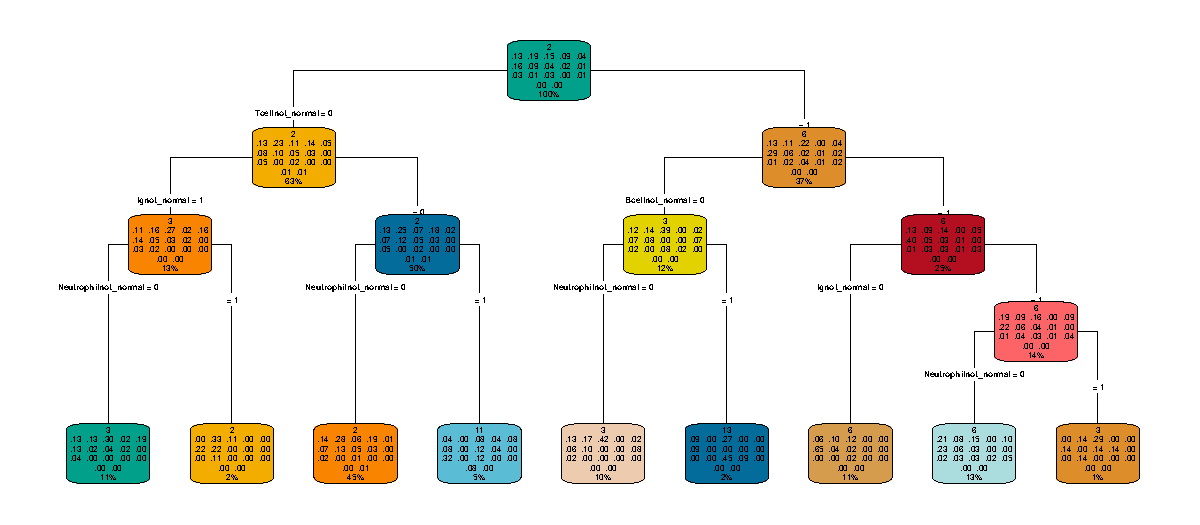
\includegraphics[width=0.99\textwidth]{../images/p_new_classification_finetune_tree.pdf}       
  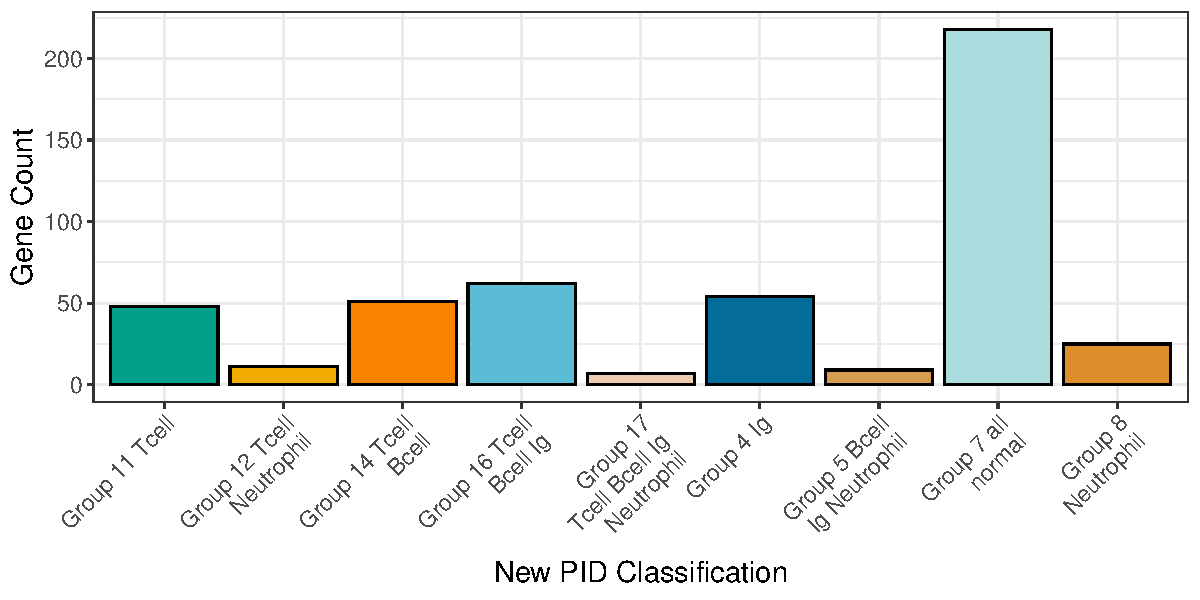
\includegraphics[width=0.99\textwidth]{../images/plot_new_pid_classifications_genetic.pdf}
  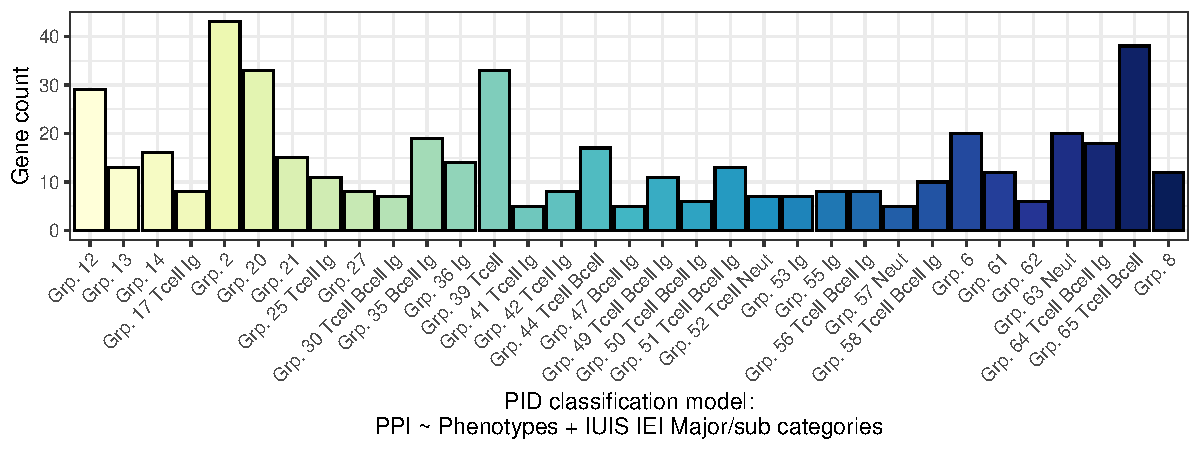
\includegraphics[width=0.99\textwidth]{../images/plot_multicat_new_pid_classes_combined.pdf}
  \caption{\textbf{ Fine-tuned model for PID classification.} 
  (Top) In each terminal node, the top block indicates the number of genes in the node; the middle block shows the fitted class probabilities (which sum to 1); and the bottom block displays the percentage of the total sample in that node. These metrics summarise the model's assignment based on immunophenotypic and \ac{ppi} features. (Middle) Bar plot presenting the distribution of novel PID classifications, where group labels denote the predominant abnormal clinical feature(s) (e.g. T cell, B cell, Ig, Neutrophil) characterising each group. (Bottom) The complete model including the traditional \ac{iuis} \ac{iei} categories.}  
  \label{fig:pid_class_tree_distribution}
\end{figure}

\FloatBarrier
\subsection{Probability of observing AlphaMissense pathogenicity}
AlphaMissense provides pathogenicity scores for all possible amino acid substitutions; however, our results in \textbf{Figure \ref{fig:alphamissense}} show that the most probable observations in patients occur predominantly for benign or unknown variants. This finding places the likelihood of disease-associated substitutions into perspective and offers a data-driven foundation for future improvements in variant prediction. The values in 
\textbf{Figure \ref{fig:alphamissense} (A)} can be directly compared to 
\textbf{Figure \ref{fig:p_varRisEst_summary_scores} (D)} to view the distribution of classifications.
A Kruskal-Wallis test was used to compare the observed disease probability across clinical classification groups and no significant differences were detected. In general, most variants in patients are classified as benign or unknown, indicating limited discriminative power in the current classification, such that pathogenicity prediction does not infer occurrence prediction (\textbf{Figure \ref{fig:alphamissense_kw}}).
Inverse correlation likely depends on factors like \ac{moi} and intolerance to \ac{lof}.
  
\begin{figure}[ht]
\begin{center}
%    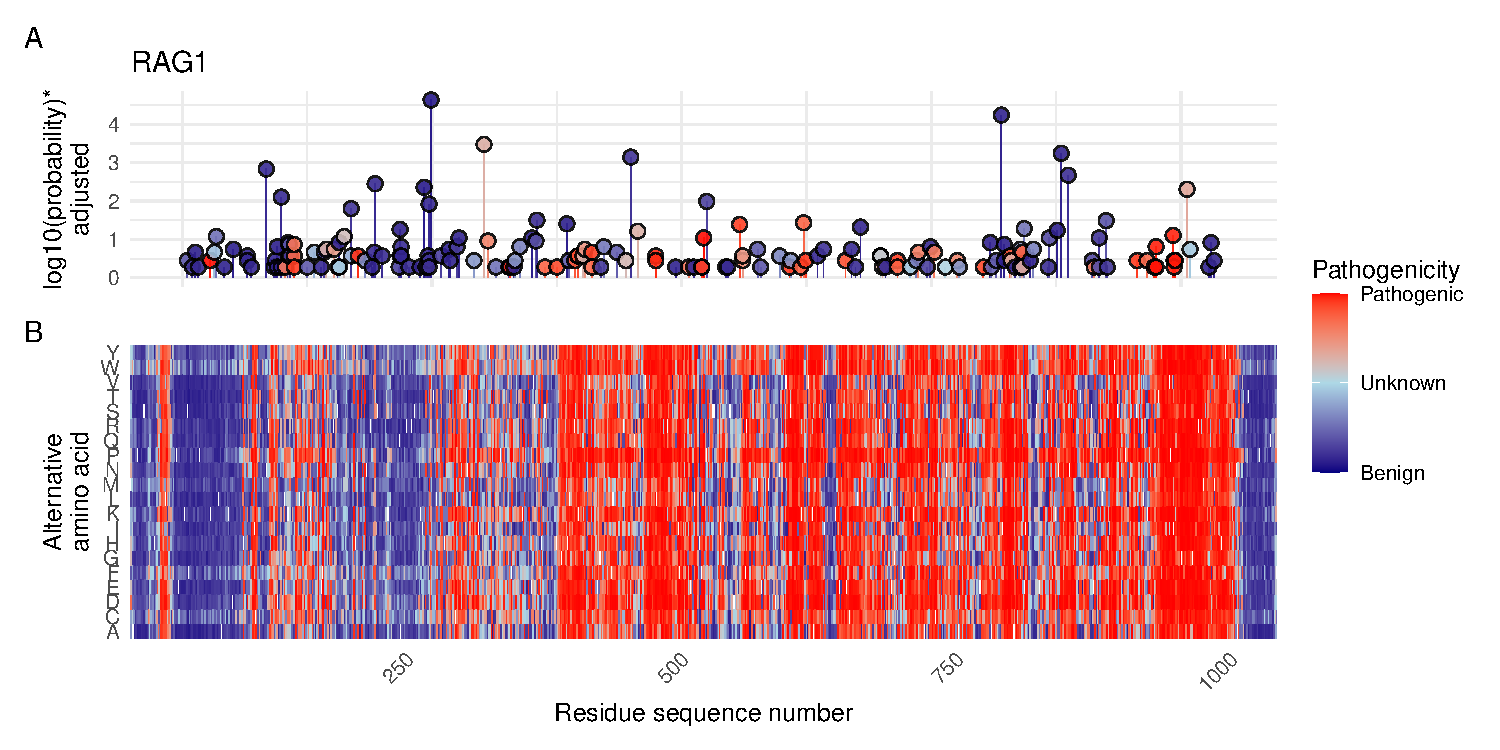
\includegraphics[width=0.99\textwidth]{../images/p_alphamissense_RAG1.pdf}
    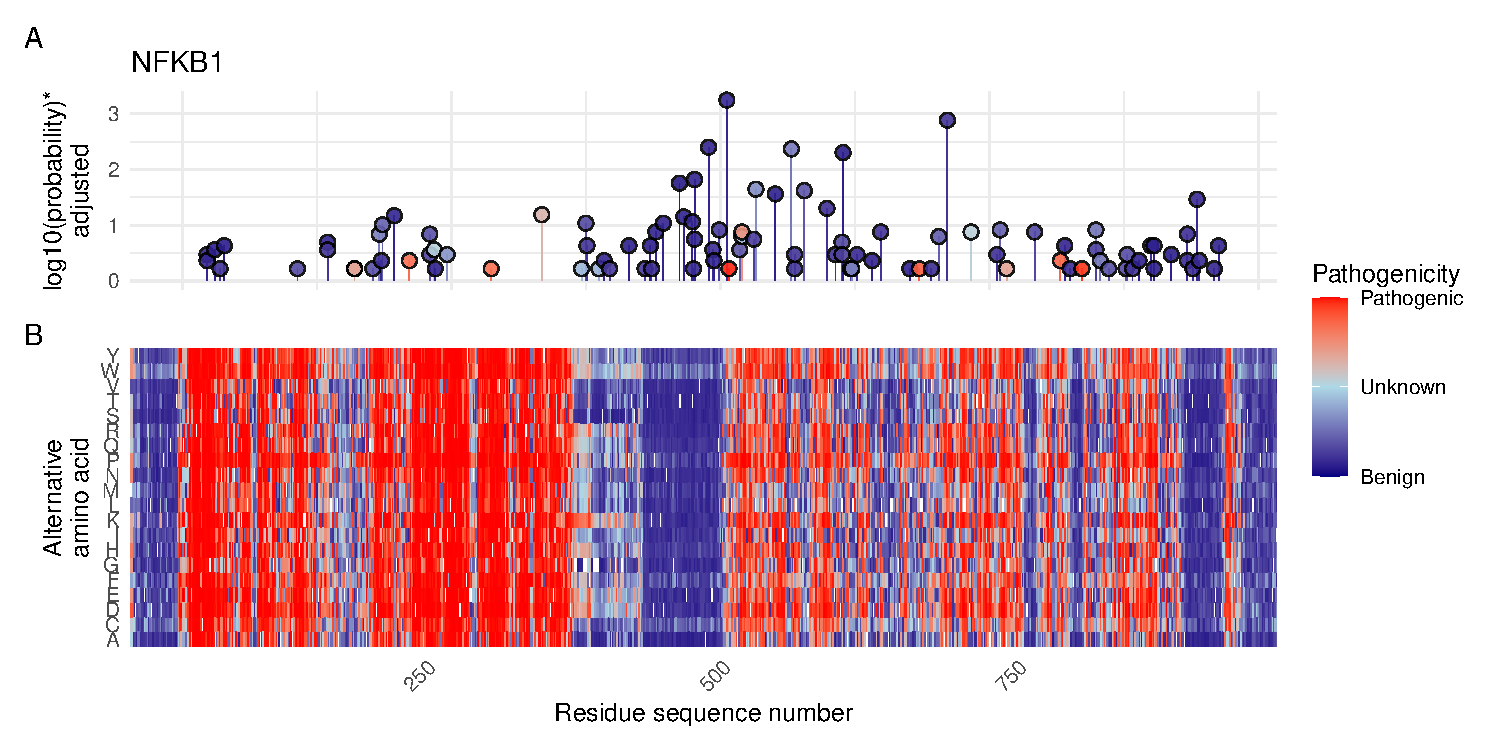
\includegraphics[width=0.8\textwidth]{../images/p_alphamissense_NFKB1.pdf}
    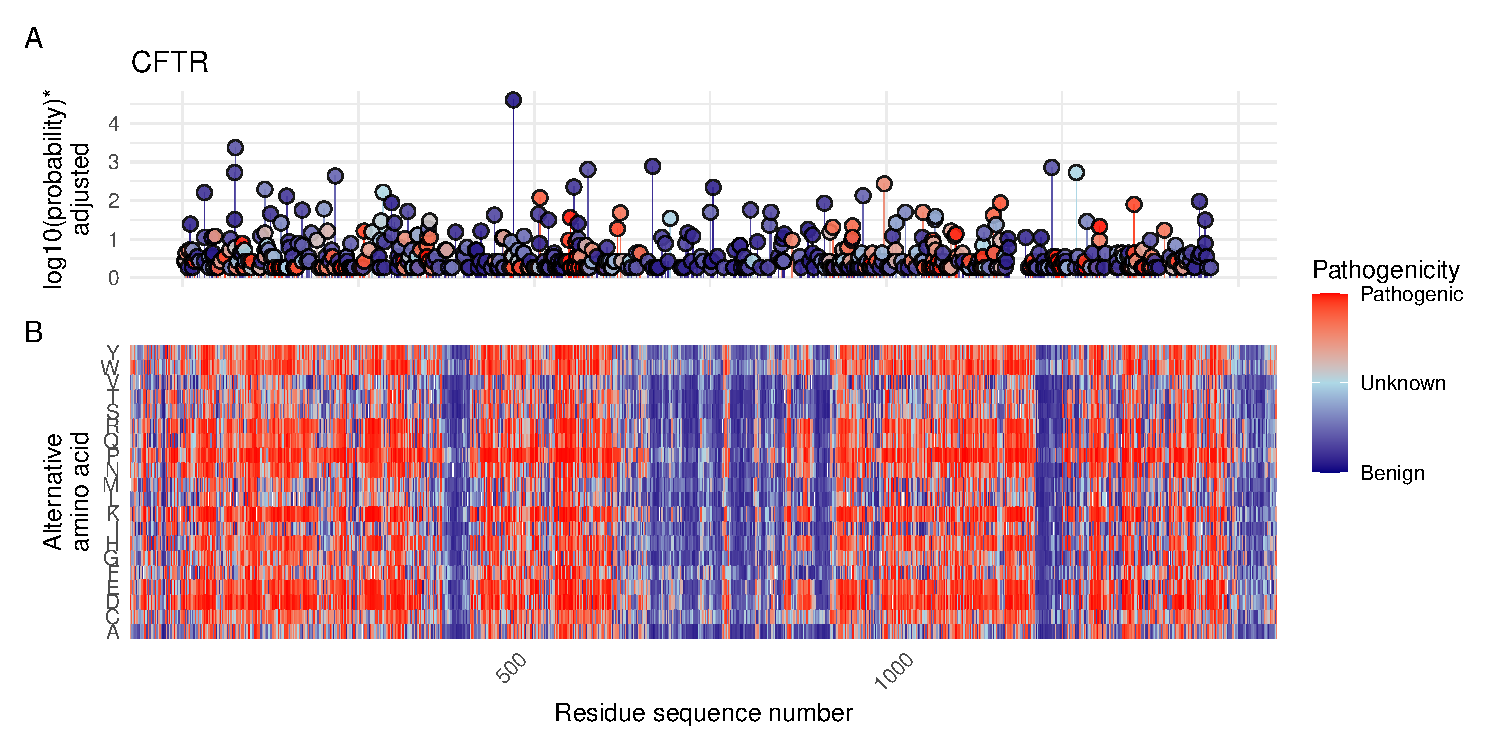
\includegraphics[width=0.8\textwidth]{../images/p_alphamissense_CFTR.pdf}
\end{center}
\caption{\textbf{(A) Probabilities of observing a patient with (B) AlphaMissense-derived pathogenicity scores.} Although AlphaMissense provides scores for every possible amino acid substitution, the most frequently observed variants in patients tend to be classified as benign or of unknown significance. This juxtaposition contextualises the likelihood of disease-associated substitutions and underlines prospects for refining predictive models. *Axis scaling for visibility near zero. Higher point indicates higher probability.}
 \label{fig:alphamissense}
\end{figure}

\FloatBarrier
\subsection{Integration of variant probabilities into IEI genetics data}
We integrated the computed prior probabilities for observing variants in all known genes associated with a given phenotype \cite{poli_human_2025}, across \ac{ad}, \ac{ar}, and \ac{xl} \ac{moi}, into our \ac{iei} genetics framework. These calculations, derived from gene panels in PanelAppRex, have yielded novel insights for the \ac{iei} disease panel. The final result comprised of machine- and human-readable datasets, including the table of variant classifications and priors available via a the linked repository \cite{lawless_2025_15111584}, and a user-friendly web interface that incorporates these new metrics.

\textbf{Figure \ref{fig:var_risk_est_iei_genetics}} shows the interface summarising integrated variant data. 
We include pre-calculated summary statistics and clinical significance as numerical metrics. 
Key quantiles (min, Q1, median, Q3, max) for each gene are rendered as sparkline box plots, and dynamic URLs link table entries to external databases (e.g. ClinVar, \ac{omim}, AlphaFold) 
as per \textbf{Section \ref{sec:pro_obs}}.
The prepared data are available for bioinformatic application 
\cite{lawless_2025_15111584} 
as per \textbf{Section \ref{sec:intregrate_tp_fn}}.


\begin{figure}[ht]
  \centering
  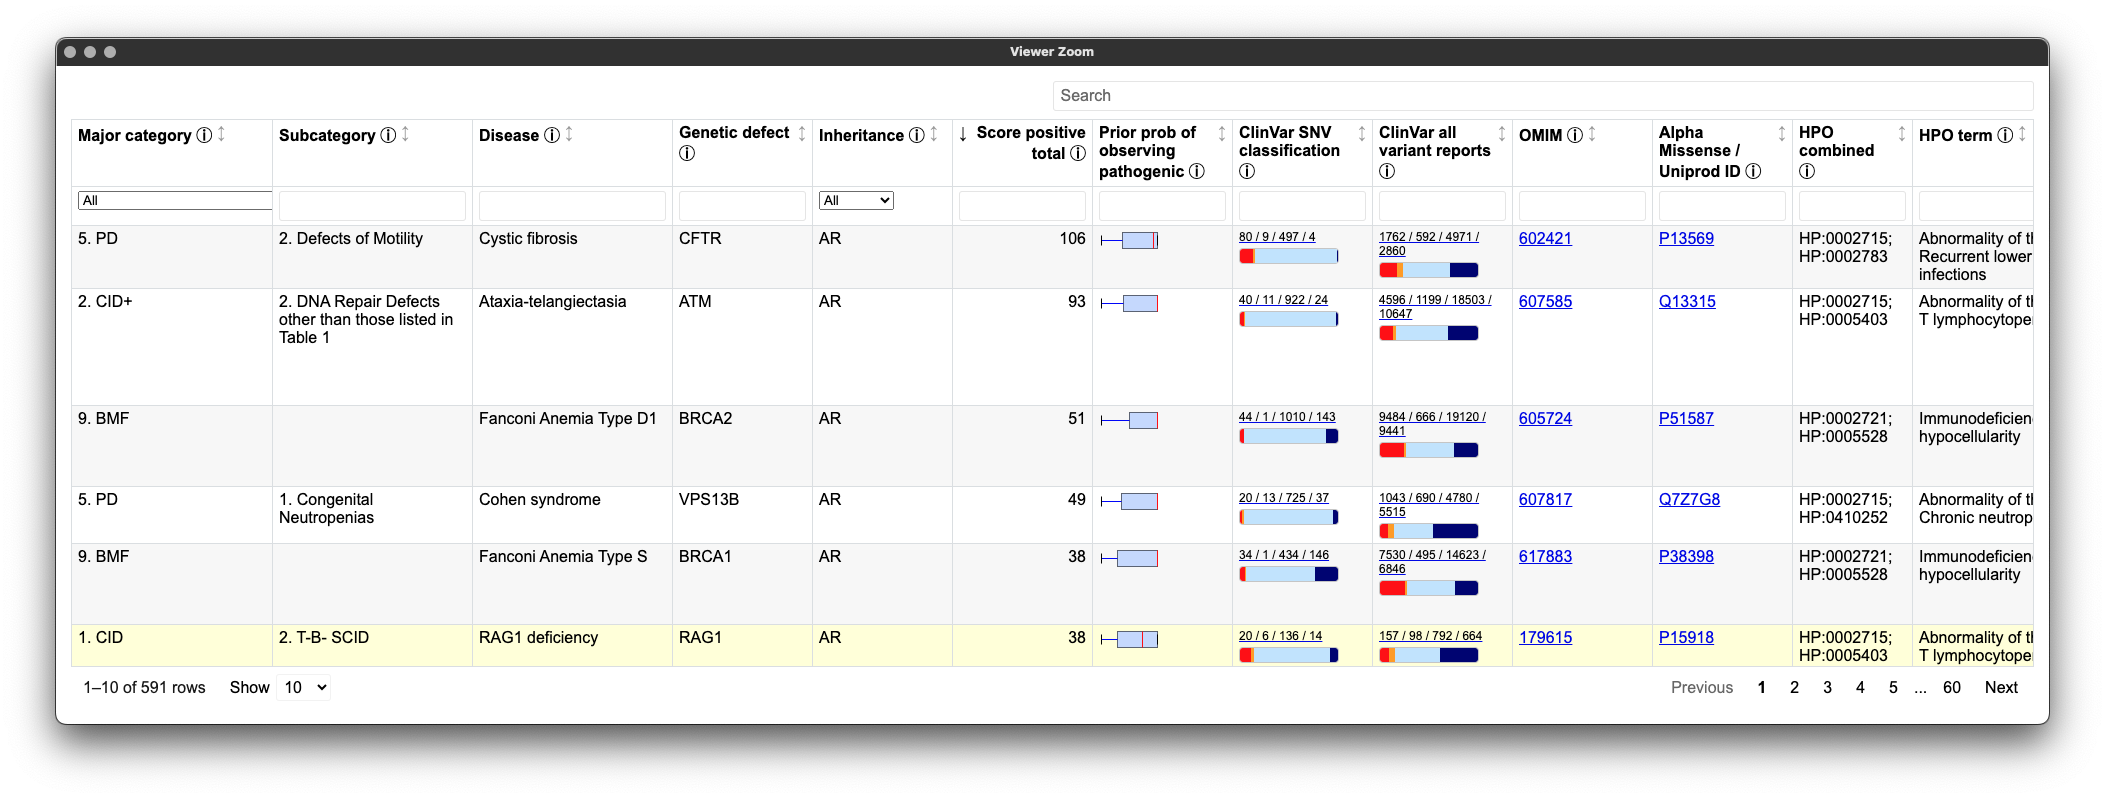
\includegraphics[width=1\textwidth]{../images/var_risk_est_iei_genetics.png}
  \caption{
    \textbf{Integration of variant probabilities into the \ac{iei} genetics framework.}
    The interface summarises the condensed variant data, with pre-calculated summary statistics and dynamic links to external databases. This integration enables immediate access to detailed variant classifications and prior probabilities for each gene.
  }
  \label{fig:var_risk_est_iei_genetics}
\end{figure}

\FloatBarrier
\clearpage
\section{Discussion}

% 1. Occurrence probability across disease genes
Our study presents, to our knowledge, the first comprehensive framework for calculating prior probabilities of observing disease-associated variants and the first to demonstrate the method for an evidence-aware genetic diagnosis with \ac{cri} \cite{hannah_using_2024, bick_estimating_2025}.
By integrating large-scale genomic annotations, including population allele frequencies from \ac{gnomad} \cite{karczewski2020mutational}, variant classifications from ClinVar \cite{landrum_clinvar_2018}, and functional annotations from resources such as \ac{dbnsfp}, with classical \ac{hwe}-based calculations, we derived robust estimates for 54,814 ClinVar variant classifications across 557 \ac{iei} genes implicated in \ac{pid} and monogenic inflammatory bowel disease \cite{lawless_panelapprex_2025, poli_human_2025}.
Although our results focus on \ac{iei}, the genome-wide framework also supports all inheritance patterns: \ac{ad} and \ac{xl} require a single pathogenic allele, whereas \ac{ar} demands homozygous or compound heterozygous states. Classical \ac{hwe}-based estimates thus furnish baseline occurrence probabilities and serve as robust priors for Bayesian risk models, a practice underutilised until the advent of large-scale databases \cite{landrum_clinvar_2018, karczewski2020mutational, lawless_panelapprex_2025, cheng_accurate_2023}. 

% 2. Integrating observed true positives and unobserved false negatives into a single actionable conclusion
A major deficit in current clinical genetics is the prevailing focus on confirming only the presence of \ac{tp} variants.
Our approach yielded three key results to overcome this hurdle. 
We generated per-variant priors across all \ac{moi}. 
The patient's results of observed and unobserved variants were integrated into a single posterior probability of carrying a damaging causal allele. 
As demonstrated in 
\textbf{Table \ref{tab:table_scenario_2_quant_uncert_ci}} and
\textbf{Figure \ref{fig:plot_scenario_2_quant_uncert_ci}}, 
this key result delivers a clinically applicable, interpretable probability that combines both detected and potentially unobserved variants.
% Score-positive-total decision aid
When whole-genome sequencing analyses are not yet available, the score-positive-total metric can serve as an optional decision aid, enabling manual, evidence-based ranking of candidate genes to prioritise diagnoses in patients with overlapping phenotypes.

% 0. Deficiencies
We acknowledge that our framework is currently focused (but not restricted) on \ac{snv}s and does not incorporate numerous other complexities of genetic disease, such as structural variants, de novo variants, hypomorphic alleles, overdominance, variable penetrance, tissue-specific expression, the Wahlund effect, pleiotropy, and others \cite{zschocke_mendelian_2023}. 
In certain applications, more refined estimates would benefit from including factors such as embryonic lethality, condition-specific penetrance, and age of onset \cite{hannah_using_2024}. 
Our analysis also relies on simplifying assumptions of random mating, an effectively infinite population, and the absence of migration, novel mutations, or natural selection.
% 8. Genome-wide gene distribution and linkage disequilibrium
We demonstrated the genome-wide gene distribution and \ac{moi} for the \ac{iei} panel relative to \ac{ld} showing that it is an important consideration and is feasible.
However, \ac{ld} is a challenging feature that requires accurate implementation which depends on the whole genome population-based pairwise genotype matrices for the given population. 
We used the reference global population \ac{af}s, which is more generalisable but less accurate than population-specific \ac{af} values.

% 3. Scenario one – simple diagnosis
% 4. Scenario two – complex diagnosis
% 5. Scenario three – currently impossible diagnosis
In the example single-case diagnosis scenarios, our approach enabled high-confidence attribution to a known pathogenic variant while also capturing the potential impact of a likely-pathogenic splice-site allele that was missed by sequencing. Scenario two showed a common diagnostic challenge where a strong candidate exists alongside an unconfirmed but plausible alternative. Our method distributes confidence across both possibilities. Conventional approaches focus only on detecting \ac{tp} and cannot provide this insight. By quantifying residual uncertainty, we can generate structured reports that clearly distinguish supported, excluded, and plausible-but-unseen variants. We call this ``evidence-aware'' interpretation.
When combined with genome-wide priors from the full range of disease-gene panels, this approach applies to any phenotype from PanelAppRex. By combining variant classification, allele frequency, \ac{moi}, and sequencing quality metrics, our method creates a scalable foundation for evidence-aware diagnostics in clinical genomics.

% Probability model
Estimating disease risk in genetic studies is complicated by uncertainties in key parameters such as variant penetrance and the fraction of cases attributable to specific variants \cite{zschocke_mendelian_2023}. 
In the simplest model, where a single, fully penetrant variant causes disease, the lifetime risk \(P(D)\) is equivalent to the genotype frequency \(P(G)\). 
For an allele with frequency \(p\) (ignoring \ac{ld} for \ac{ar}), this translates to:

\[
\begin{aligned}
\text{Autosomal Recessive:} \quad P(D) &= p^2, \\
\text{Autosomal Dominant:} \quad P(D) &= 2p(1-p) \approx 2p.
\end{aligned}
\]

When penetrance is incomplete, defined as \(P(D\mid G)\), the risk becomes:
$P(D) = P(G)\,P(D\mid G).$
In more realistic scenarios where multiple variants contribute to disease, \(P(G\mid D)\) denotes the fraction of cases attributable to a given variant. This leads to:

\[
P(D) = \frac{P(G)\,P(D\mid G)}{P(G\mid D)}.
\]
% 6. Validation studies
Because both penetrance and \(P(G\mid D)\) are often uncertain, solving this equation systematically poses a major challenge, which we incidentally tackled in the validation studies
\cite{minikel_quantifying_2016, whiffin_using_2017}. % Eric's \url{https://www.cureffi.org/2019/06/05/using-genetic-data-to-estimate-disease-prevalence/}.

Our framework addresses this challenge by combining variant classifications, population allele frequencies, and curated gene-disease associations. 
While imperfect on an individual level, these sources exhibit predictable aggregate behaviour, supported by James-Stein estimation principles \cite{efron_steins_1973}.
% Keep this thought here: Stein's Estimation Rule and its competitors, as discussed by Efron and Morris (1973), demonstrate that shrinkage estimators—such as the James–Stein estimator—can outperform traditional maximum likelihood methods by “borrowing strength” across multiple parameters. In essence, even if individual estimates are noisy or imprecise, shrinking them towards a common value (or mean) improves the overall risk (mean squared error) of the estimates. This empirical Bayes approach shows that aggregate estimates tend to be well-calibrated, a principle we leverage in our work: although individual ClinVar variant classifications may be uncertain, their collective behaviour yields robust and reliable prior probabilities when combined with population allele frequencies and curated gene–disease associations.
Curated gene-disease associations help identify genes that are explainable for most disease cases, allowing us to approximate \(P(G\mid D)\) close to one. In this way, we obtain robust estimates of \(P(G)\) (the frequency of disease-associated genotypes), even when exact values of penetrance and case attribution remain uncertain.

This approach allows us to pre-calculate priors and summarise the overall pathogenic burden.
By focusing on a subset \(\mathcal{V}\) of variants that pass stringent filtering, where each \(P(G_i \mid D)\) is the probability that a case of disease \(D\) is attributable to variant(s) \(i\), we assume that, in aggregate,

\[
\sum_{i\in\mathcal{V}} P(G_i\mid D) \approx 1.
\]

Even if the cumulative contribution is slightly less than one, the resultant risk estimates remain robust within the broad \ac{cri}s typical of epidemiological studies. 
By incorporating these pre-calculated priors into a Bayesian framework, our method refines risk estimates and enhances clinical decision-making despite inherent uncertainties.

% 9. Novel PID classifications from genetic PPI and clinical features
% 11. Integration of variant probabilities into the IEI genetics framework
% 7. Genetic constraint in high-impact protein networks
% Our results refine risk calculations by incorporating \ac{moi} complexities and enhances clinicians’ understanding of expected variant occurrences, thereby improving diagnostic precision.
For the \ac{iei}-specific investigation, 
we showed that immunophenotypic and network-derived features can be used to train and test models that predict \ac{ppi}s. From this, we derived a new, simplified classification of immune features for \ac{iei} genes. We have listed the new immunophenotypic categories (e.g. T cell low)  in the user database, however we have not included the detailed cluster assignments (e.g. \ac{ppi} groups) because they are too complex for direct interpretation manually. Instead, our demonstration provides worked examples that bioinformaticians can use to perform more refined clustering in larger studies.

Moreover, because variant sets can be collapsed instead of relying on the gene-level, our method complements existing statistical approaches for aggregating variant effects with methods like \ac{skat} and \ac{acat} \cite{liu2019acat,li2020dynamic,wu2011rare,lee2012optimal} and multi-omics integration techniques \cite{kong2018nature,howe2021within}.
It also remains consistent with established variant interpretation guidelines from the \ac{acmg} \cite{richards2015standards} and complementary frameworks \cite{tavtigian2020fitting,li2017intervar}, as well as \ac{qc} protocols \cite{pedersen2021effective,anderson2010data}. 
Standardised reporting for qualifying variant sets, such as \ac{acmg} Secondary Findings v3.2 \cite{miller2023acmg}, further contextualises the integration of these probabilities into clinical decision-making.

% 10. Probability of observing AlphaMissense pathogenicity
We compared our occurrence probabilities with AlphaMissense pathogenicity scores and observed that common variants are predominantly scored as benign or of uncertain significance. While this aligns with their allele frequencies, any pathogenic variant seen in a patient warrants evaluation against its prior observation probability to assess causality. Predictive tools such as AlphaMissense could ostensibly enhance their embedding of variant features by incorporating gene-disease associations and \ac{moi} data, which may not be fully represented by raw population allele frequencies.

Future work should incorporate the additional variant types and models to further refine these probability estimates. 
By continuously updating classical estimates with emerging data and prior knowledge, we aim to enhance the precision of genetic diagnostics and ultimately improve patient care.

\clearpage
\section{Conclusion}
Our work generates prior probabilities for observing any variant classification in \ac{iei} genetic disease, providing a quantitative resource to enhance Bayesian variant interpretation and clinical decision-making.

\section*{Acknowledgements}
\noindent
We would like to thank all the patients and families who have been providing advice on SwissPedHealth and its projects, as well as the clinical and research teams at the participating institutions.
We acknowledge Genomics England for providing public access to the PanelApp data.
The use of data from Genomics England panelapp was licensed under the Apache License 2.0.
The use of data from \ac{uniprot} was licensed under Creative Commons Attribution 4.0 International (CC BY 4.0).
ClinVar asks its users who distribute or copy data to provide attribution to them as a data source in publications and websites \cite{landrum_clinvar_2018}.
\ac{dbnsfp} version 4.4a is licensed under the Creative Commons Attribution-NonCommercial-NoDerivatives 4.0 International (CC BY-NC-ND 4.0); while we cite this dataset as used our research publication, it is not used for the final version which instead used ClinVar and \ac{gnomad} directly.
GnomAD is licensed under  Creative Commons  Zero Public Domain Dedication (CC0 1.0 Universal).
GnomAD request that usages cites the \ac{gnomad} flagship paper \cite{karczewski2020mutational}
and any online resources that include the data set provide a link to the browser, and note that tool includes data from the \ac{gnomad} v4.1 release.
AlphaMissense asks to cite \citet{cheng_accurate_2023} for usage in research, with data available from \citet{jun_cheng_2023_8208688}.


\section*{Contributions}
\noindent 
DL performed main analyses and wrote the manuscript.
SB, AS, MS, and JT designed analysis and wrote the manuscript.
JF, LJS supervised the work, and applied for funding.
The Quant Group is a collaboration across multiple institutions where authors contribute equally; the members on this project were DL, SB, AS, and MS.

\section*{Competing interest}
\noindent
The authors declare no competing interest. 

\section*{Ethics statement}
\noindent
This study only used data which was previously published and publicly available, as cited in the manuscript.
This  SwissPedHealth study, under which this work was carried out, was approved based on the advice of the ethical committee Northwest and Central Switzerland (EKNZ, AO\_2022-00018). 
The study was conducted in accordance with the Declaration of Helsinki.

\section*{Funding}
\noindent This project was supported through the grant Swiss National Science Foundation (SNF) 320030\_201060, and NDS-2021-911 (SwissPedHealth) from the Swiss Personalized Health Network and the Strategic Focal Area `Personalized Health and Related Technologies' of the ETH Domain (Swiss Federal Institutes of Technology).

% \newpage
\bibliographystyle{unsrtnat}
\bibliography{references}

\clearpage
%\\\\\\\\\\\\\\\\\\\\\\\\\\\\
\beginsupplement
\section{Supplemental} \label{Supplemental_text}

Supplemental data are presented under the same headings that correspond to their relevant main text sections. 

\subsection{Variant class occurrence probability}
\begin{figure}[ht]
  \centering
  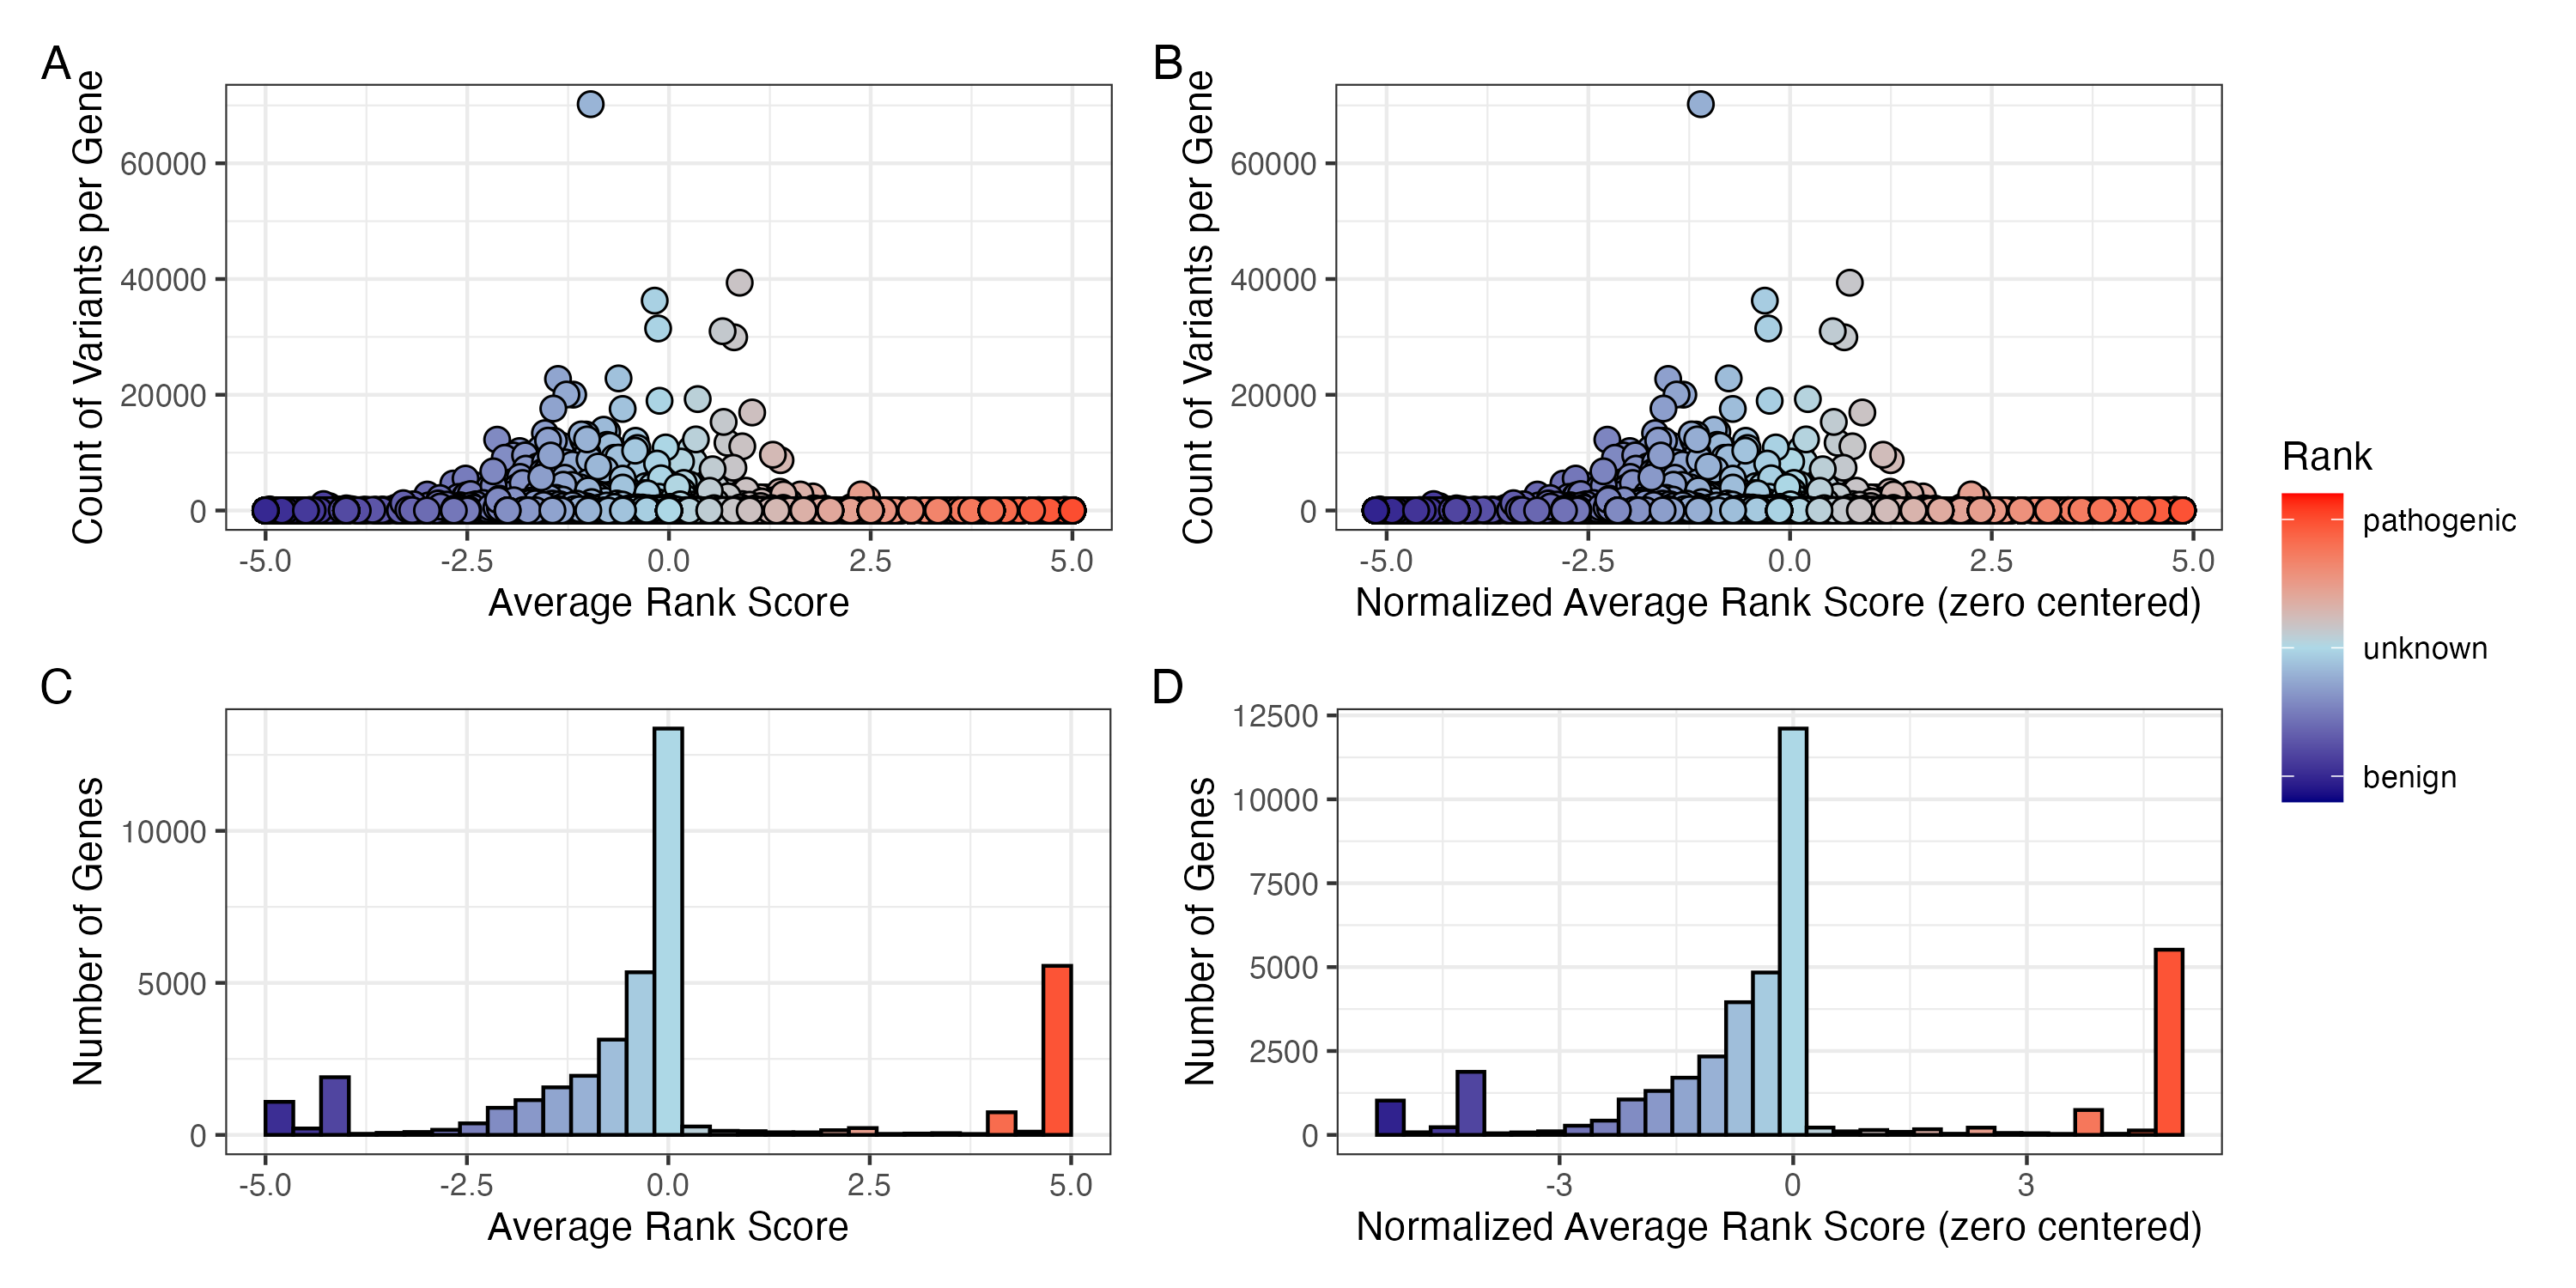
\includegraphics[width=0.99\textwidth]{../images/p_gene_summary_hist_patch3.png}
\caption{\textbf{Global distribution of ClinVar clinical-significance classification scoring.} 
(A) Number of variants per gene containing the assigned score for each ClinVar classification term (−5 to +5). 
(B) The same data after normalisation by zero centring the average rank score.
(C) The tally of genes for their average rank and (D) after normalisation. No normalisation was required for the scoring system as shown by comparison of A-C and B-D.}
  \label{fig:p_gene_summary_hist_patch3}
\end{figure}

\clearpage
\subsection{Integrating observed true positives and unobserved false negatives into a single, actionable conclusion}

\begin{table}[!h]
\centering
\caption{Result of clinical genetics diagnosis scenario 1 including metadata. The most strongly supported observed variant was \texttt{p.Ser237Ter} (posterior: 0.594). The strongest unsequenced variant was \texttt{p.Thr567Ile} (posterior: 0). The total probability of a causal diagnosis given the available evidence was 1 (95\% CI: 1--1).\label{tab:table_scenario_1_quant_uncert_ci}}
\centering
\resizebox{\ifdim\width>\linewidth\linewidth\else\width\fi}{!}{
\begin{tabular}[t]{>{\raggedright\arraybackslash}p{2.5cm}>{\raggedright\arraybackslash}p{1.5cm}>{\raggedright\arraybackslash}p{1.5cm}>{\raggedleft\arraybackslash}p{1.5cm}>{\raggedleft\arraybackslash}p{1.8cm}>{\raggedleft\arraybackslash}p{1.5cm}>{\raggedleft\arraybackslash}p{1.5cm}>{\raggedleft\arraybackslash}p{1.5cm}>{\raggedleft\arraybackslash}p{1.5cm}>{\raggedleft\arraybackslash}p{1.5cm}>{\raggedleft\arraybackslash}p{1.5cm}>{\raggedleft\arraybackslash}p{1.5cm}>{\raggedleft\arraybackslash}p{1.5cm}}
\toprule
Variant & Flag & Class & Evidence Score & Occurrence Prob & Adj Occ Prob & Alpha & Beta & Lower & Median & Upper & Posterior Share & Prob Causal\\
\midrule
p.Ser237Ter & present & causal & 5 & 0.000 & 0 & 6 & 371 & 0.004 & 0.142 & 0.803 & 0.594 & 0.594\\
p.Thr567Ile & missing & other & -5 & 0.002 & 0 & 1 & 363 & NA & NA & NA & 0.000 & 0.000\\
p.Arg231His & present & other & 0 & 0.000 & 0 & 1 & 361 & 0.004 & 0.142 & 0.803 & 0.000 & 0.000\\
p.Gly650Arg & present & other & 0 & 0.000 & 0 & 1 & 379 & 0.004 & 0.142 & 0.803 & 0.000 & 0.000\\
p.Val236Ile & missing & other & 0 & 0.000 & 0 & 1 & 351 & NA & NA & NA & 0.000 & 0.000\\
\addlinespace\\
Total & NA & NA & NA & NA & NA & NA & NA & 1.000 & 1.000 & 1.000 & NA & 1.000\\
\bottomrule
\end{tabular}}
\end{table}


\begin{table}[!h]
\centering
\caption{Result of clinical genetics diagnosis scenario 2. The most strongly supported observed variant was \texttt{p.Ser237Ter} (posterior: 0.399). The strongest unsequenced variant was \texttt{c.159+1G>A} (posterior: 0.339). The total probability of a causal diagnosis given the available evidence was 0.542 (95\% CI: 0.264--0.8).\label{tab:table_scenario_2_quant_uncert_ci}}
\centering
\resizebox{\ifdim\width>\linewidth\linewidth\else\width\fi}{!}{
\begin{tabular}[t]{>{\raggedright\arraybackslash}p{2.5cm}>{\raggedright\arraybackslash}p{1.5cm}>{\raggedright\arraybackslash}p{1.5cm}>{\raggedleft\arraybackslash}p{1.5cm}>{\raggedleft\arraybackslash}p{1.8cm}>{\raggedleft\arraybackslash}p{1.5cm}>{\raggedleft\arraybackslash}p{1.5cm}>{\raggedleft\arraybackslash}p{1.5cm}>{\raggedleft\arraybackslash}p{1.5cm}>{\raggedleft\arraybackslash}p{1.5cm}>{\raggedleft\arraybackslash}p{1.5cm}>{\raggedleft\arraybackslash}p{1.5cm}>{\raggedleft\arraybackslash}p{1.5cm}}
\toprule
Variant & Flag & Class & Evidence Score & Occurrence Prob & Adj Occ Prob & Alpha & Beta & Lower & Median & Upper & Posterior Share & Prob Causal\\
\midrule
p.Ser237Ter & present & causal & 5.0 & 0.000 & 0 & 6.0 & 345 & 0.003 & 0.092 & 0.576 & 0.399 & 0.399\\
c.159+1G>A & missing & causal & 4.5 & 0.000 & 0 & 5.5 & 373 & NA & NA & NA & 0.339 & 0.339\\
p.Thr567Ile & missing & other & -5.0 & 0.002 & 0 & 1.0 & 353 & NA & NA & NA & 0.000 & 0.000\\
p.Arg231His & present & other & 0.0 & 0.000 & 0 & 1.0 & 347 & 0.003 & 0.092 & 0.576 & 0.000 & 0.000\\
p.Gly650Arg & present & other & 0.0 & 0.000 & 0 & 1.0 & 359 & 0.003 & 0.092 & 0.576 & 0.000 & 0.000\\
p.Val236Ile & missing & other & 0.0 & 0.000 & 0 & 1.0 & 361 & NA & NA & NA & 0.000 & 0.000\\
\addlinespace\\
Total & NA & NA & NA & NA & NA & NA & NA & 0.264 & 0.542 & 0.800 & NA & 0.542\\
\bottomrule
\end{tabular}}
\end{table}


\begin{table}[!h]
\centering
\caption{Result of clinical genetics diagnosis scenario 3 including metadata. No observed variants were detected in this scenario. The strongest unsequenced variant was \texttt{p.Cys243Arg} (posterior: 0.366). The total probability of a causal diagnosis given the available evidence was 0 (95\% CI: 0--0).\label{tab:table_scenario_3_quant_uncert_ci}}
\centering
\resizebox{\ifdim\width>\linewidth\linewidth\else\width\fi}{!}{
\begin{tabular}[t]{>{\raggedright\arraybackslash}p{2.5cm}>{\raggedright\arraybackslash}p{1.5cm}>{\raggedright\arraybackslash}p{1.5cm}>{\raggedleft\arraybackslash}p{1.5cm}>{\raggedleft\arraybackslash}p{1.8cm}>{\raggedleft\arraybackslash}p{1.5cm}>{\raggedleft\arraybackslash}p{1.5cm}>{\raggedleft\arraybackslash}p{1.5cm}>{\raggedleft\arraybackslash}p{1.5cm}>{\raggedleft\arraybackslash}p{1.5cm}>{\raggedleft\arraybackslash}p{1.5cm}>{\raggedleft\arraybackslash}p{1.5cm}>{\raggedleft\arraybackslash}p{1.5cm}}
\toprule
Variant & Flag & Class & Evidence Score & Occurrence Prob & Adj Occ Prob & Alpha & Beta & Lower & Median & Upper & Posterior Share & Prob Causal\\
\midrule
p.Cys243Arg & missing & causal & 5.0 & 0.000 & 0.000 & 6 & 341 & NA & NA & NA & 0.366 & 0.366\\
p.Tyr246Ter & missing & causal & 4.0 & 0.000 & 0.000 & 5 & 369 & NA & NA & NA & 0.284 & 0.284\\
p.Lys304Glu & missing & other & -5.0 & 0.000 & 0.000 & 1 & 353 & NA & NA & NA & 0.000 & 0.000\\
p.Ile207Leu & missing & other & -4.5 & 0.000 & 0.000 & 1 & 359 & NA & NA & NA & 0.000 & 0.000\\
p.His646Pro & missing & other & 0.0 & 0.002 & 0.001 & 1 & 377 & NA & NA & NA & 0.000 & 0.000\\
p.Arg280Trp & missing & other & -4.0 & 0.000 & 0.000 & 1 & 357 & NA & NA & NA & 0.000 & 0.000\\
p.Thr635Ile & missing & other & 0.0 & 0.000 & 0.000 & 1 & 349 & NA & NA & NA & 0.000 & 0.000\\
p.Arg162Trp & missing & other & 0.0 & 0.000 & 0.000 & 1 & 369 & NA & NA & NA & 0.000 & 0.000\\
\addlinespace\\
Total & NA & NA & NA & NA & NA & NA & NA & 0 & 0 & 0 & NA & 0.000\\
\bottomrule
\end{tabular}}
\end{table}


\begin{figure}[ht]
  \centering
  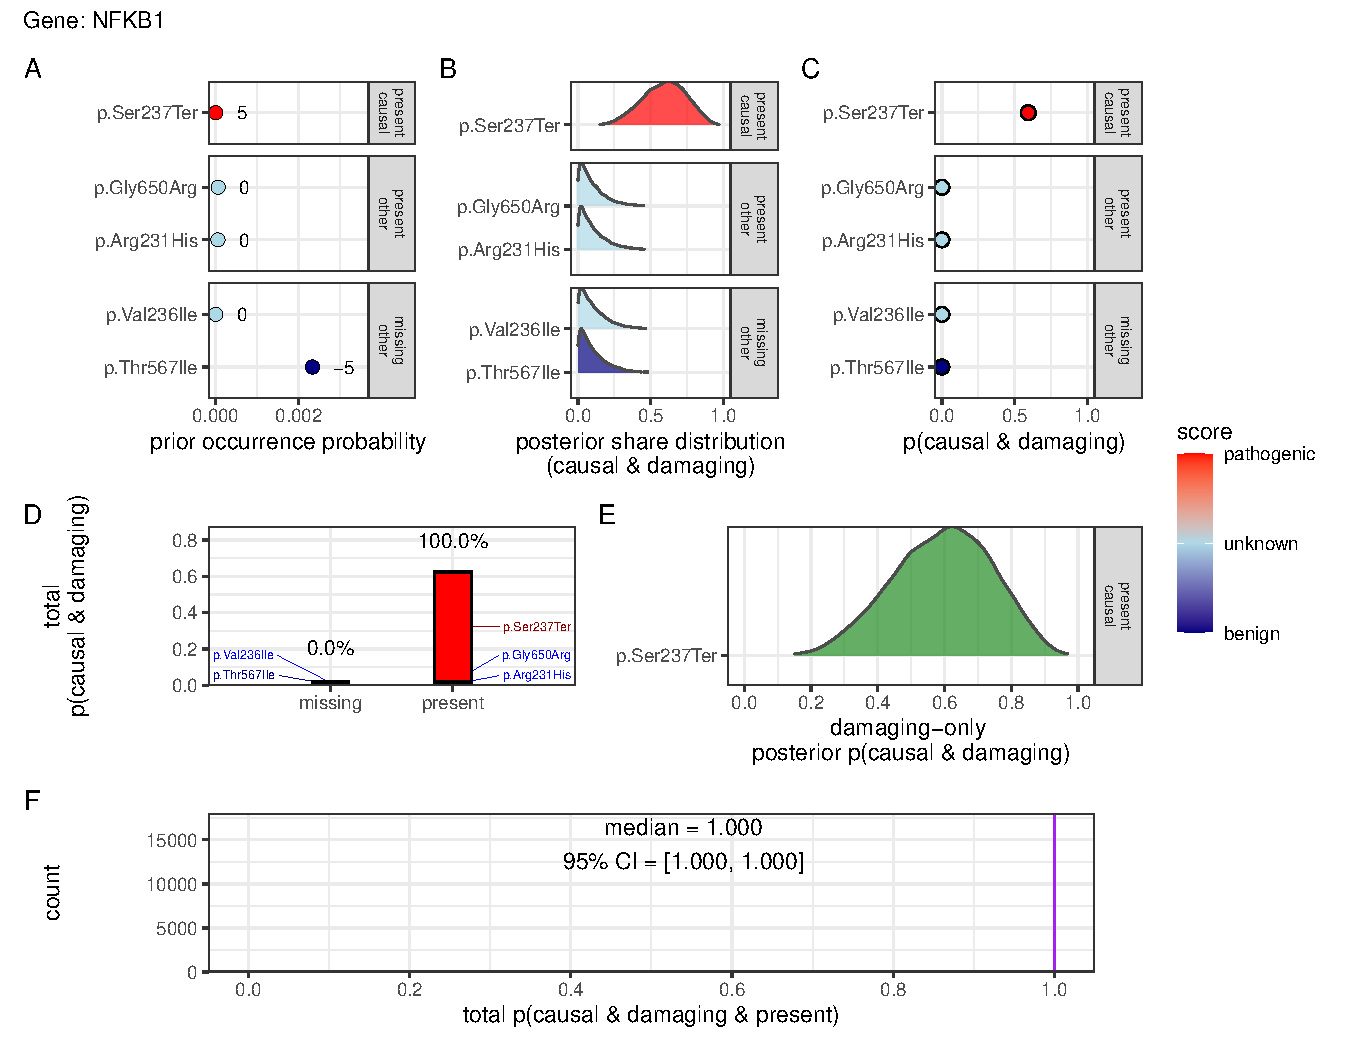
\includegraphics[width=0.99\textwidth]{../images/plot_scenario_1_quant_uncert_ci.pdf}
  \caption{
 \textbf{Quantification of present (\ac{tp}) and no missing (\ac{fn}) causal genetic variants for disease in \ac{nfkb1} (scenario 1)}.
  Only one known pathogenic variant, \texttt{p.Ser237Ter}, was observed and all previously reported pathogenic positions were successfully sequenced and confirmed as reference (true negatives).  
  Panels (A–F) follow the same structure as scenario 2 described in \textbf{Figure \ref{fig:plot_scenario_2_quant_uncert_ci}}, culminating in a gene-level posterior probability of 1 (95\,\% \ac{cri}: 0.99–1.00), with full support assigned to the observed allele given the available evidence. Pathogenicity scores (-5 to +5) are annotated.
  }
  \label{fig:plot_scenario_1_quant_uncert_ci}
\end{figure}

\begin{figure}[ht]
  \centering
  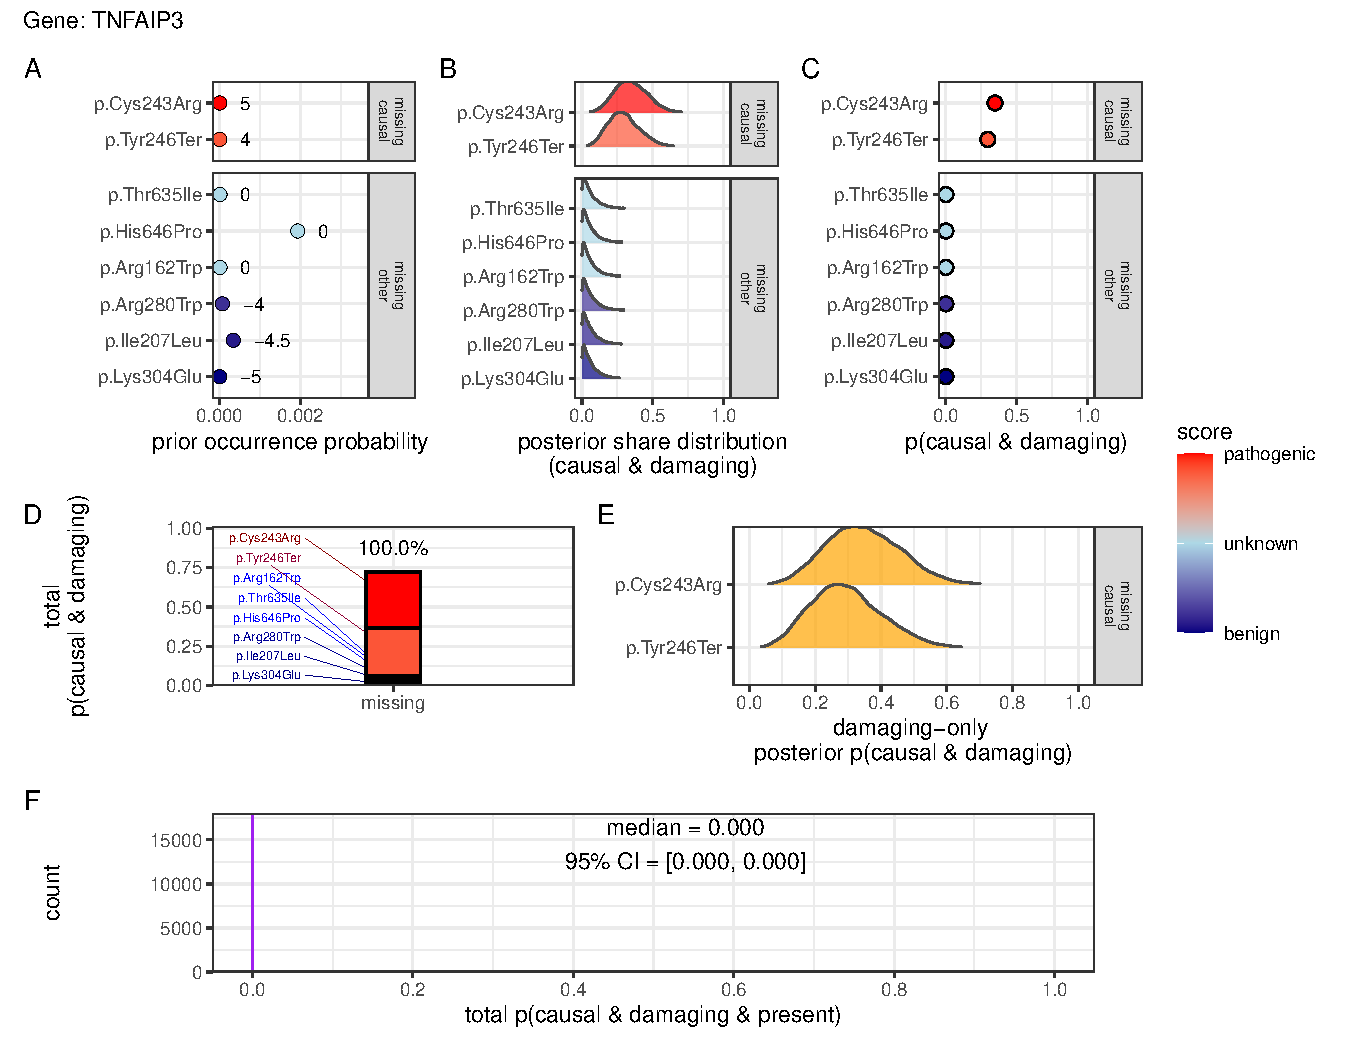
\includegraphics[width=0.99\textwidth]{../images/plot_scenario_3_quant_uncert_ci.pdf}
  \caption{
 \textbf{Quantification of no present (\ac{tp}) in \ac{nfkb1} and only missing (\ac{fn}) causal genetic variants for disease in \ac{tnfaip3} (scenario 3)}.
No known causal variants were observed in \ac{nfkb1}, but one representative unsequenced allele was selected from each distinct ClinVar classification and treated as a potential false negative.  
Panels (A–F) follow the same structure as scenario 2 described in \textbf{Figure \ref{fig:plot_scenario_2_quant_uncert_ci}}.  
The posterior reflects uncertainty across multiple plausible but unobserved variants, resulting in low \ac{cri} (0-0) and 100\% missing overall attribution in contrast to scenarios where known pathogenic variants were observed. For this patient, we have no evidence of a causal variant since the only top candidates are not yet accounted for.
Pathogenicity scores (-5 to +5) are annotated in (A).
  }
  \label{fig:plot_scenario_3_quant_uncert_ci}
\end{figure}

\FloatBarrier
\clearpage
\subsection{Validation studies}

\begin{figure}[ht]
  \centering
  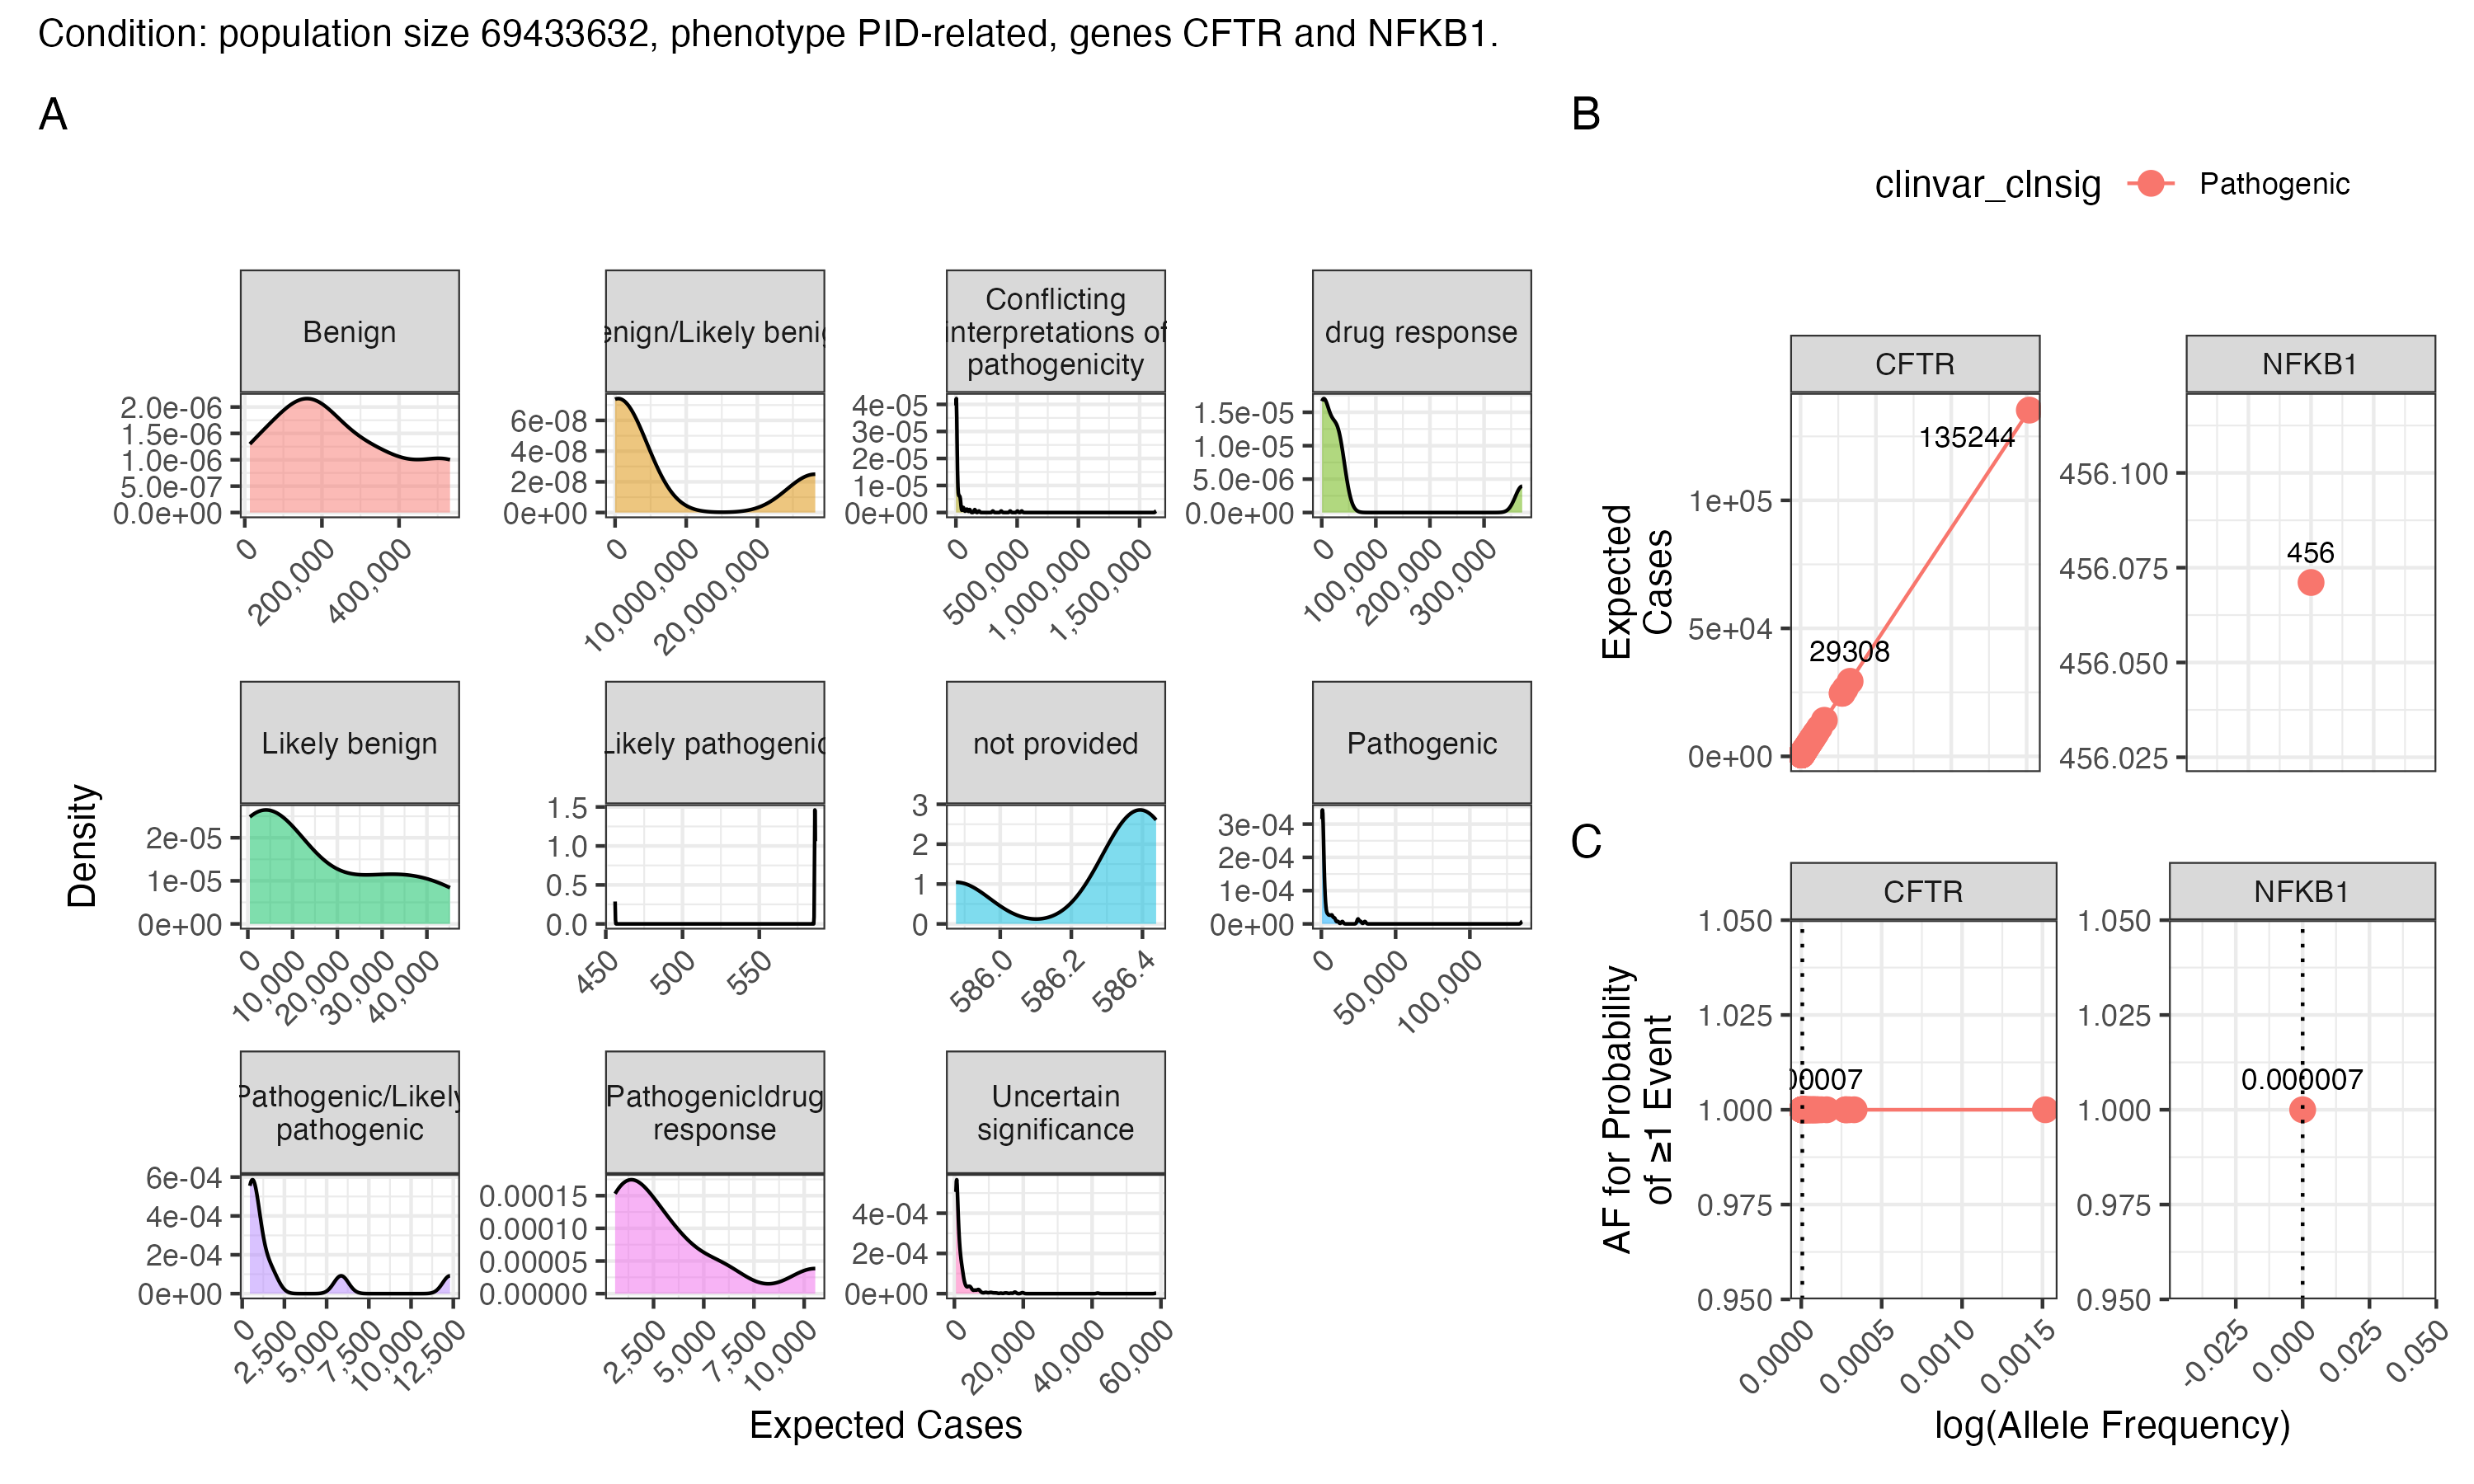
\includegraphics[width=\textwidth]{../images/validation_studies_scatterdense_expected_prob.png}
  \caption{\textbf{Interpretation of probability of observing a variant classification.} 
 The result from the chosen validation genes \ac{cftr} and \ac{nfkb1} are shown. 
 Case counts are dependant on the population size and phenotype.
(A) The density plots of expected observations by ClinVar clinical significance. 
We then highlight the values for pathogenic variants specifically showing;
(B) the allele frequency versus expected cases in this population size and
(C) the probability of observing at least one event in this population size.}
  \label{fig:validation_scatter_dense}
\end{figure}

\begin{figure}[ht]
  \centering
  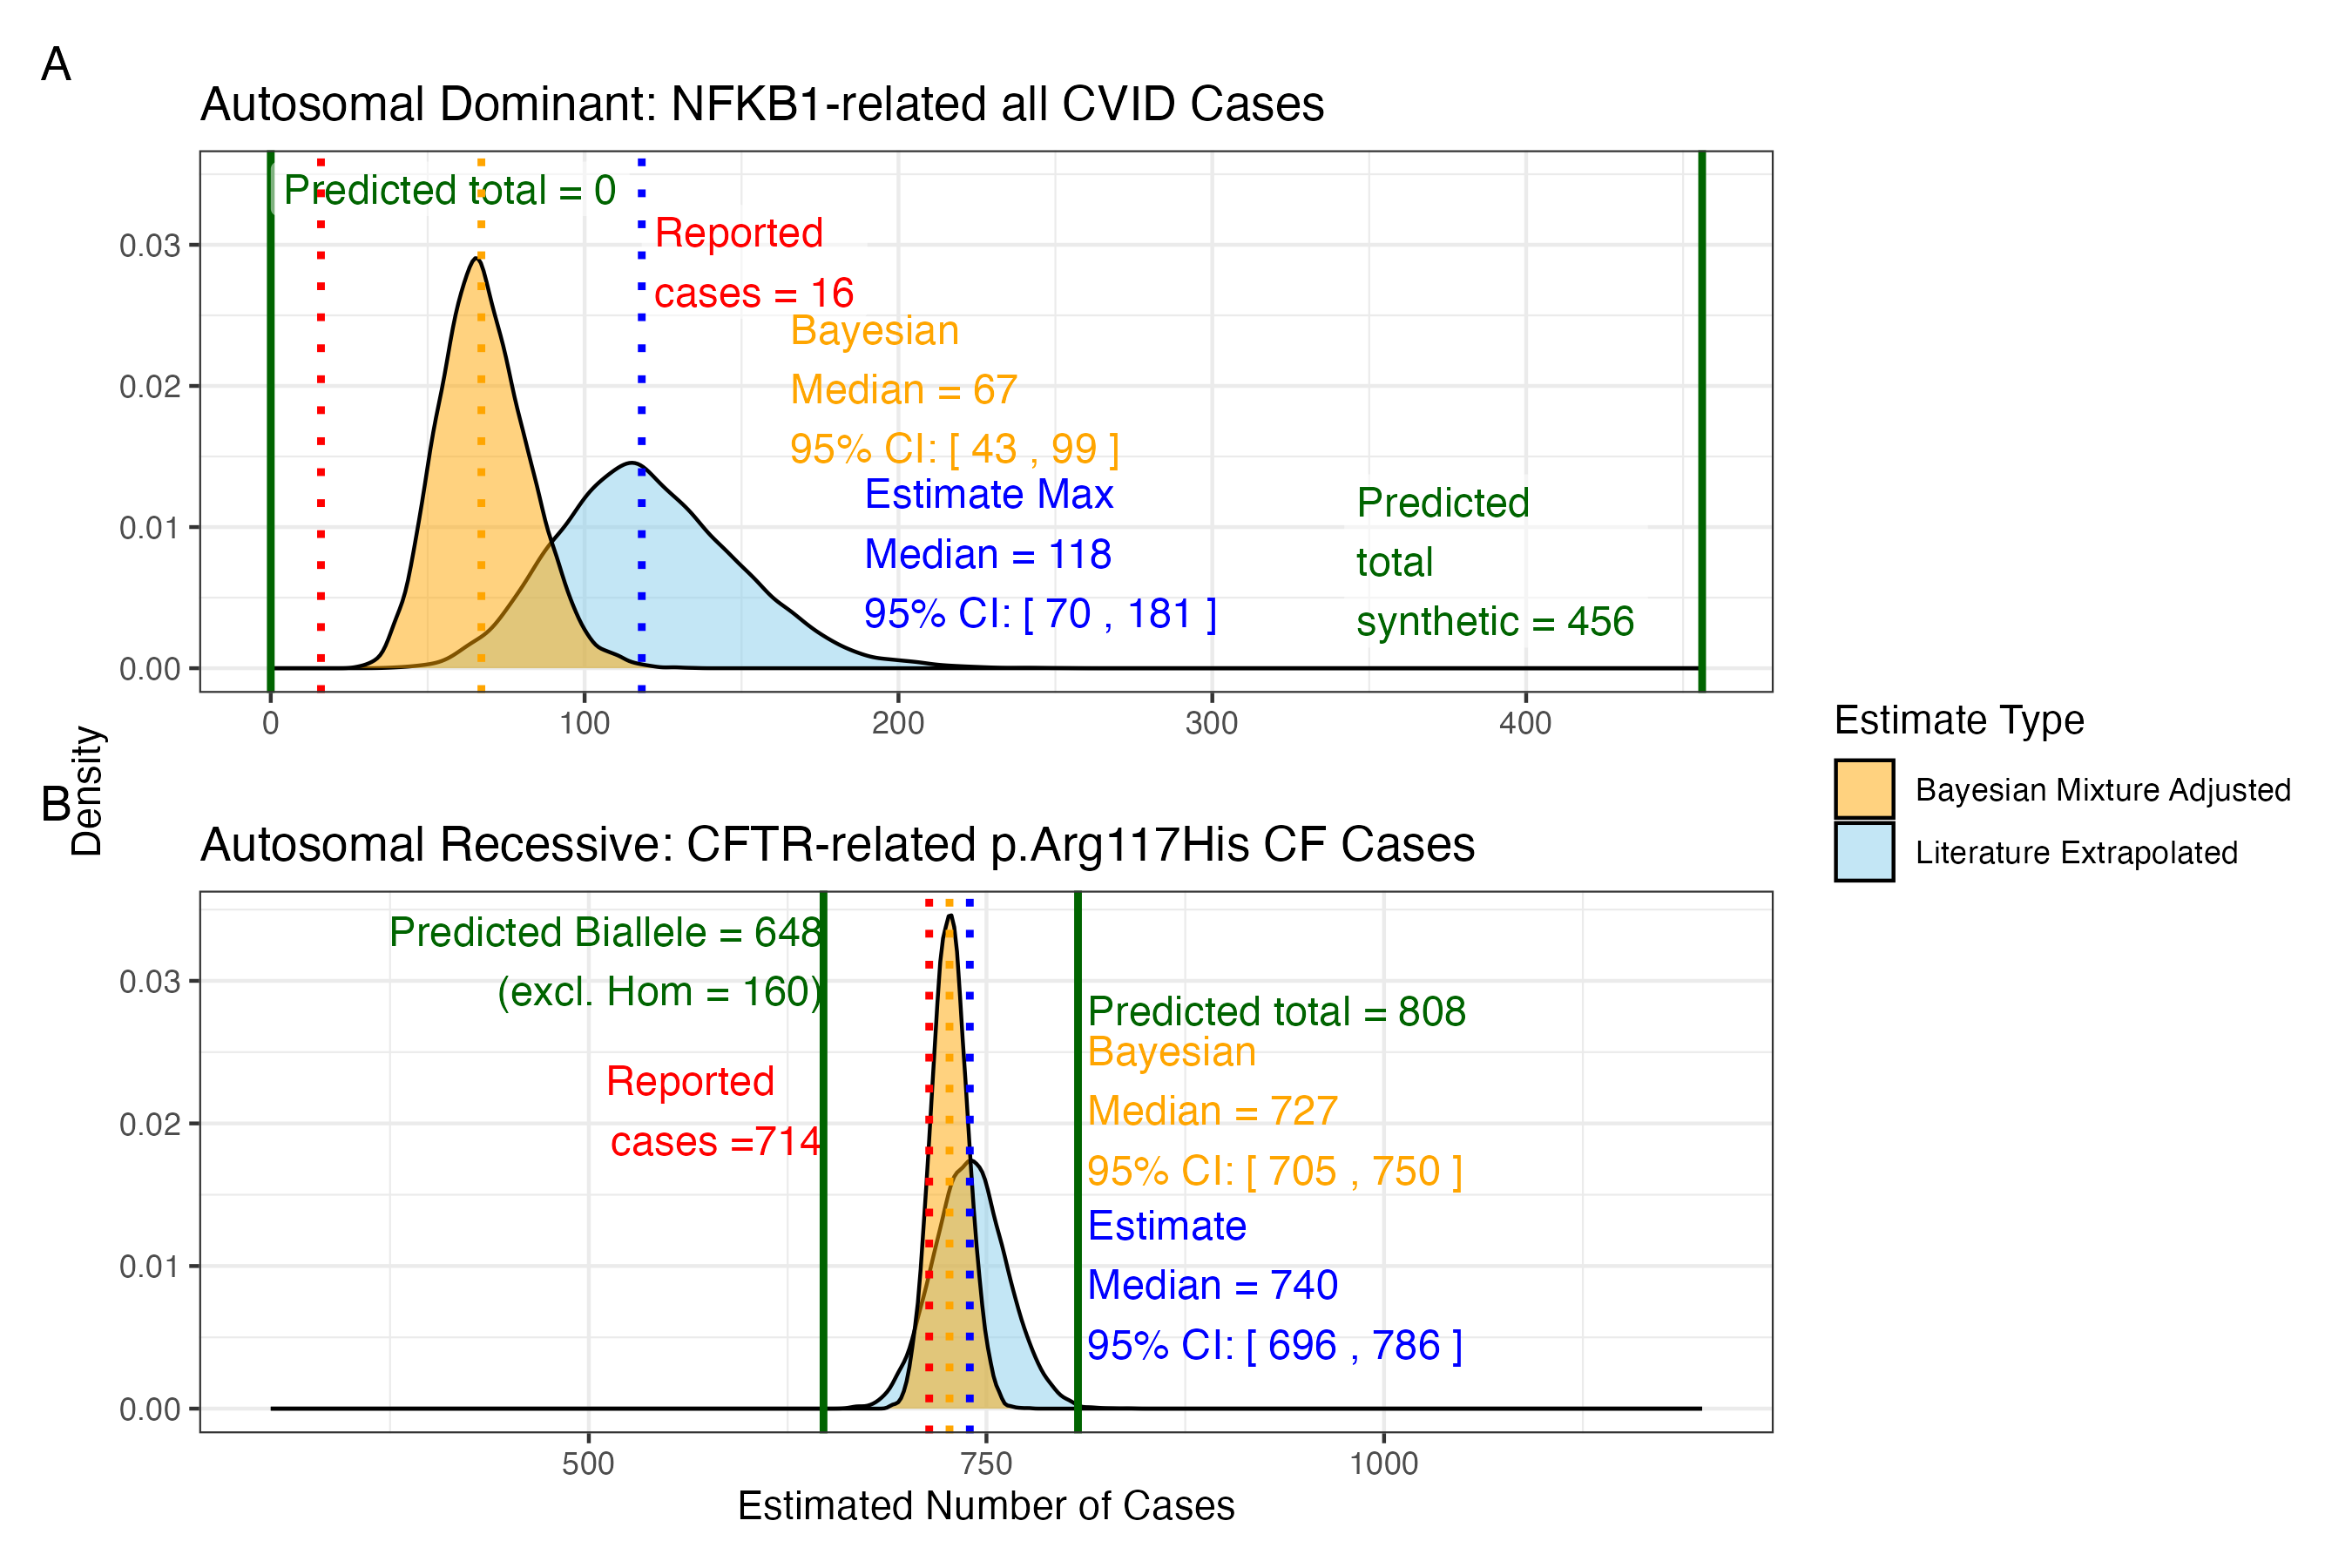
\includegraphics[width=0.99\textwidth]{../images/validation_studies_bayesian_adjusted_estimates.png}
  \caption{\textbf{Prior probabilities compared to validation disease cohort metrics.}
  (A) Density distributions for the number of \ac{nfkb1}-related \ac{cvid} cases in the UK. 
  Our model (green) predicted 456 cases, which falls between the observed cohort count (red) of 390 and the upper extrapolated values.
  The blue curve represents maximum count of 1280, and the orange curve shows the Bayesian-adjusted mixture estimate of 835. 
(B) Density distributions for \ac{cftr}-related \texttt{p.Arg117His} \ac{cf} cases. 
Our model (green) predicted 648 biallelic cases and 808 total cases.
The nationally reported case count (red) was 714.
The blue curve represents maximum extrapolated count of 740, and the orange curve shows the Bayesian-adjusted mixture estimate of 727. We observed close agreement among the reported disease cases and our integrated probability estimation framework.}
  \label{fig:validation_studies_bayesian_adjusted_estimates}
\end{figure}




\FloatBarrier
\clearpage
\subsubsection{Interpretation of ClinVar variant observations}

\begin{figure}[ht]
  \centering
  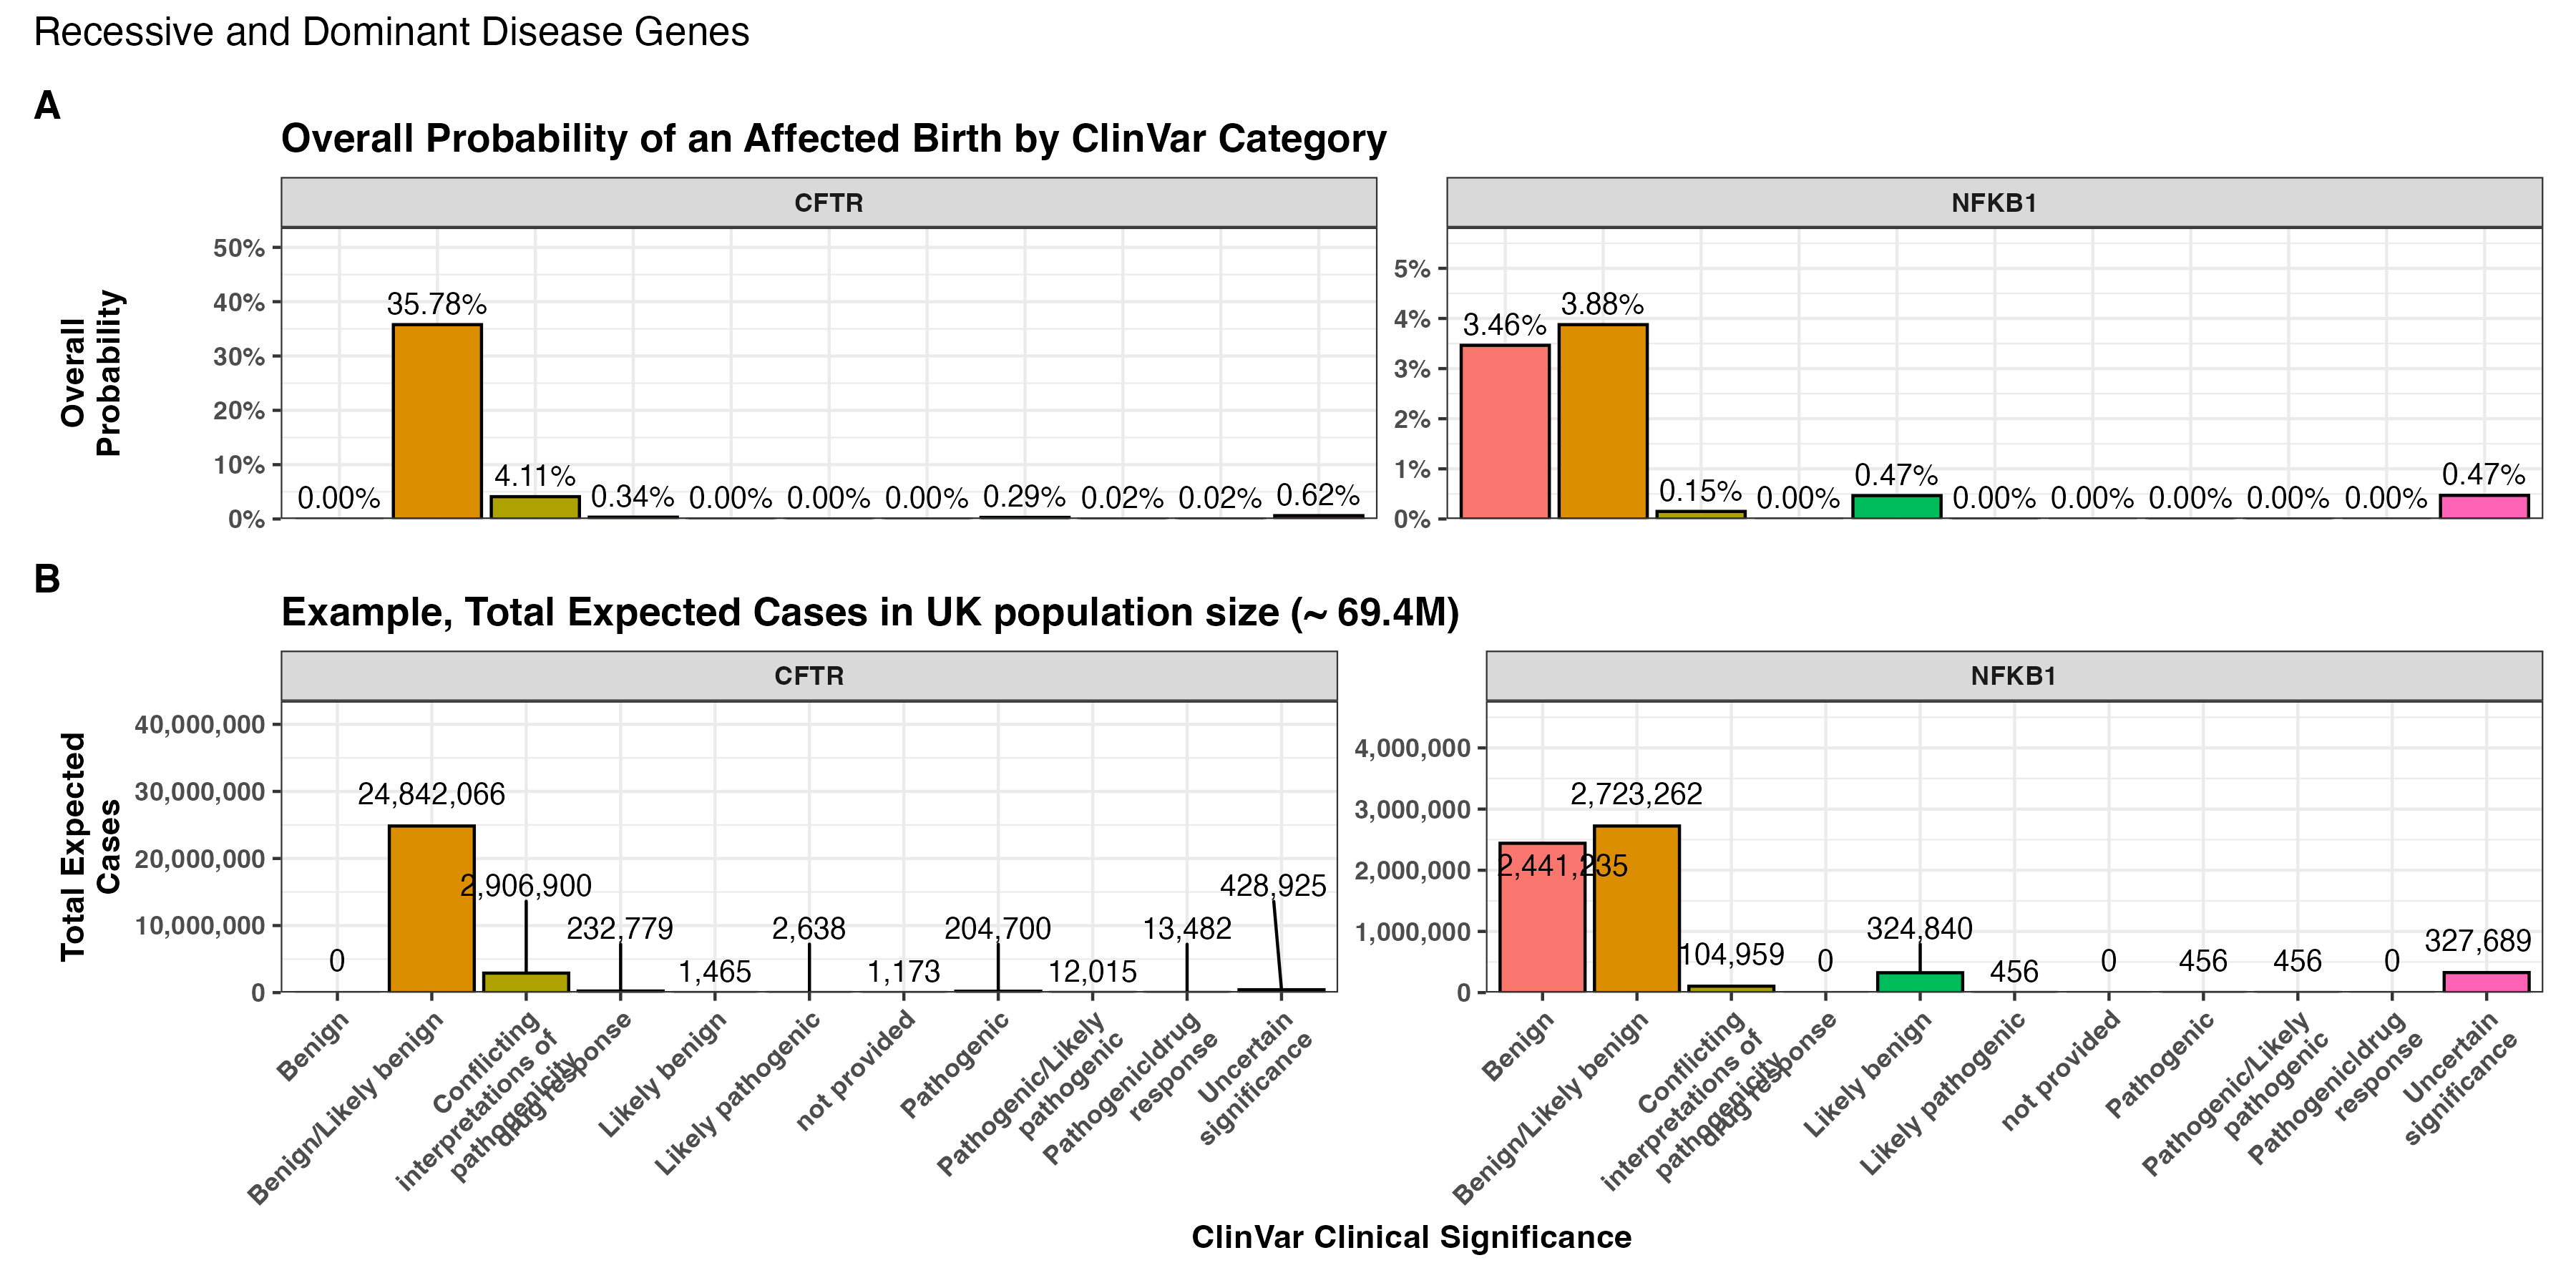
\includegraphics[width=0.99\textwidth]{../images/all_genes_combined_bar_charts_mini.png}
  \caption{\textbf{Combined bar charts summarising the genome-wide analysis of ClinVar clinical significance for the \ac{pid} gene panel}. Panel (A) shows the overall probability of an affected birth by variant classification, and (B) displays the total expected number of cases per classification, both stratified by gene. These integrated results illustrate the variability in variant observations across genes and underpin our validation of the probability estimation framework.}
  \label{fig:all_genes_combined_bar_charts_mini}
\end{figure}

\subsubsection{Validation of SCID-specific disease occurrence}
\begin{figure}[ht]
  \centering
  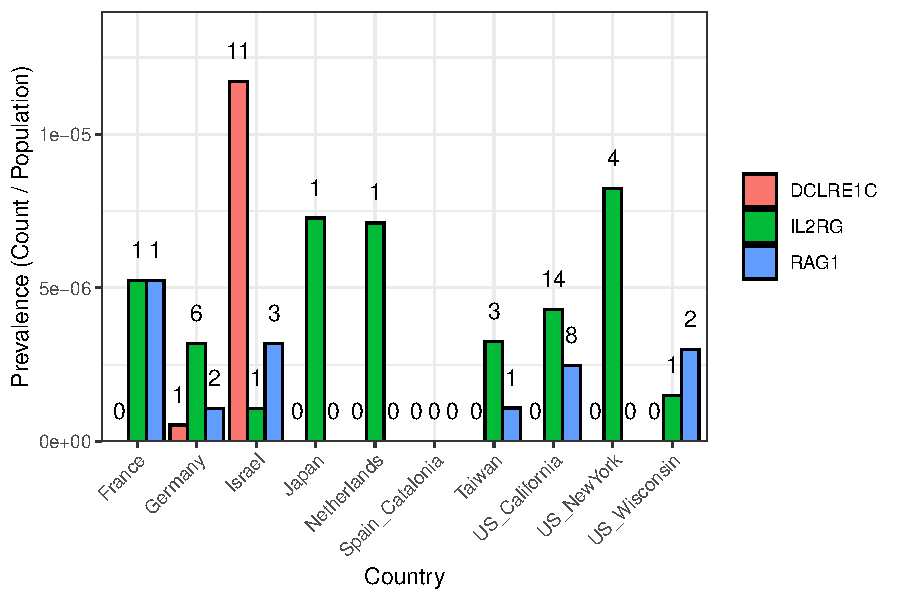
\includegraphics[width=.75\textwidth]{../images/validation_studies_scid_gene_comparison.pdf}
  \caption{\textbf{SCID-specific gene comparison across regions.} The bar plot shows the prevalence of SCID-related cases (count divided by population) for each gene and country (or region), with numbers printed above the bars representing the actual counts in the original cohort (ranging from 0 to 11 per region and gene).}
  \label{fig:scid_gene_comparison}
\end{figure}

\begin{figure}[ht]
  \centering
  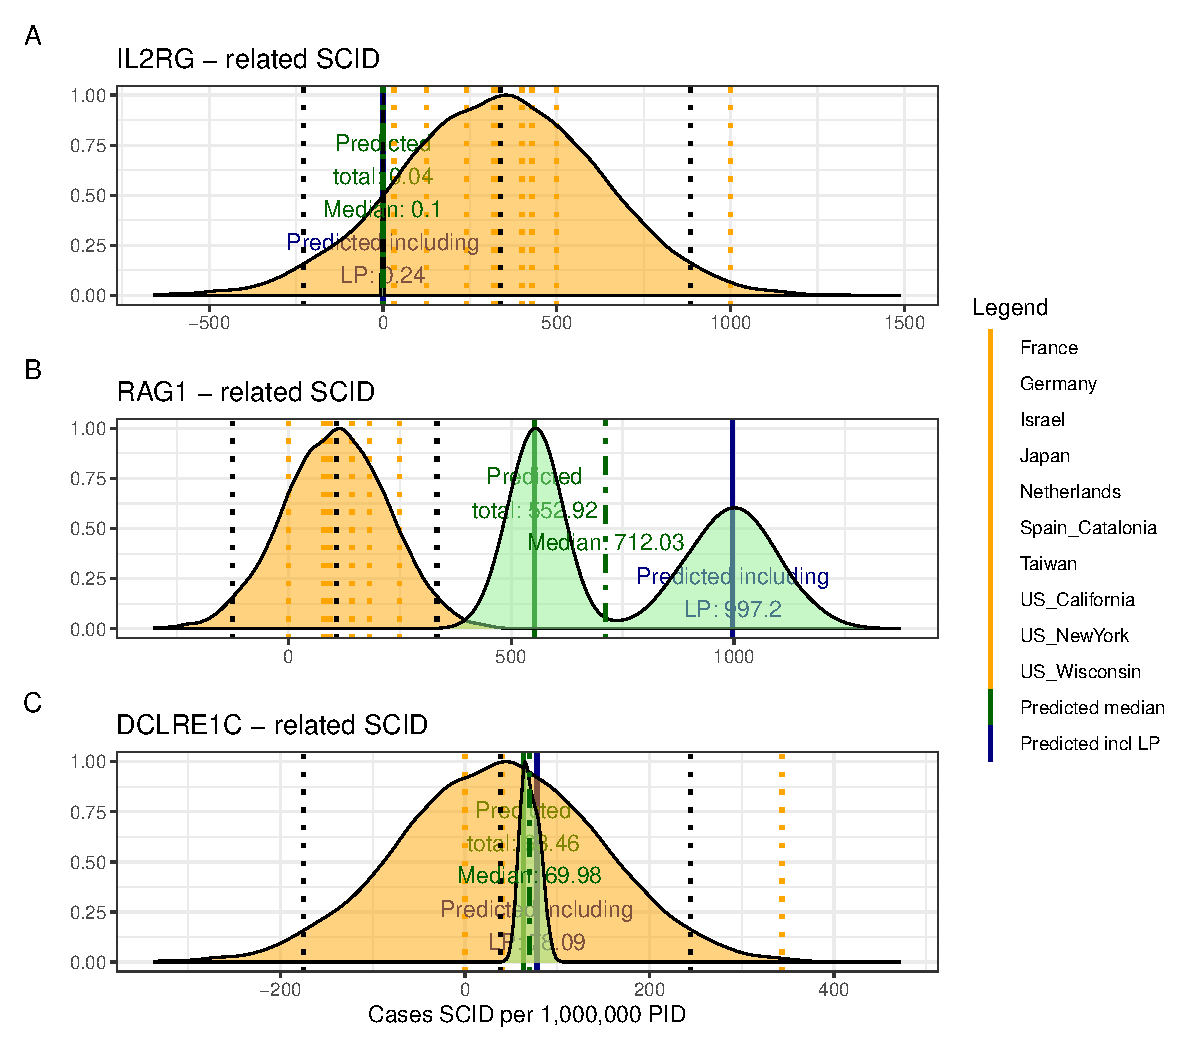
\includegraphics[width=.75\textwidth]{../images/validation_studies_scid_combined_plot.pdf}
  \caption{\textbf{Combined SCID-specific Predictions and Observed Rates per 1,000,000 PID.}
    The figure presents density distributions for the predicted SCID case counts (per 1,000,000 PID) for three genes: \textit{IL2RG}, \textit{RAG1}, and \ac{dclre1c}. Country-specific rates (displayed as dotted vertical lines) are overlaid with the overall predicted distributions for pathogenic and likely pathogenic variants (solid lines with annotated medians). For \textit{IL2RG}, the low predicted value is consistent with the high deleteriousness of loss-of-function variants in this X-linked gene, while \textit{RAG1} exhibits considerably higher predicted counts, reflecting its lower penetrance in an autosomal recessive context.}
  \label{fig:scid_combined}
\end{figure}


\FloatBarrier
\clearpage
\subsection{Genetic constraint in high-impact protein networks}
\subsubsection{Score-positive-total within IEI PPI network}

\begin{figure}[ht]
  \centering
  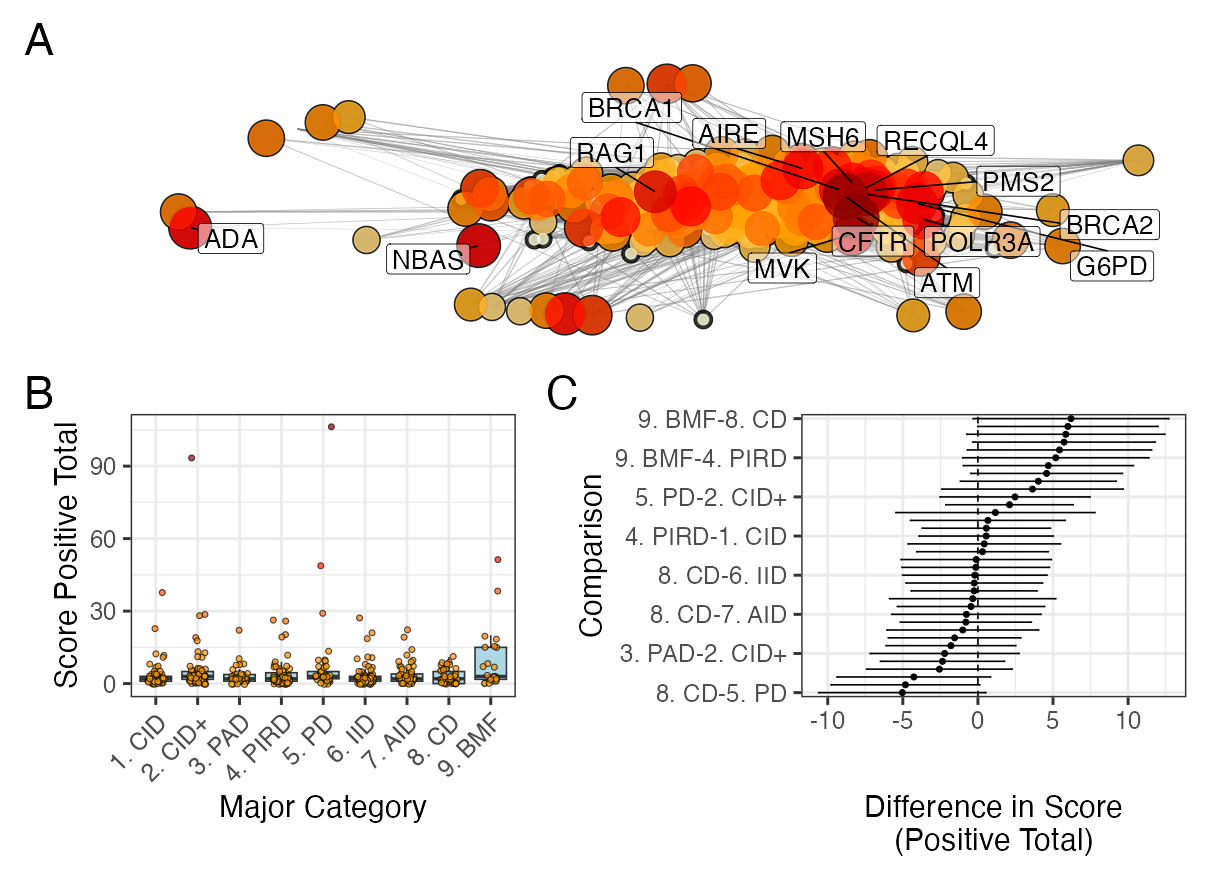
\includegraphics[width=\textwidth]{../images/untangleR_ppi_network_assoc_patch1.jpg}
  \caption{\textbf{\ac{ppi} network and score-positive-total ClinVar significance variants}.
    (A) \ac{ppi} network of disease-associated genes. Node size and colour represent the log-transformed score-positive-total, the top 15 genes/proteins with the highest probability of being observed in disease are labelled.
    (B) Distribution of score-positive-total across the major \ac{iei} disease categories.
    (C) Tukey \ac{hsd} comparisons of mean differences in score-positive-total among all pairwise disease categories. Every 5th label is shown on y-axis.
  }
  \label{fig:ppi_network_assoc}
\end{figure}

\clearpage
\subsubsection{Hierarchical Clustering of Enrichment Scores for Major Disease Categories}

\begin{figure}[ht]
  \centering
  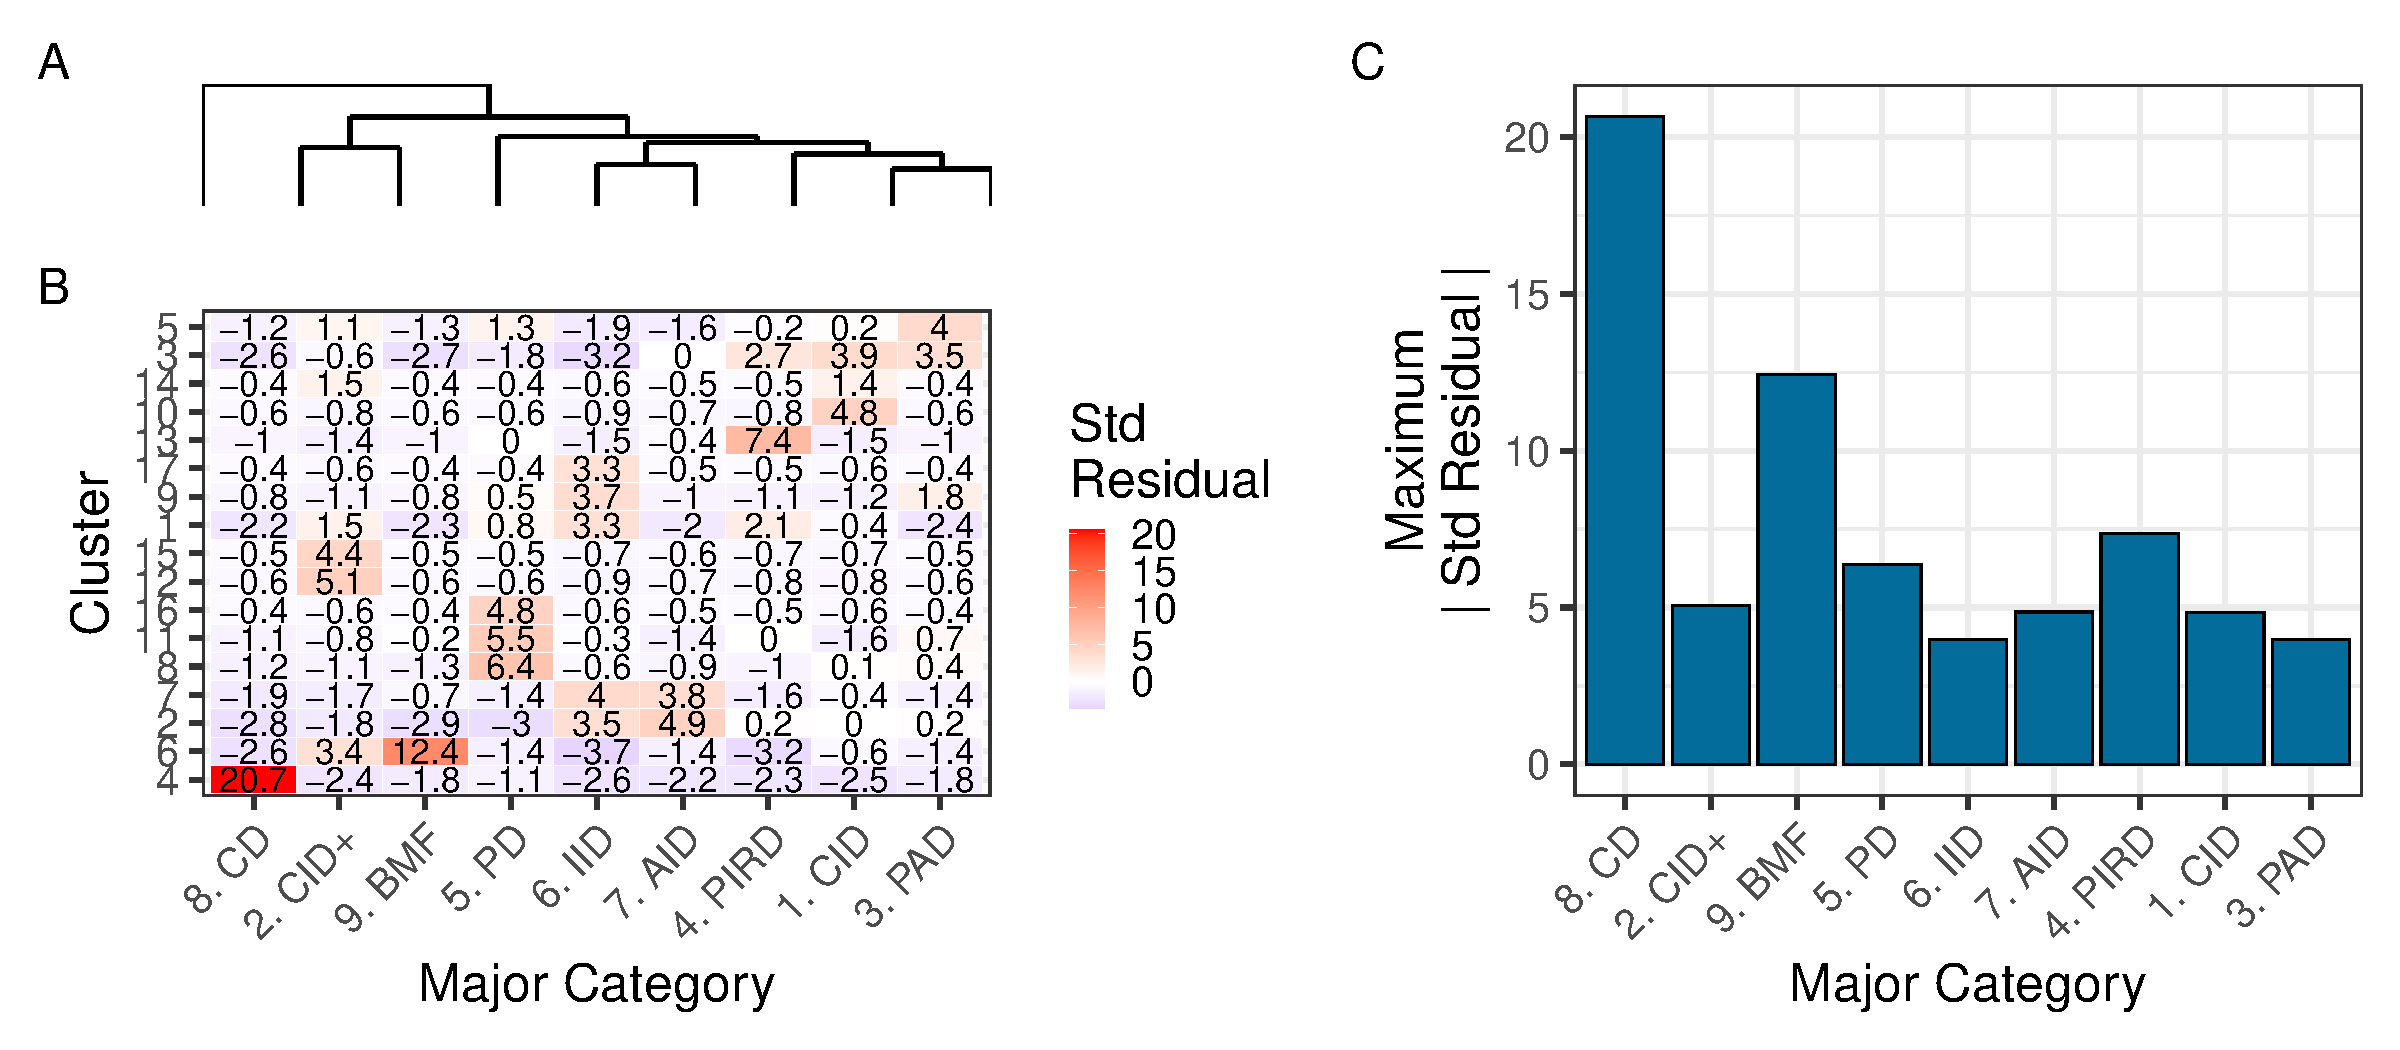
\includegraphics[width=0.99\textwidth]{../images/untangleR_ppi_network_patch2_cator.pdf}
  \caption{
   \textbf{Hierarchical clustering of enrichment scores.}
    The heatmap displays standardised residuals for major disease categories (x-axis) across network clusters (y-axis). A dendrogram groups similar disease categories, and the bar plot shows the maximum absolute residual per category.  (8) \ac{cd} and (9)\ac{bmf} show the highest vales, indicating significant enrichment or depletion (residuals > |2|). Definitions in \textbf{Box \ref{box:definitions}}.
  }
  \label{fig:patch2}
\end{figure}


\FloatBarrier
\clearpage
\subsubsection{PPI connectivity, LOEUF constraint and enriched network cluster analysis}

\begin{figure}[ht]
  \centering
  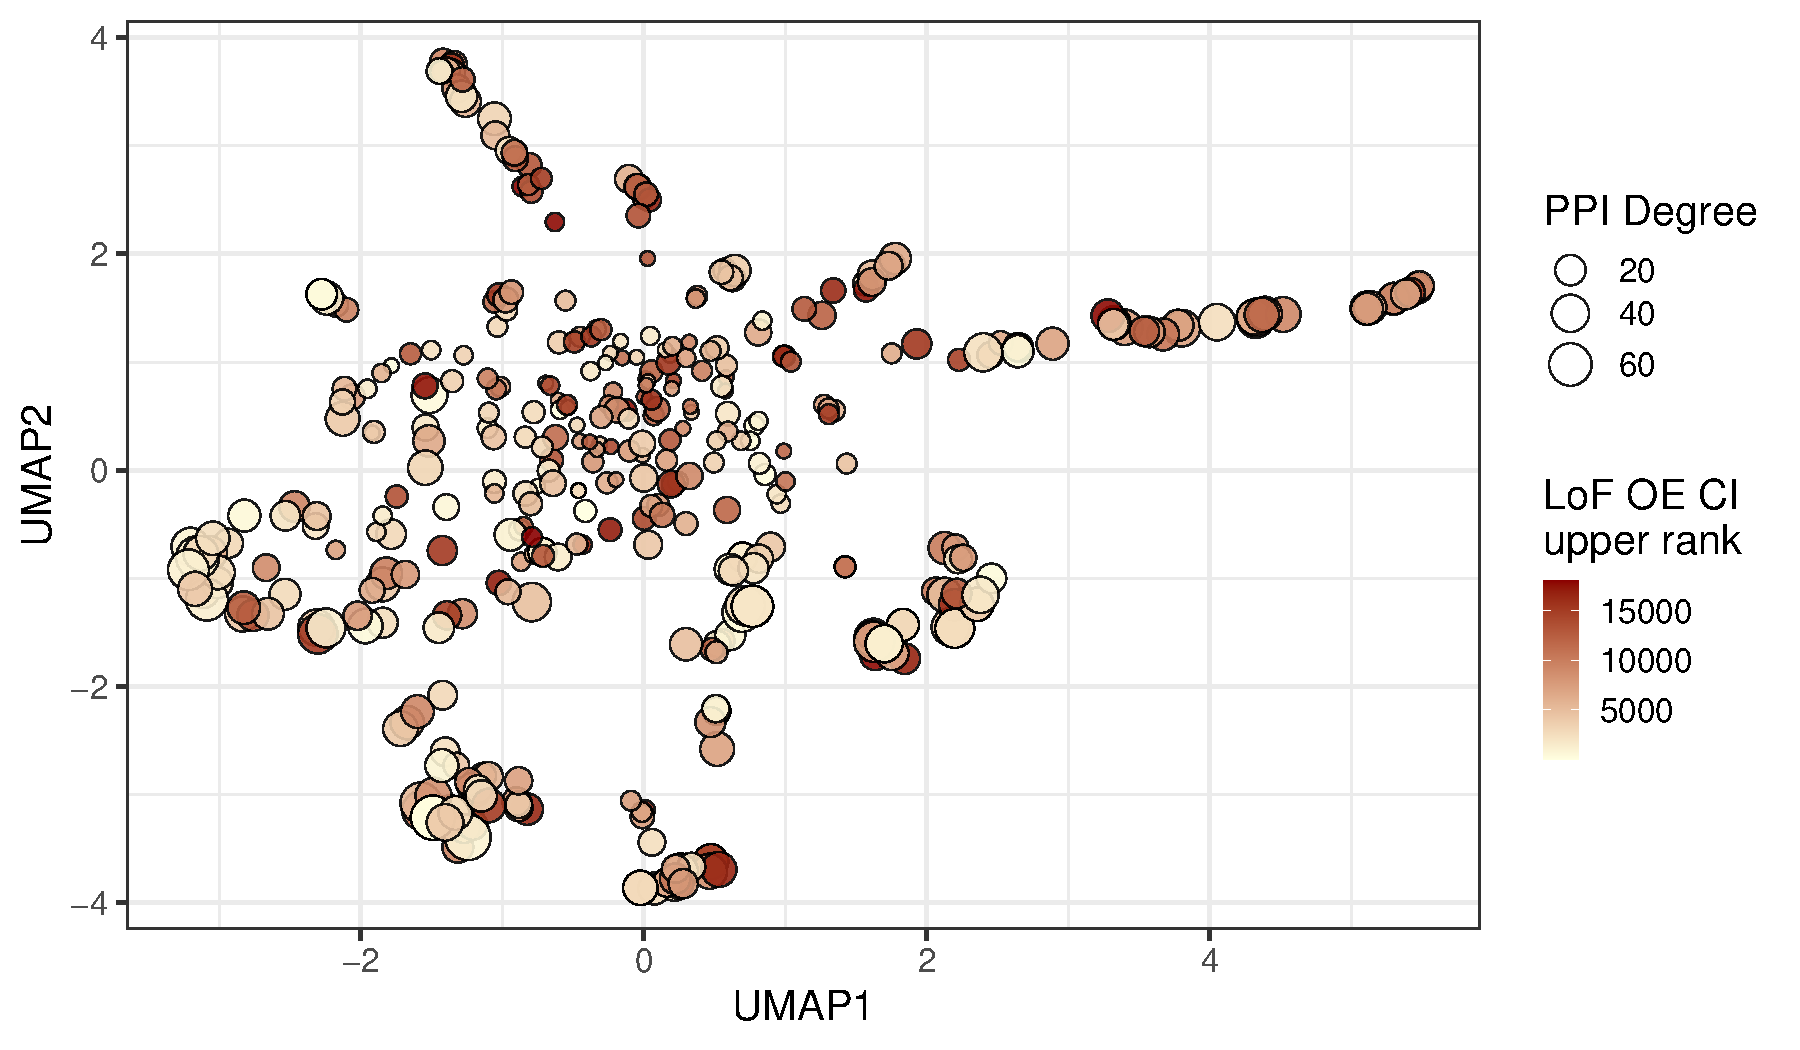
\includegraphics[width=0.99\textwidth]{../images/untangleR_ppi_network_p_umap_const.pdf}
  \caption{
   \textbf{Analysis of \ac{ppi} degree versus \ac{loeuf} upper rank with \ac{umap} embedding of the \ac{ppi} network.}
    The relationship between \ac{ppi} degree (size) and \ac{loeuf} upper rank (color) across gene clusters. No clear patterns are evident.
  }
  \label{fig:p_umap_const}
\end{figure}

\begin{figure}[ht]
  \centering
  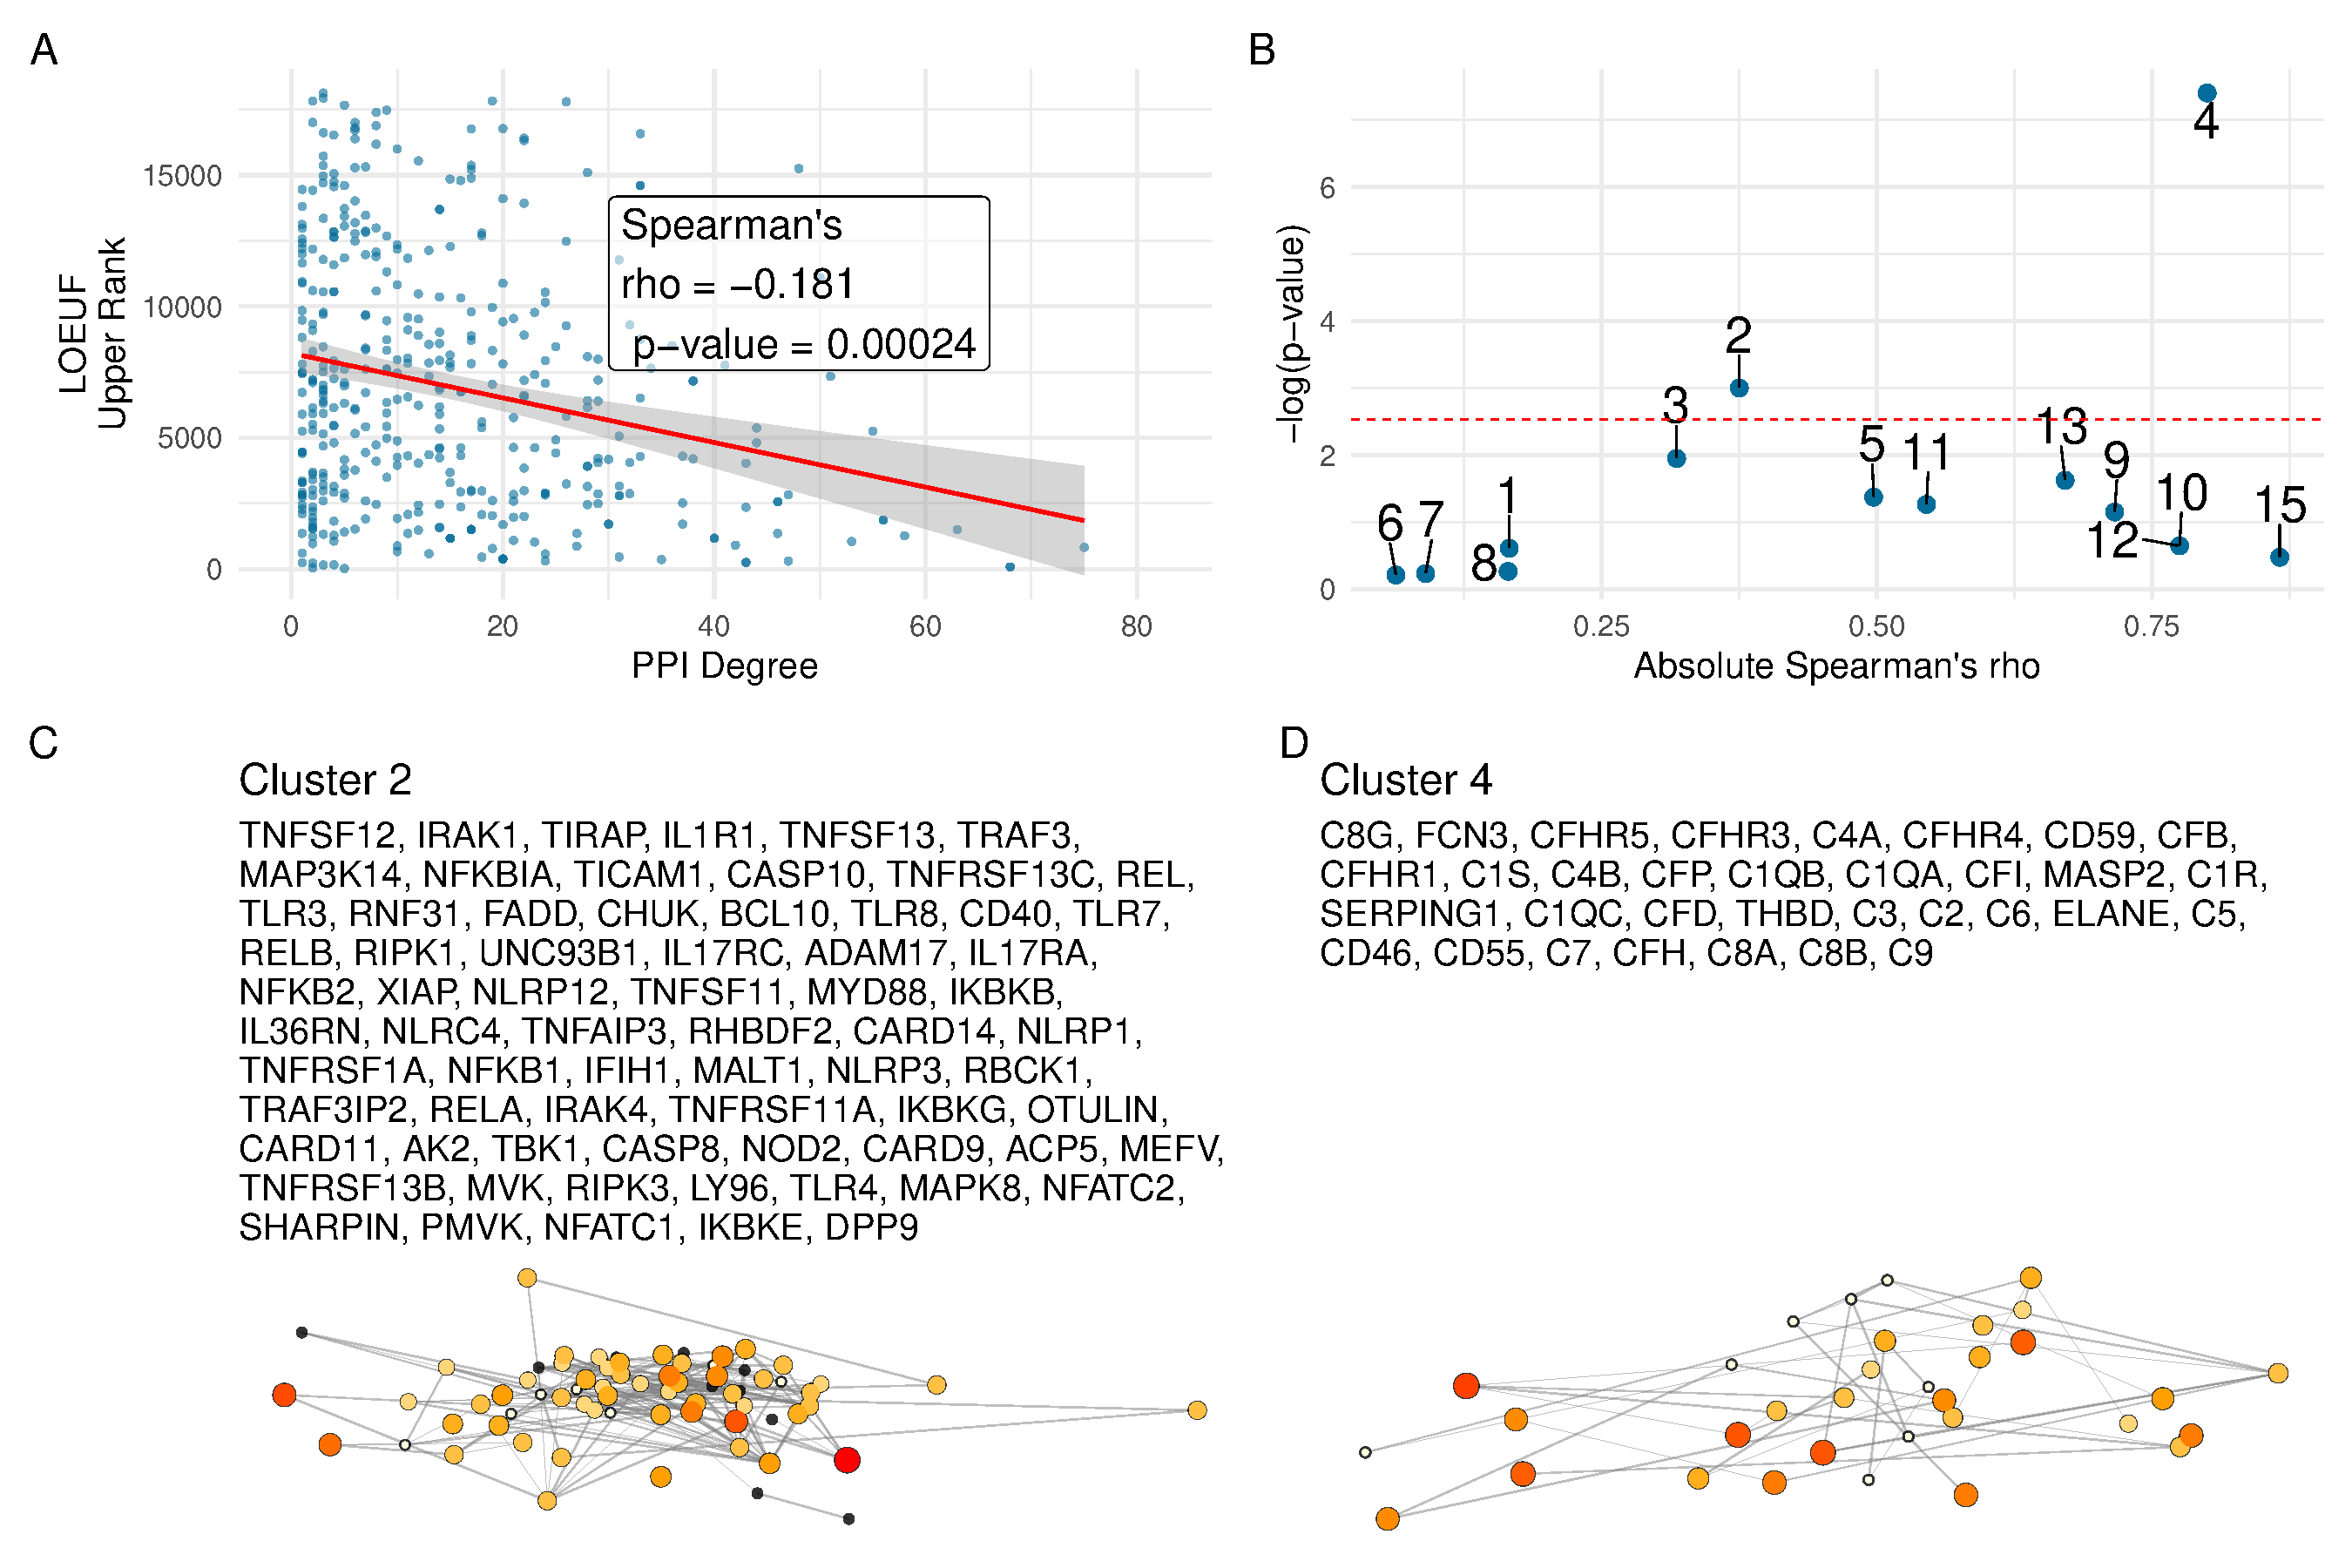
\includegraphics[width=0.99\textwidth]{../images/untangleR_ppi_network_p_cor_spear_rho_sig_clust_patch3.pdf}
  \caption{
    \textbf{Correlation between \ac{ppi} degree and \ac{loeuf} upper rank.} 
    \textbf{(A)} Ananlysis across all genes revealed a weak, significant negative correlation between \ac{ppi} degree and \ac{loeuf} upper rank. \textbf{(B)} The cluster-wise analysis showed that clusters 2 and 4 exhibited moderate to strong correlations, while other clusters display weak or non-significant relationships. \textbf{(C) and (D)} Shows the new network plots for the significantly enriched clusters based on \ac{gnomad} constraint metrics.
  }
  \label{fig:p_cor_spear_rho_sig_clust_patch3}
\end{figure}

\begin{figure}[ht]
\centering
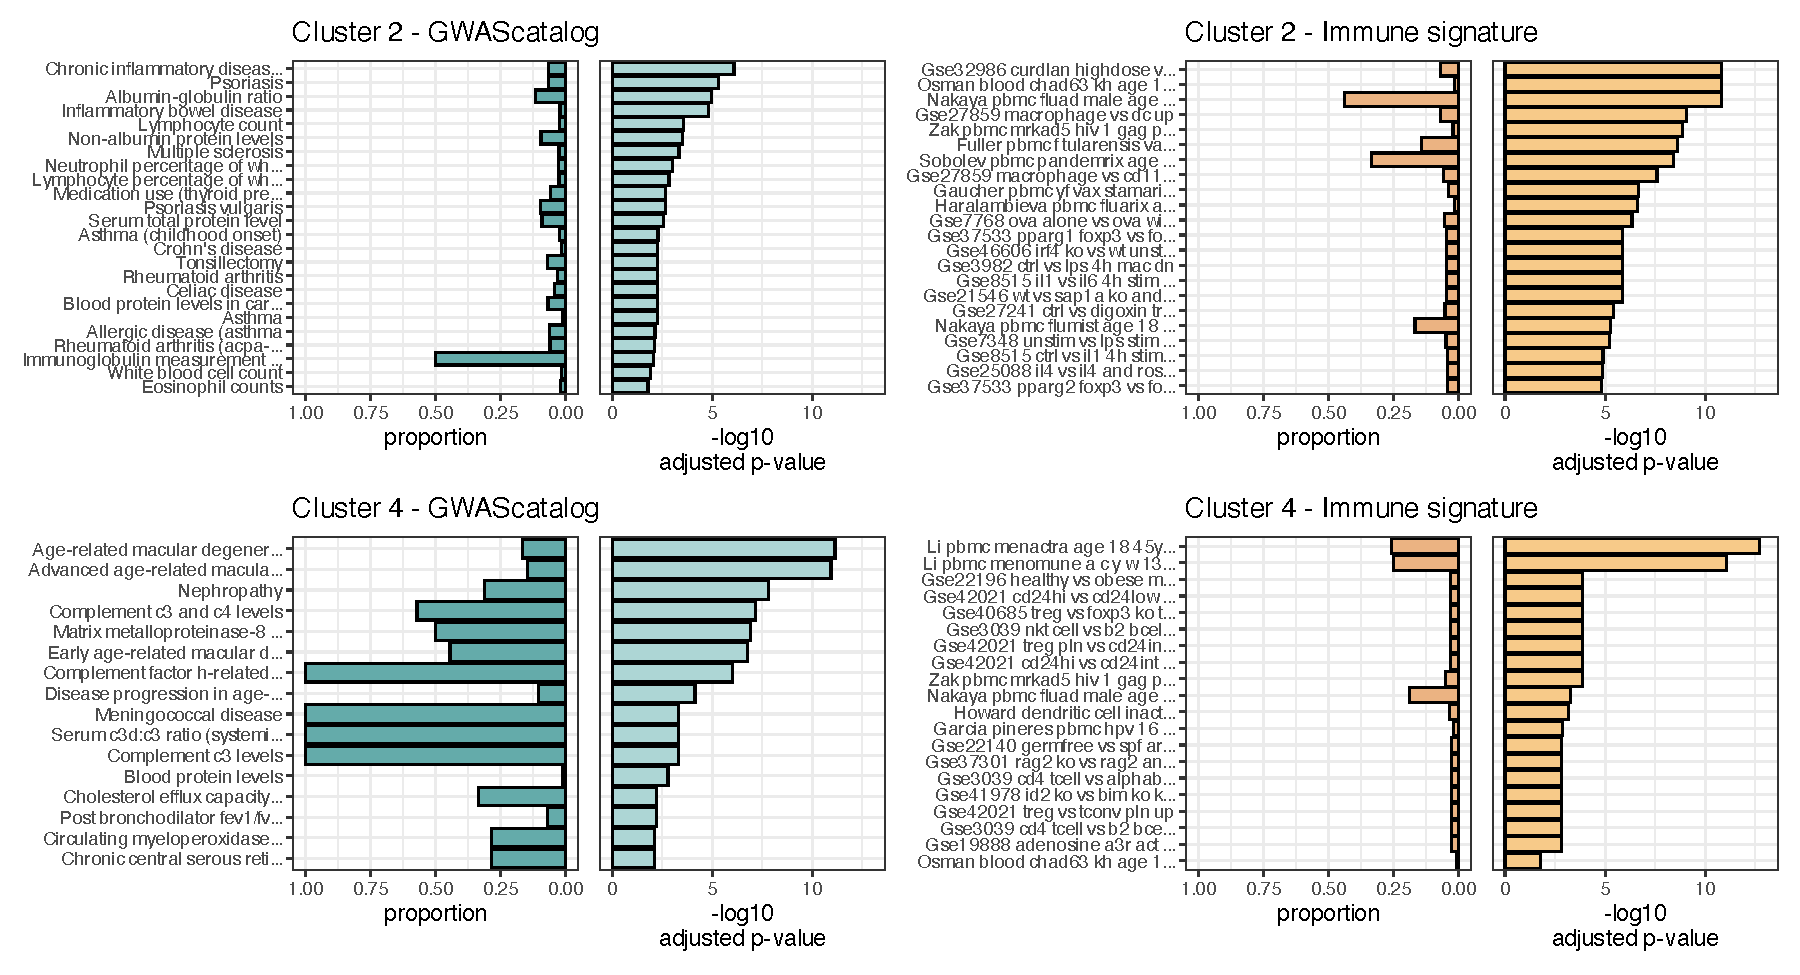
\includegraphics[width=0.99\textwidth]{../images/fuma_merge.pdf}
\caption{\textbf{Composite Enrichment Profiles for \ac{iei} Gene Sets.} 
We selected the top two enriched clusters (as per \textbf{Figure \ref{fig:p_cor_spear_rho_sig_clust_patch3}}) and performed functional enrichment analysis derived from known disease associations. For each gene set, the left panel displays the proportion of input genes overlapping with a curated gene set, and the right panel shows the \(-\log_{10}\) adjusted p-value from hypergeometric testing. These profiles, stratified by cluster (Cluster 2 and Cluster 4) and by gene set category (GWAScatalog and Immunologic Signatures), highlight distinct enrichment patterns that reflect differential pathogenic variant loads in the \ac{iei} gene panels.}
\label{fig:fuma_merge}
\end{figure}

\begin{figure}[ht]
\centering
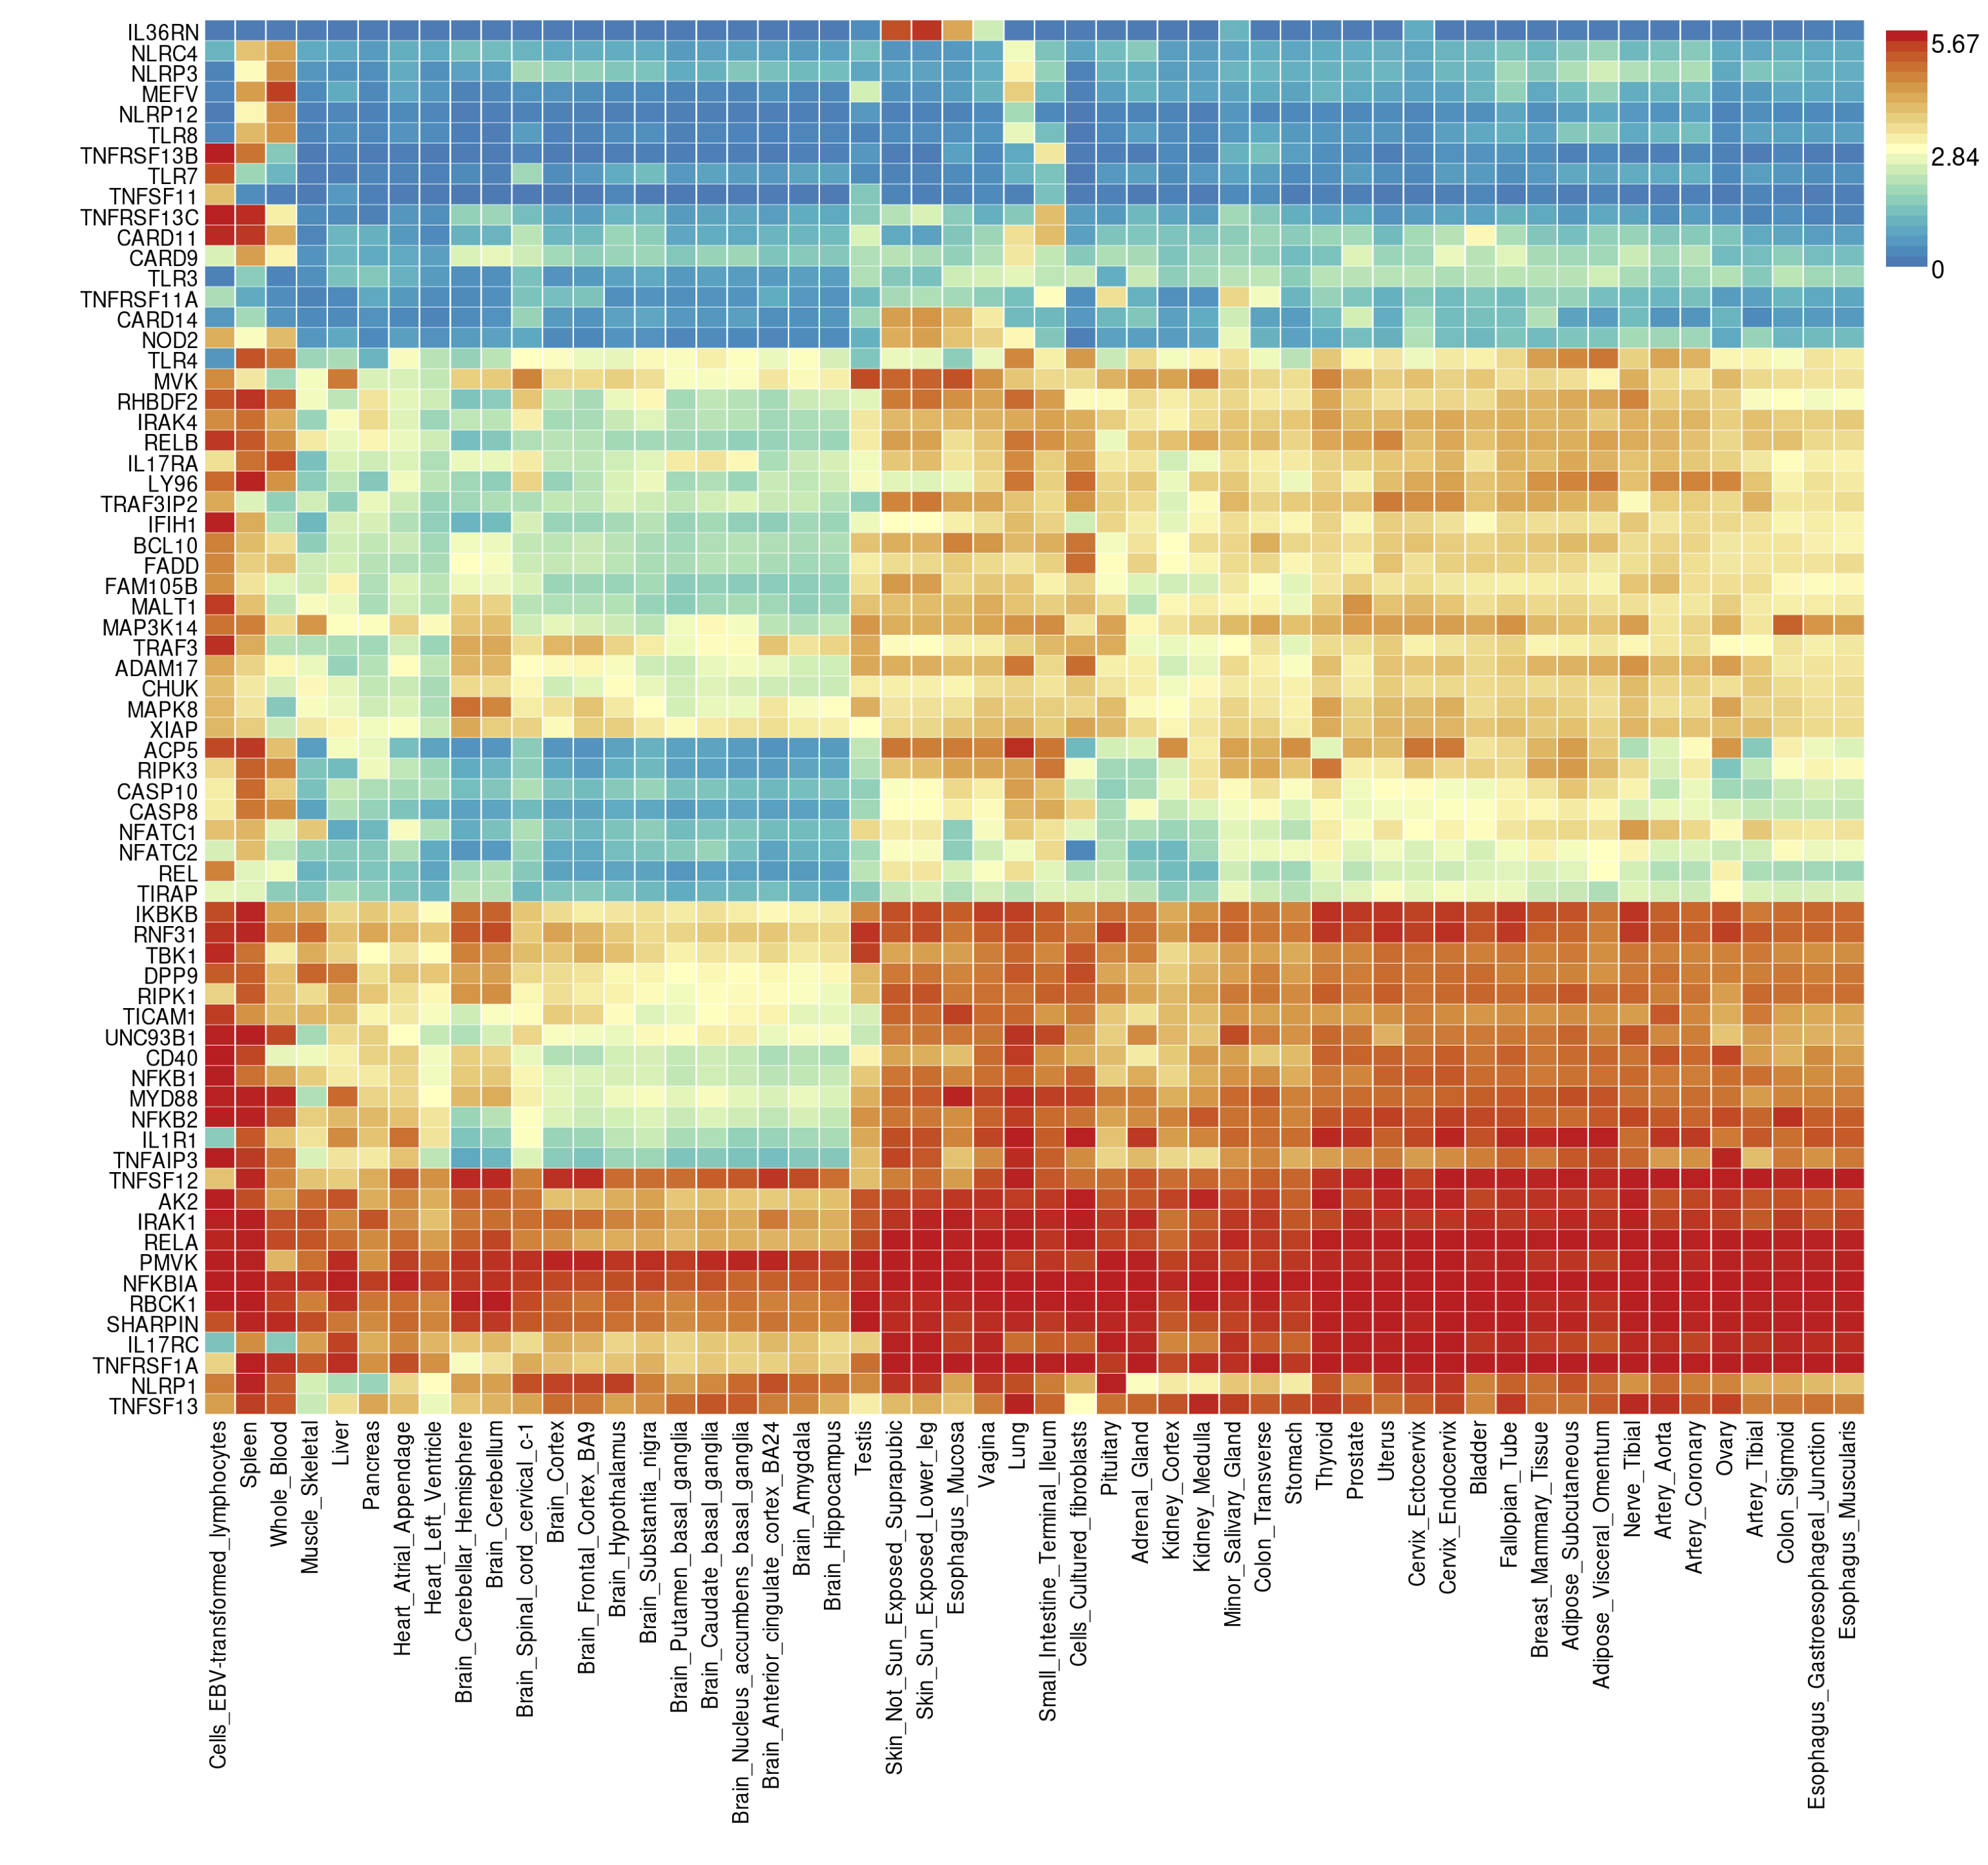
\includegraphics[width=0.75\textwidth]{../images/expHeat_FUMA_jobs604419_var_risk_est_cluster_2.png}
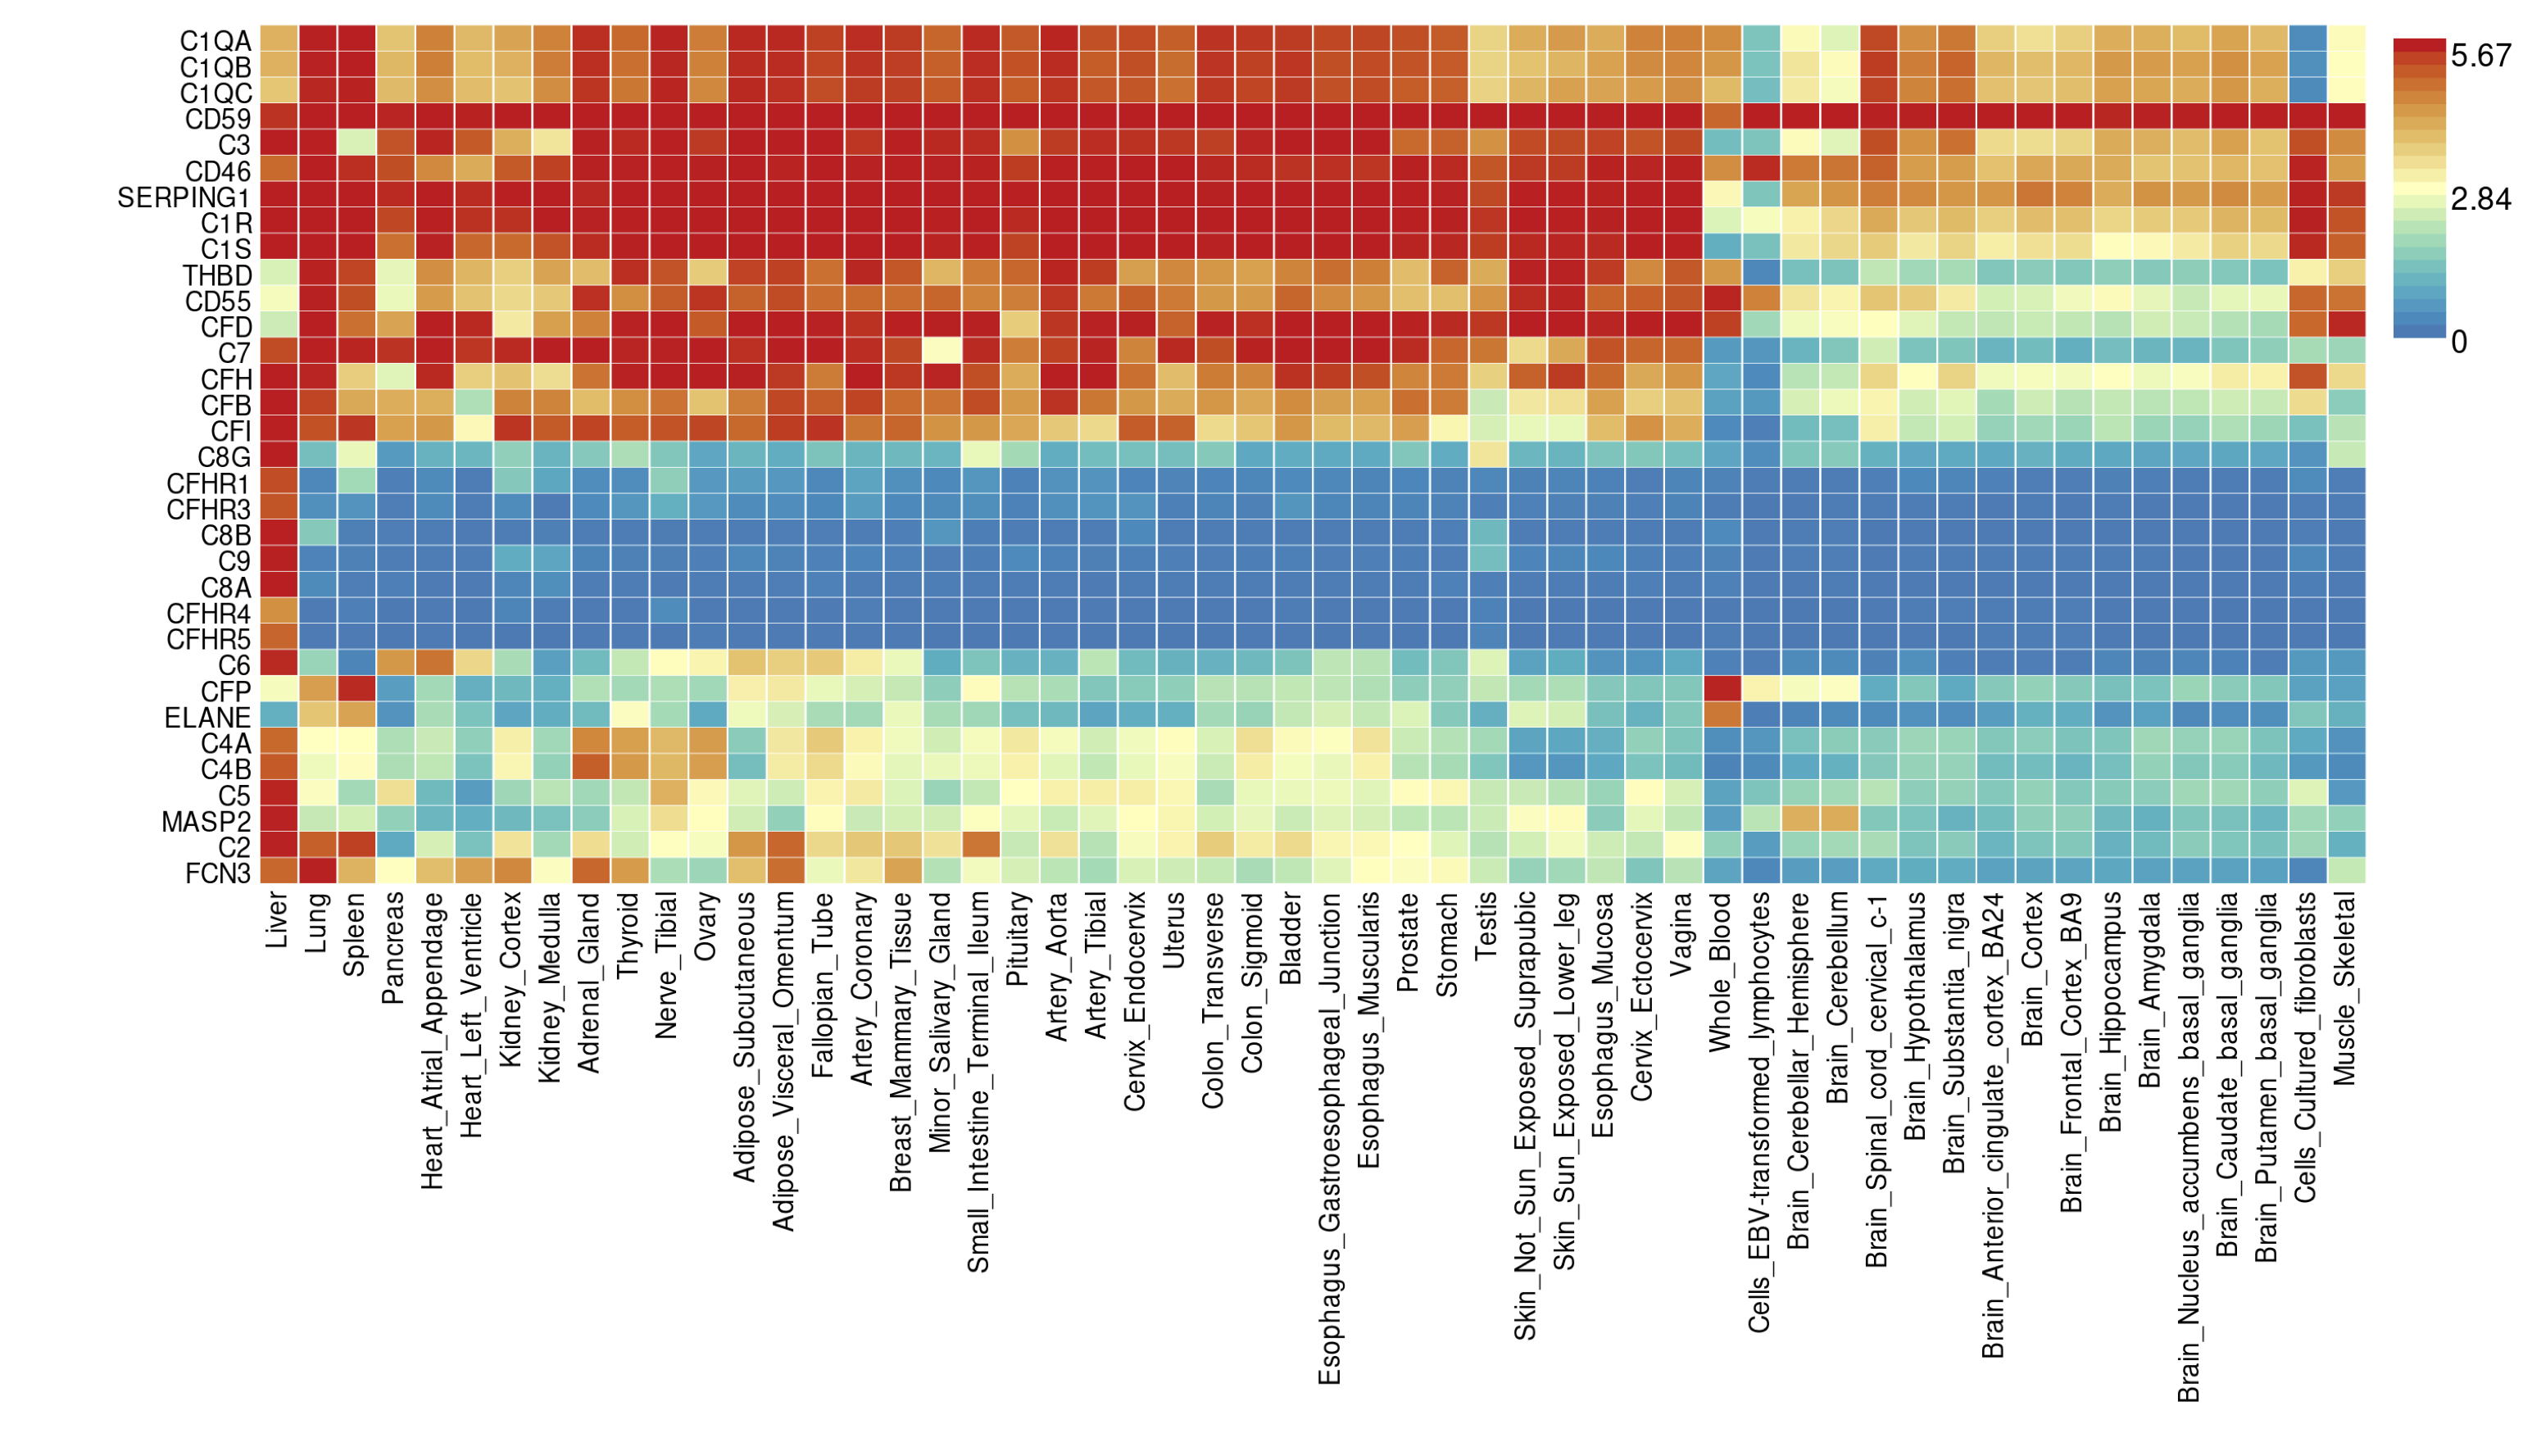
\includegraphics[width=0.75\textwidth]{../images/expHeat_FUMA_jobs604403_var_risk_est_cluster_4.png}
\caption{\textbf{Gene Expression Heatmaps for IEI Genes.} GTEx v8 data from 54 tissue types display the average expression per tissue label (log\(_2\) transformed) for the IEI gene panels. Top: Cluster 2; Bottom: Cluster 4.}
\label{fig:expHeatmaps}
\end{figure}





\FloatBarrier
\clearpage
\subsection{Novel PID classifications derived from genetic PPI and clinical features}

\begin{figure}[ht]
  \centering
  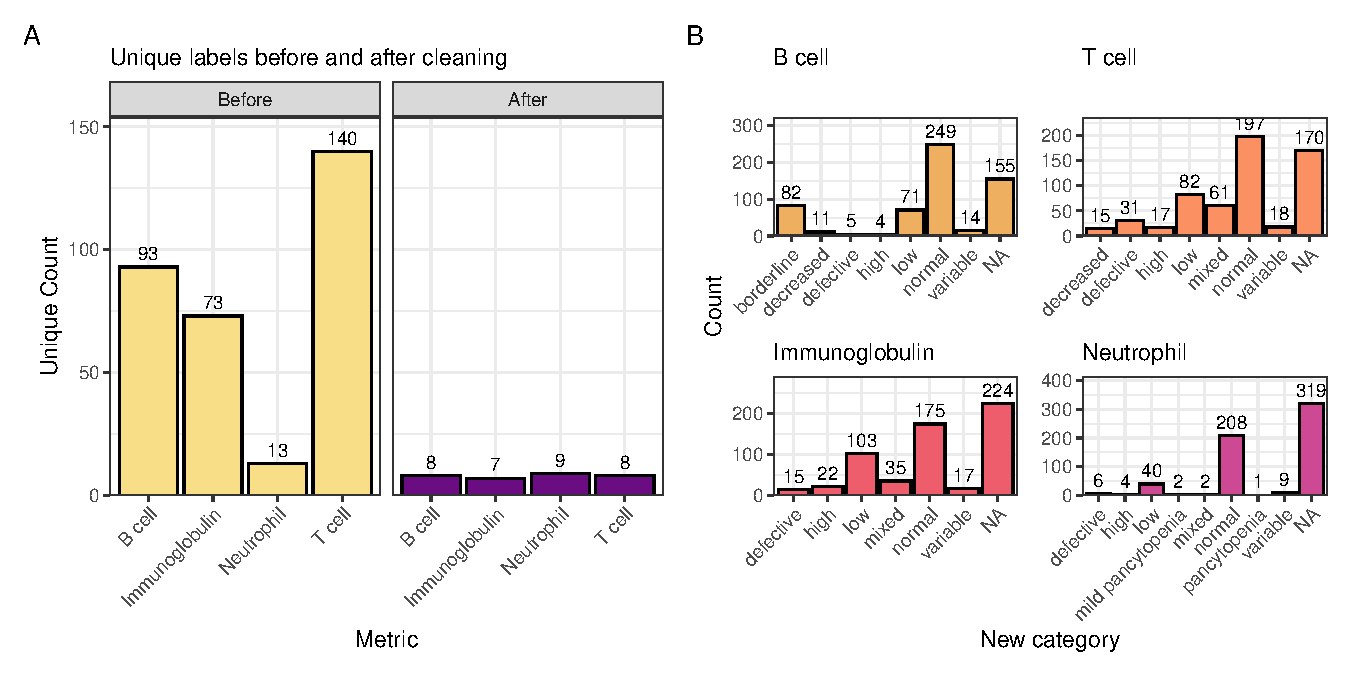
\includegraphics[width=0.99\textwidth]{../images/plot_patch1.pdf}
 %   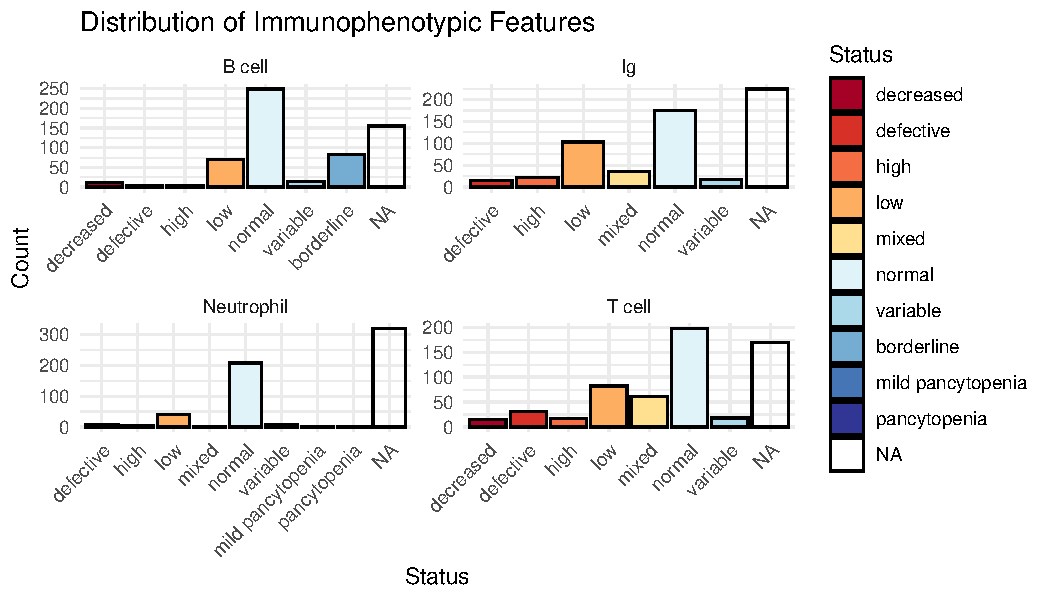
\includegraphics[width=0.7\textwidth]{../images/plot_patch_1_v2.pdf}
  \caption{ \textbf{Distribution of immunophenotypic features before and after recategorisation.}
  The original \ac{iuis} \ac{iei} descriptions contain information such as T cell-related
  ``decreased CD8, normal or decreased CD4 cells'' which we recategorise as ``low''.
  The bar plot shows the count of unique labels for each status (normal, not\_normal) across the T cell, B cell, \ac{ig}, and Neutrophil features.}
  \label{fig:immunophenotype_before_after}
\end{figure}


\begin{figure}[ht]
  \centering
  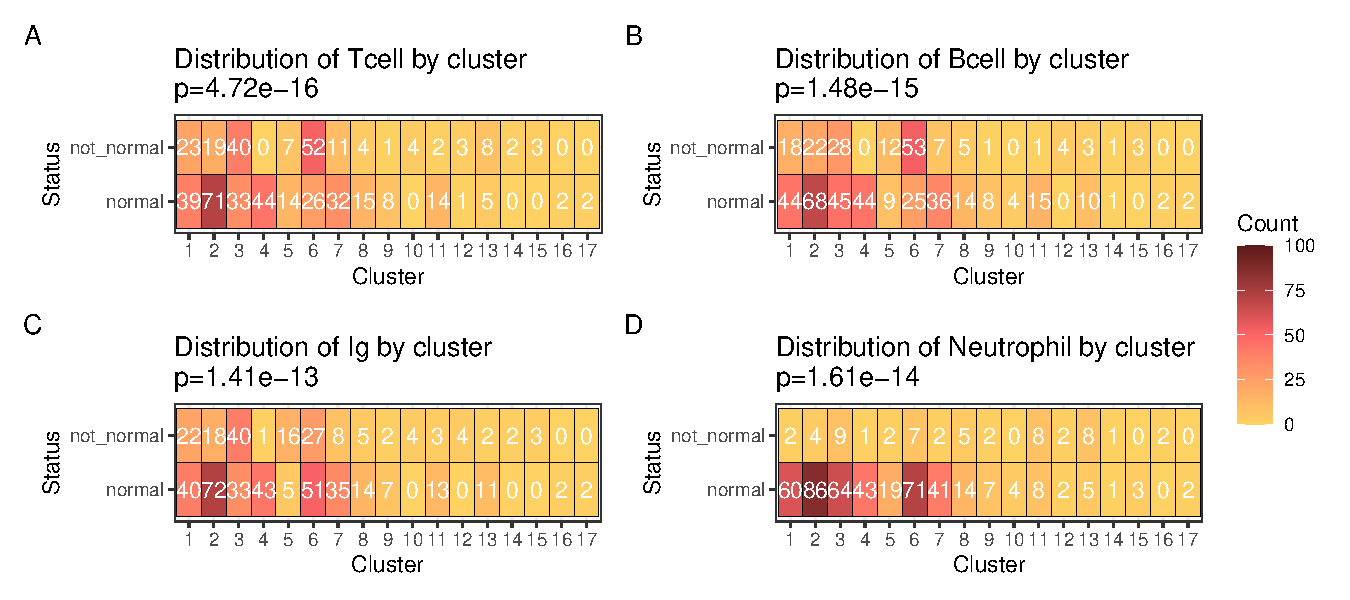
\includegraphics[width=0.99\textwidth]{../images/plot_multicat_patch_3_clust_chi.pdf}
  \caption{\textbf{Heatmaps of clinical feature distributions by \ac{ppi} cluster.} The heatmaps display the count of observations for abnormality of each clinical feature (A) T cell, (B) B cell, (C) Immunoglobulin, (D) Neutrophil, in relation to the \ac{ppi} clusters, with p-values from chi-square tests annotated in the titles.}
  \label{fig:plot_multicat_patch_3_clust_chi}
\end{figure}

\begin{figure}[ht]
  \centering
  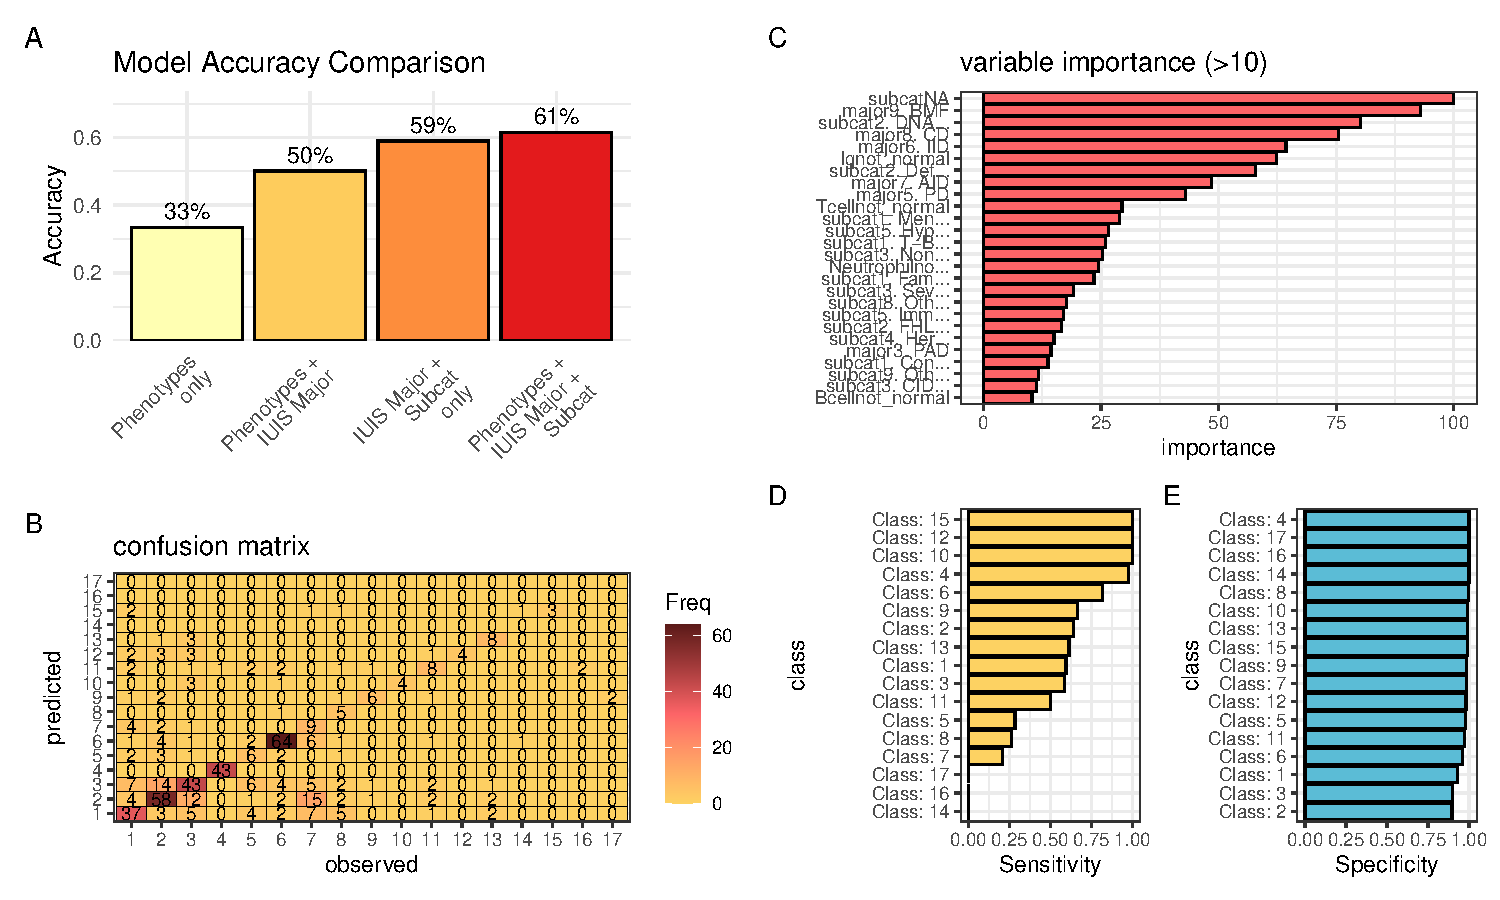
\includegraphics[width=0.99\textwidth]{../images/plot_multicat_performance_combined.pdf}
  \caption{\textbf{Performance comparison of PID classifiers.} Classification predicting \ac{ppi} cluster membership from \ac{iuis} major category, subcategory, and immunological features. (A) Overall accuracy for four rpart models
used to predict \ac{ppi} clustering. The combined model achieves 61.4 \% accuracy, exceeding all simpler approaches. 
Nodes were split to minimize Gini impurity, pruned by cost-complexity (cp = 0.001), and validated via 5‑fold cross‑validation. %Terminal leaves display the assigned cluster and the proportion of genes falling into each group. 
(B-E) The summary statistics from the top model are detailed.  
}
  \label{fig:multicat_performance_combined}
\end{figure}

%\begin{figure}[ht]
%  \centering
%  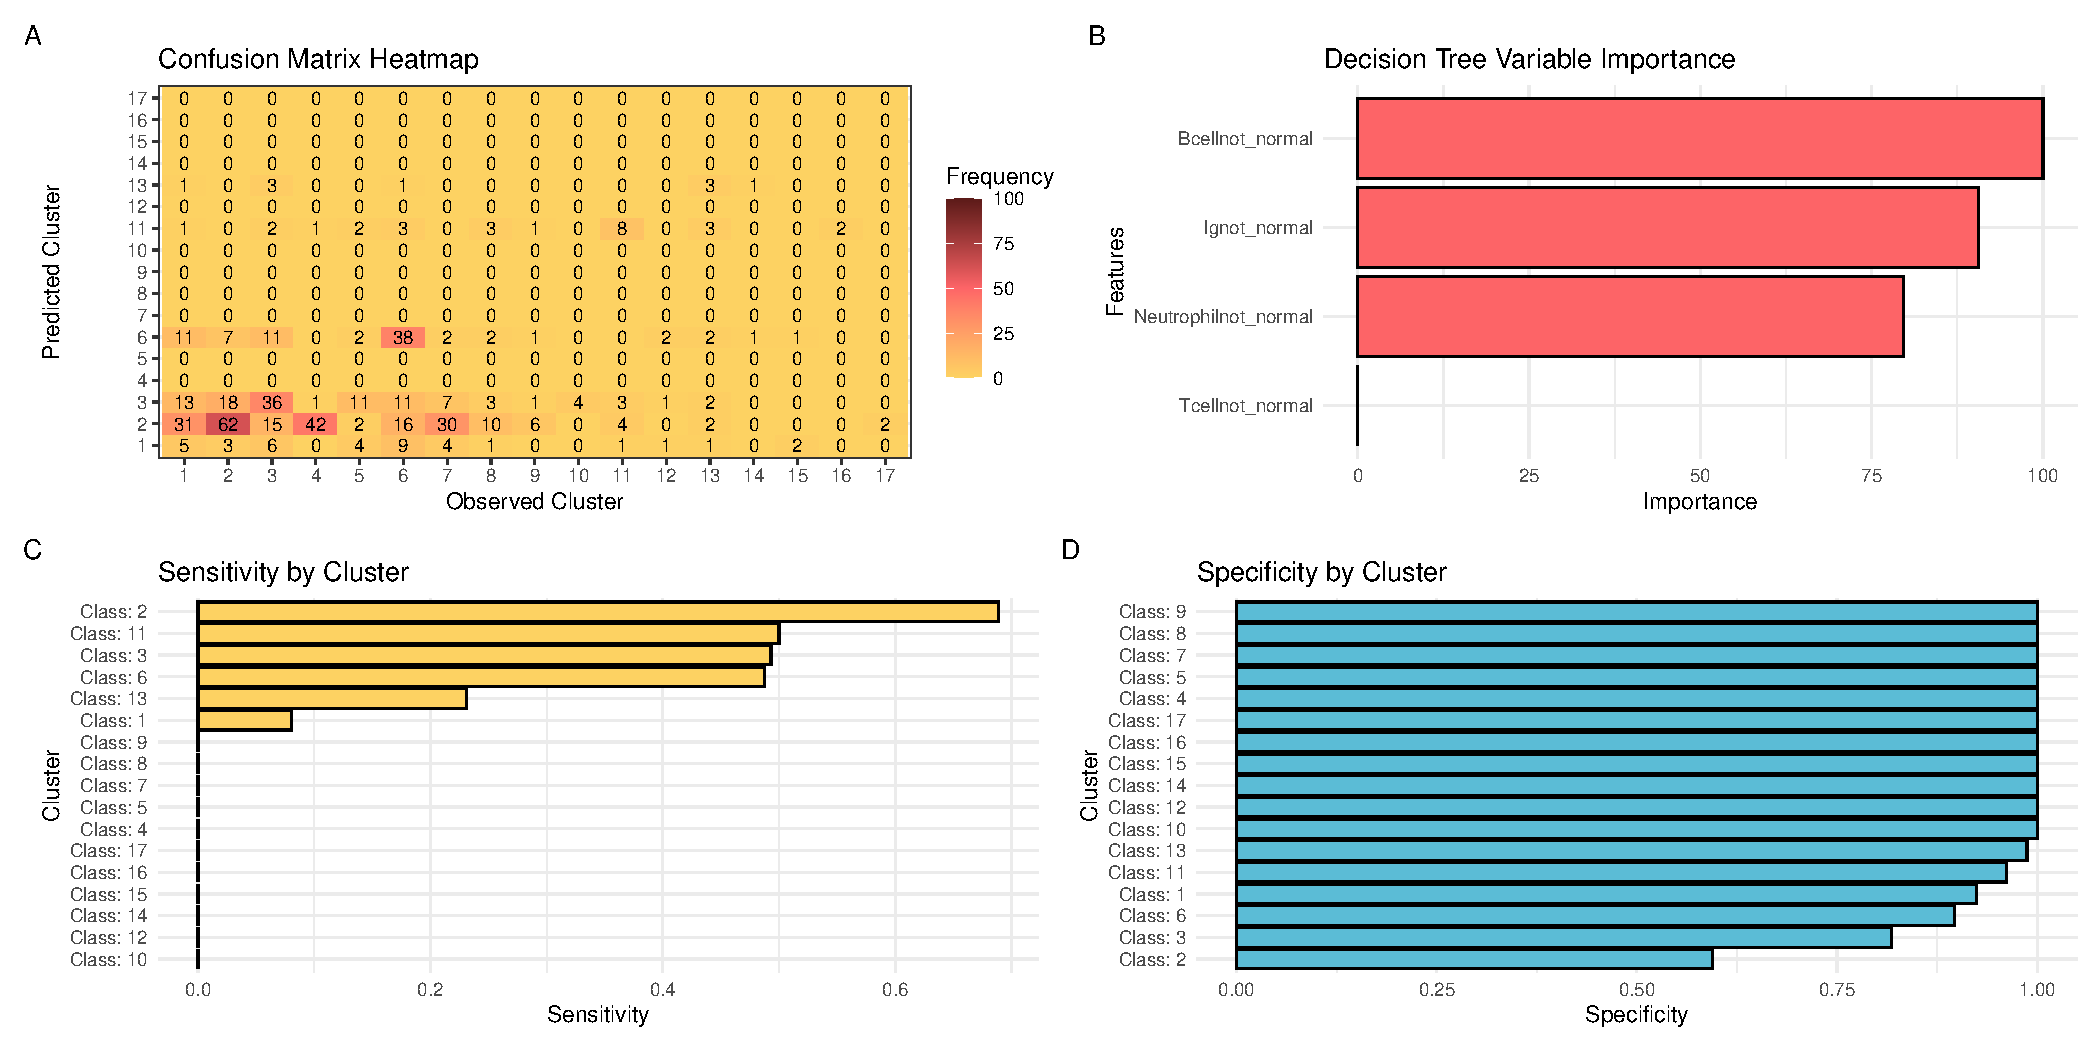
\includegraphics[width=0.99\textwidth]{../images/plot_combined_model_interpret_fine.pdf}
%  \caption{\textbf{Model performance for fine-tuned \ac{pid} classification.} (A) Confusion matrix heatmap comparing observed and predicted \ac{ppi} clusters. (B) Variable importance plot ranking immunophenotypic features contributing to the classifier. (C) Per-class sensitivity and (D) per-class specificity bar plots. These panels collectively demonstrate the performance of the decision tree classifier in stratifying \ac{pid} genes based on immunophenotypic and \ac{ppi} features.}
%  \label{fig:confusion_matrix}
%\end{figure}

\FloatBarrier
\clearpage
\subsection{Probability of observing AlphaMissense pathogenicity}

\begin{figure}[ht]
  \centering
  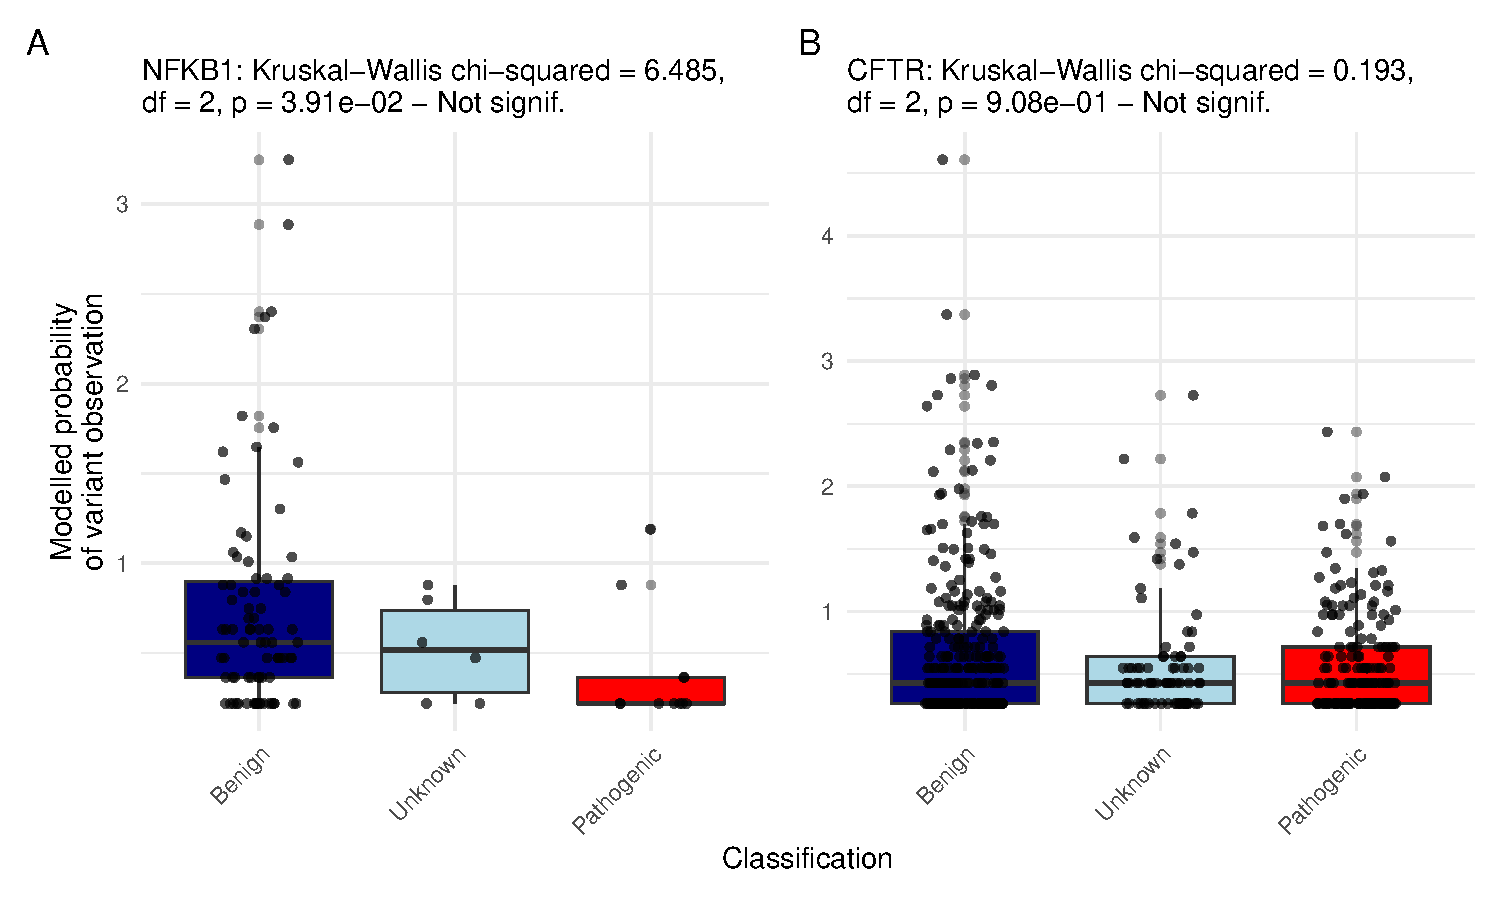
\includegraphics[width=0.99\textwidth]{../images/p_alphamissense_kw.pdf}
  \caption{\textbf{Observed Disease Probability by Clinical Classification with AlphaMissense.} The figure displays the Kruskal-Wallis test results for NFKB1 and CFTR, showing no significant differences.}
  \label{fig:alphamissense_kw}
\end{figure}

\FloatBarrier
\end{document}




